\documentclass[10pt,openany]{article}
\usepackage{ctex} 
\usepackage{geometry,graphicx,xcolor,color}
\geometry{
	a4paper,
	top=25.4mm, bottom=25.4mm,
	left=20mm, right=20mm,
	headheight=2.17cm,
	headsep=4mm,
	footskip=12mm
}
\usepackage[all,pdf]{xy}
\usepackage{amssymb,amsmath,mathrsfs}             
\usepackage{mathpazo}
\usepackage[nofontspec]{newpxtext}
\usepackage{array}
\usepackage{amsmath}
\usepackage{amssymb}
\usepackage{enumerate}
\usepackage{amsthm}
\usepackage{bm}
\usepackage{mathtools}
\usepackage{mathrsfs}
\usepackage{tcolorbox}
\usepackage{indentfirst}
\usepackage{setspace}
\usepackage{subfigure} 
\usepackage{tkz-fct}
\usetikzlibrary{calc,intersections,through,backgrounds,3d}
\usepackage{tkz-euclide}
\usepackage{tikz-3dplot}
\usepackage{pgfplots}
\usepackage{booktabs}
\usepackage{float}
\usepackage[graphicx]{realboxes}
\usepackage{fancyhdr}
\usepackage{nicematrix}
\definecolor{winered}{rgb}{0.5,0,0}
\definecolor{structurecolor}{RGB}{122,122,142}
\definecolor{main}{HTML}{3D445F}
\definecolor{second}{HTML}{627581}
\definecolor{third}{HTML}{333333}
\definecolor{deepgreen}{HTML}{2F5E4E}  
\definecolor{purple}{HTML}{512E5F}   

\usepackage{hyperref}
\hypersetup{colorlinks = true, linktoc=all, linkcolor=blue, urlcolor=winered}


\usepackage{amsthm}
% 设定颜色(假设你在别处定义了 \color{main} 等)
\usepackage{xcolor}
\usepackage{etoolbox}
% 定义定理风格
\usepackage{amsthm}
\newtheoremstyle{defstyle}
{0.3cm}{0.3cm}{\fangsong}{-1cm}{\bfseries\color{main}}{}{0.5em}
{\indent 【\thmname{#1} \thmnumber{#2}】\ifthenelse{\equal{#3}{}}{}{~\thmnote{(#3)}}}

\newtheoremstyle{thmstyle}
{0.3cm}{0.3cm}{\kaishu}{-1cm}{\bfseries\color{second}}{}{0.5em}
{\indent 【\thmname{#1} \thmnumber{#2}】\ifthenelse{\equal{#3}{}}{}{~\thmnote{(#3)}}}

\newtheoremstyle{remstyle}
{0.3cm}{0.3cm}{\kaishu}{-1cm}{\bfseries\color{third}}{}{0.5em}
{\indent 【\thmname{#1} \thmnumber{#2}】\ifthenelse{\equal{#3}{}}{}{~\thmnote{(#3)}}}

\newtheoremstyle{exastyle}
{0.3cm}{0.3cm}{\kaishu}{-1cm}{\bfseries\color{deepgreen}}{}{0.5em}
{\indent 【\thmname{#1} \thmnumber{#2}】\ifthenelse{\equal{#3}{}}{}{~\thmnote{(#3)}}}

\newtheoremstyle{prostyle}
{0.3cm}{0.3cm}{\kaishu}{-1cm}{\bfseries\color{purple}}{}{0.5em}
{\indent 【\thmname{#1} \thmnumber{#2}】\ifthenelse{\equal{#3}{}}{}{~\thmnote{(#3)}}}

\theoremstyle{thmstyle} %theorem style
\newtheorem{theorem}{定理}[subsection]
\newtheorem{practice}{练习}[section]
\theoremstyle{defstyle} % definition style
\newtheorem{definition}[theorem]{定义}
\newtheorem{lemma}[theorem]{引理}
\newtheorem{corollary}[theorem]{推论}
\theoremstyle{prostyle} % proposition style
\newtheorem{proposition}[theorem]{命题}
\newtheorem{property}[theorem]{性质}
\theoremstyle{exastyle} 
\newtheorem{example}[theorem]{例}
\AtEndEnvironment{example}{\hfill \( \diamondsuit \)}
\theoremstyle{remstyle} 
\newtheorem{remark}[theorem]{注}

\renewenvironment{proof}[1][证明]{\par\underline{\textbf{#1.}} \;\fangsong}{\qed\par}
\newenvironment{solution}{\par\underline{\textbf{解.}} \;\fangsong}{\qed\par}
\newcommand{\intro}[1]{\rightline{\parbox[t]{5cm}{\footnotesize \fangsong\quad\quad #1 }}}

\AtEndEnvironment{proof}{\vspace{1.5ex}}
\AtEndEnvironment{solution}{\vspace{1.5ex}}

\usepackage{titlesec, titletoc}
\linespread{1.2} 				
\usepackage{fancyhdr}
\fancyhf{}
\renewcommand{\headrule}{\color{structurecolor}\hrule width\textwidth}
\pagestyle{fancy}
\renewcommand{\headrulewidth}{1pt}
\fancypagestyle{plain}{\renewcommand{\headrulewidth}{0pt}\fancyhf{}\renewcommand{\headrule}{}}

\fancyhead[c]{\color{structurecolor}\kaishu\rightmark}
\fancyfoot[c]{\color{structurecolor}\small\thepage}


\titleformat{\section}[frame]{\normalfont\color{structurecolor}}{\footnotesize \enspace \large \textcolor{structurecolor}{\S \,\thesection}\enspace}{6pt}{\Large\filcenter \bf \kaishu }


\titleformat{\subsection}[hang]{\bfseries}{\large\bfseries\color{structurecolor}\thesubsection\enspace}{1pt}{\color{structurecolor}\large\bfseries\filright}

\titleformat{\subsubsection}[hang]{\bfseries}{\large\bfseries\color{structurecolor}\thesubsubsection\enspace}{1pt}{\color{structurecolor}\large\bfseries\filright}

\usepackage{titling}
\renewcommand*{\maketitle}{
	\begin{titlepage}
		\newgeometry{margin = 0in}
		\parindent=0pt
		\includegraphics[width=\linewidth]{cover.png}
		\vfill
		\begin{center}
			\parbox{0.618\textwidth}{
				\hfill {\bfseries \Huge \thetitle} \\[0.6pt]  
				\rule{0.618\textwidth}{4pt} \\ 
			}
		\end{center}
		\vfill
		\begin{center}
			\parbox{0.618\textwidth}{
				\hfill\Large
				\kaishu 
				\begin{tabular}{r|}
					\textbf{2025 Summer} \\
					作者:\theauthor \\ 
					时间:\thedate \\
				\end{tabular}
			}
		\end{center}
		\vfill
		\begin{center}
			\parbox[t]{0.7\textwidth}{\centering \kaishu}
		\end{center}
		\vfill
	\end{titlepage}
	\restoregeometry
	\thispagestyle{empty}
}

\newcommand{\T}{^{\text{T}}}
\newcommand{\Her}{^{\text{H}}}
\newcommand{\F}{\mathbb{F}}
\newcommand{\gf}{\text{GL}_n(\mathbb{F})}
\newcommand{\C}{\mathbb{C}}
\newcommand{\R}{\mathbb{R}}
\newcommand{\Q}{\mathbb{Q}}
\newcommand{\n}{^{n \times n}}
\newcommand{\mn}{^{m \times n}}
\newcommand{\nm}{^{n \times m}}
\newcommand{\tz}{\mathrm{char} \;}
\newcommand{\tr}{\mathrm{tr}}
\newcommand{\diag}{\mathrm{diag}}
\newcommand{\bmxi}{\bm{\xi}}
\newcommand{\bmeta}{\bm{\eta}}
\newcommand{\bme}{\bm{e}}
\newcommand{\oneb}{\underline{\hspace{1em}}\hspace{0.001em}}
\newcommand{\twob}{\oneb\oneb}
\newcommand{\fourb}{\twob\twob}
\newcommand{\tenb}{\twob\twob\twob\twob\twob}
\newcommand{\tideparallel}{%  
	\mathrel{%  
		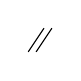
\begin{tikzpicture}[scale=0.2, baseline={([yshift=-0.5ex]current bounding box.center)}]  
			\draw[thin] (0,0) -- (1,1.5);  
			\draw[thin] (0.5,0) -- (1.5,1.5);  
		\end{tikzpicture}%  
	}%  
}  
\newcommand{\fourch}[4]
{\\[3pt]
	\begin{tabular}
		{*{4}{@{}p{4cm}}}
		A.~#1 & B.~#2 & C.~#3 & D.~#4
	\end{tabular}	
}
\newcommand{\fourchh}[4]
{\\[5pt]
	\begin{tabular}
		{*{4}{@{}p{20cm}}}
		A.~#1 \\[5pt] B.~#2 \\[5pt] C.~#3 \\[5pt] D.~#4
	\end{tabular}	
}
\newcommand{\fourchhh}[4]
{\\[3pt]
	\begin{tabular}
		{*{4}{@{}p{7.5cm}}}
		A.~#1 & B.~#2 \\[2pt] C.~#3 & D.~#4
	\end{tabular}	
}
\newcommand{\independent}{\perp\!\!\!\perp}
\everymath{\displaystyle}
\allowdisplaybreaks




\begin{document}
\tdplotsetmaincoords{70}{110} 
\pagestyle{fancy}
\lhead{Lecture 2}
\chead{illusion \& FzRainD}
\rhead{\today}

\setcounter{section}{1}
\section{可逆矩阵和行列式}

进入 \S 2 节,我们本节的任务主要是延续上节的讨论,探寻对方阵而言,什么样的方阵能在 \( \F\n \) 中可逆. 进一步,如果 \( A \) 可逆,那么解线性方程组 \( AX=\beta \) 就变得非常容易了,只需要 \( X=A^{-1}AX=A^{-1}\beta \). 我们离这种 \( n \) 个方程组成的关于 \( n \) 个变元的线性方程组的公式解,只有一步之遥,那就是如何给出 \( A^{-1} \) 的表达式?
但这些假设的前提是,我们已经知道矩阵 \( A \) 可逆,当务之急应该是找出一个判定 \( A \) 可逆的法则. 

\subsection{序幕: 可逆矩阵和一般线性群}
\begin{definition}[可逆矩阵]\label{2.1.1}
	设 \( A \in \F\n \),称 \( A \) 是可逆矩阵,若存在 \( B \in \F\n \) 使得 \( AB=BA=E_n \). 此时,一般记 \( B=A^{-1} \). 从定义可见,可逆矩阵与矩阵本身互为逆矩阵,即 \( A^{-1} \) 的逆矩阵也为 \( A \).
	
\end{definition}

\begin{property}[可逆矩阵的性质]\label{2.1.2}
	若矩阵 \( A, B \in \F\n \) 可逆,那么
	\begin{enumerate}[(1)]
		\item 矩阵 \( A \) 的逆元 \( B=A^{-1} \) 必定唯一;
		\item (穿脱法则 I) \ 矩阵 \( AB \) 也可逆,其逆元 \( (AB)^{-1}=B^{-1}A^{-1} \);
		\item (穿脱法则 II) \ 对一列方阵 \( \{A_k\}_{1 \leq k \leq n} \) 为可逆矩阵,那么 \( A_1A_2\cdots A_n \) 也可逆,且 \( (A_1A_2\cdots A_n)^{-1}=A_n^{-1}A_{n-1}^{-1}\cdots A_1^{-1} \);
		\item (转置与取逆的协调) \ \( A\T \) 也可逆,且 \( (A\T)^{-1}=(A^{-1})\T \).
	\end{enumerate}
	
\end{property}

\begin{proof}
	(1) 设还有 \( C \in \F\n \) 使得 \( AC=CA=E_n \). 那么 \( C=E_nC=(BA)C=B(AC)=BE_n=B \). (2) 只需要验证定义,\( (B^{-1}A^{-1})(AB)=B^{-1}(A^{-1}A)B=B^{-1}E_nB=B^{-1}B=E_n \). 另一方面,\( (AB)(B^{-1}A^{-1})=E_n \) 是类似的. (3) 完全等同 (2),只需要用归纳法. (4) 验证 \( (A^{-1})\T(A\T)=(AA^{-1})\T=E_n\T=E_n \). 同理 \( (A\T)(A^{-1})\T= E_n \).
\end{proof}

\begin{example}[初等矩阵]	\label{2.1.3}
	初等矩阵均可逆. 且它们的逆矩阵十分容易求出. 可以自行验证如下的结论:
	\[ E(i,j(c))^{-1}=E(i,j(-c)), \; E(i(c))^{-1}=E(i(c^{-1})) \ (c \neq 0), \; E(i,j)^{-1}=E(i,j). \]
	现在我们明白了,所谓初等矩阵对应操作的逆操作,无非就是左乘初等矩阵的逆矩阵.

\end{example}

\begin{example}[单位矩阵]
	单位矩阵显然可逆,且 \( E_n^{-1}=E_n \).
\end{example}

\begin{example}\label{2.1.5}
	若矩阵 \( A,B \) 可逆,那么 \( A+B \) 不一定可逆,例如取 \( A=E_n, \; B=-E_n \),那么 \( A+B=O \). 而必定不存在矩阵 \( C \in \F\n \) 使得 \( CO=OC=E_n \)!
	
\end{example}

事实上,在性质 \ref{2.1.2} 的证明中我们只用到了矩阵乘法的结合律,矩阵乘法存在幺元,以及可逆矩阵的定义,即定义 \ref{2.1.1}. 这提示我们性质 \ref{2.1.2} 应该具有一般性. 接下来,我们将矩阵环 \( \F\n \) 的乘法部分作如下提炼,就得到群的定义.

\begin{definition}[群]
	设 \( G \) 是一个非空集合,其上存在一个二元运算 \( \cdot: G \times G \to G \),满足
	\begin{enumerate}
		\item[(1)] \textbf{结合律} \( (ab)c=a(bc) \);
	\end{enumerate}
	那么称 \( (G,\cdot) \) 为一个半群,进一步,如果还有
	\begin{enumerate}
		\item[(2)] \textbf{幺元性质} 存在 \( e \in G \) 使得 \( ae=ea=a \);
	\end{enumerate}
	那么称 \( (G,\cdot) \) 为一个幺半群. 进一步,如果还有
	\begin{enumerate}
		\item[(3)] \textbf{存在逆元} 对 \( a \in G \),存在 \( a^{-1} \in G \) 使得 \( a(a^{-1})=(a^{-1})a=e \);
	\end{enumerate}
	\textbf{那么称 \( (G,\cdot) \) 为一个群. } 进一步,如果还有
	\begin{enumerate}
		\item[(4)] \textbf{交换律} \( ab=ba \).
	\end{enumerate}
	那么称 \( (G,\cdot) \) 为一个交换群或者 Abel 群. 上述定义中,\( a,b,c \in G \) 都是任取的.
\end{definition}

上述定义我们一点都不陌生,我们可以很清楚地发现,环和域的定义几乎完全就是满足上述定义的两种运算的拼接,并额外满足两种运算的协调性而已. 轻而易举地获得下面的例子.

\begin{example}
	设 \( \F \) 是域,那么 \( (\F,+) \) 在数的通常加法下为一个 Abel 群,记 \( \F^*:=\F \textbackslash \{0\} \),那么 \( (\F^*,\cdot) \) 在数的通常乘法下为一个 Abel 群. 
\end{example}

\begin{example}
	设 \( \F\n \) 是域 \( \F \) 上的全矩阵环,那么 \( (\F\n,+) \) 在通常矩阵的加法下为一个 Abel 群. 
\end{example}

\begin{example}
	记 \( \gf:=\{ A \in \F\n \mid \exists \ B \in \F\n, \; AB=BA=E_n \} \),也就是 \( \F\n \) 中的可逆矩阵全体. 那么 \( (\gf,\cdot) \) 在配备通常矩阵的乘法下为一个群,但是由于对于 \( n \geq 2 \),矩阵乘法一般不具备交换律,那么是一个非 Abel 群. 当 \( n=1 \) 时,显然 \( \text{GL}_1(\mathbb{F})= \F^* \),那么 \( (\text{GL}_1(\mathbb{F}),\cdot) \) 为一个 Abel 群. 
	
	一般称 \( (\gf,\cdot) \) 为域 \( \F \) 上的 \( n \) 级一般线性群. 注意 \( (\gf,+) \) 不是一个群,因为例 \ref{2.1.5} 告诉我们可逆矩阵全体对加法不封闭,因此不构成二元运算.
\end{example}

\begin{property}[群的性质]
	设 \( (G,\cdot) \) 为群,任取 \( a,b \in G \),那么
	\begin{enumerate}
		\item \( e \in G \) 唯一,即群中幺元唯一;
		\item \( a^{-1} \in G \) 唯一,即群中任意元素的可逆元唯一;
		\item (穿脱法则 I) \( (ab)^{-1}=b^{-1}a^{-1} \);
		\item (穿脱法则 II) 任取 \( a_1,\cdots,a_n \in G \),那么 \( (a_1a_2\cdots a_n)^{-1}=a_n^{-1}a_{n-1}^{-1}\cdots a_1^{-1} \).
	\end{enumerate}
\end{property}

\begin{proof}
	\( (2)-(4) \) 直接照搬性质 \ref{2.1.2} 的证明即可,对 \( (1) \) 注意到如存在 \( e_1 \neq e_2 \in G \) 为幺元,那么 \( e_1,e_2 \) 均为 \( e_1 \) 的幺元,而幺元唯一.
\end{proof}

下面的命题说明了可逆矩阵只能在方阵中定义,而无法推广到一般的矩阵. 

\begin{proposition}\label{2.1.11}
	对 \( n \neq m \),不存在 \( A \in \F\nm \) 以及 \( B \in \F\mn \) 使得 \( AB= E_n, \; BA=E_m \).
	
\end{proposition}

\begin{proof}
	(\textbf{法一}) \ 利用迹的性质即可,注意到若结论不然,那么 \(\tr(AB)=n \neq m=\tr(BA) \).
	
	\vspace{1ex}
	
	(\textbf{法二}) \ 不妨设 \( m>n \). 若结论不然,断言线性方程组 \( AX=O \) 只有零解. 首先 \( X=O \) 显然为解. 其次,对任意满足方程的 \( X_1 \in \F^m \) 使得 \( AX_1=O \leadsto X_1=BAX_1=BO=O \). 设 \( PA\T=K \),其中 \( P \) 为若干 \( m \) 阶矩阵的乘积,对 \( A\T \) 施行初等行变换,使其变为简化行阶梯形矩阵 \( K \). 那么非零行数目 \( r(A\T) \leq \min\{n,m\}=n<m \). 故 \( PA\T=K \) 的第 \( m \) 行必定为零行. 即 \( \varepsilon_m^T K= O_{1 \times n}= \varepsilon_m^T PA\T \). 两边同时取转置,有 \( A(P\T\varepsilon_m)=O_{n \times 1} \). 故只能 \( P\T\varepsilon_m=O \). 利用性质 \ref{2.1.2} (3),初等矩阵都为可逆矩阵,故若干初等矩阵的积也为可逆矩阵,那么由性质 \ref{2.1.2} (4) 可知 \( P\T \) 可逆,对  \( P\T\varepsilon_m=O \) 两边同乘 \( P\T \) 的逆得到 \( \varepsilon_m=O \) 矛盾.
\end{proof}

为了进一步研究可逆矩阵的判定条件,我们先对可逆矩阵有一个初步刻画.

\begin{proposition}[可逆的必要条件]\label{2.1.12}
	设 \( A \in \gf \),即定义 \ref{2.1.1},存在矩阵 \( B \in \F\n \),使得 \( BA=AB=E_n \),其中 \( B \) 当然也是可逆的. 那么
	\begin{enumerate}[(1)]
		\item 线性方程组 \( AX=O \) 仅有零解;
		\item \( A \) 的简化行阶梯形矩阵为 \( E_n \) 或者简化行阶梯形矩阵的非零行数目 \( r(A)=n \);
		\item \( A \) 可以只经过初等行变换或者初等列变换变为 \( E_n \);
		\item \( A \) 可以表示为初等矩阵的乘积.
	\end{enumerate}
	
\end{proposition}

\begin{proof}
	(1) 首先 \( X=O \) 显然为解. 其次,对每个满足线性方程组 \( AX=O \) 的解都有 \( X=A^{-1}AX=A^{-1}O=O \);
	(2) 否则,设 \( A \) 的简化行阶梯矩阵为 \( K=PA \),其中 \( P \) 为若干初等矩阵之积,为可逆矩阵. 设 \( K \) 的非零行数目 \( r(A)<n \). 即 \( \varepsilon_n\T K=O= \varepsilon_n\T PA \),那么 \( A\T(P\T \varepsilon_n)=O \). 然而由性质 \ref{2.1.2} (4) \( P\T \) 可逆,这意味着 \( P\T \varepsilon_n \neq O \). 那么 \( A\T X=O \) 存在非零解,但 \( A\T \) 可逆,矛盾. (1)(2) 事实上完全是命题 \ref{2.1.11} 法二过程的照搬.
	
	\vspace{1ex}
	
    (3) 只经过初等行变换是显然的,对初等列变换,考察 \( A\T \),由于 \( A\T \) 可以只经过初等行变换化为 \( E_n \),这就对应 \( A \) 可以只经过初等列变换化为 \( E_n \). (4) 由 (3) 立即得到.
\end{proof}

\begin{corollary}	\label{2.1.13}
	设 \( A \in \F\n \),那么 \( A \in \gf \) 的充分必要条件为 \( A \) 可以表示为初等矩阵的乘积.

\end{corollary}

\begin{proof}
	用命题 \ref{2.1.12} 和例 \ref{2.1.3} 即可.
\end{proof}

\subsection{代数动机: 线性方程组的公式解}

\subsubsection{行列式的归纳定义}
为了研究可逆矩阵的判定条件,不妨假设 \( A \) 可逆,那么我们从 \( AX=\beta \) 的解的表达式开始研究,因为我们知道此时 \( X=A^{-1}\beta \) 就是解的表达式. 其中必定会有一些和 \( A^{-1} \) 有关的量. 从二元线性方程组开始,考察
\[ \left\{ \begin{array}{l}
	a_{11}x_1+a_{12}x_2=b_1, \\
	a_{21}x_1+a_{22}x_2=b_2.
\end{array}\right. \leadsto \overline{A}=\begin{bmatrix}
 a_{11} & a_{12} & b_1 \\
 a_{21} & a_{22} & b_2
\end{bmatrix}. \]

由命题 \ref{2.1.12} (2),对 \( \overline{A} \) 实行 Guass-Jordan 消元法必定能得到两个主元,不妨考虑简单情形,也就是适当调整 \( A \) 使得操作过程无须涉及行的互换变换. 在这个假定下,\( a_{11} \neq 0 \),也就是不考虑 \( a_{11}=0, a_{21} \neq 0 \),然后将第 2 行换到第 1 行. 那么
\[ \begin{bmatrix}
	a_{11} & a_{12} & b_1 \\
	a_{21} & a_{22} & b_2
\end{bmatrix} \leadsto \begin{bmatrix}
1 & a_{12}/a_{11} & b_1/a_{11} \\
a_{21} & a_{22} & b_2
\end{bmatrix} \leadsto \begin{bmatrix}
1 & \frac{a_{12}}{a_{11}} & \frac{b_1}{a_{11}} \\[2ex]
0 & a_{22} - \frac{a_{21} a_{12}}{a_{11}} & b_2 - \frac{a_{21} b_1}{a_{11}}
\end{bmatrix}. \]

此时必定有 \( a_{22}a_{11} \neq a_{21} a_{12} \),否则对 \( A \) 实行初等行变换得不到两个主元,与可逆前提矛盾. 那么
\[ \begin{bmatrix}
	1 & \frac{a_{12}}{a_{11}} & \frac{b_1}{a_{11}} \\[2ex]
	0 & a_{22} - \frac{a_{21} a_{12}}{a_{11}} & b_2 - \frac{a_{21} b_1}{a_{11}}
\end{bmatrix} \leadsto \begin{bmatrix}
1 & \frac{a_{12}}{a_{11}} & \frac{b_1}{a_{11}} \\[2ex]
0 & a_{22}a_{11} - a_{21} a_{12} & a_{11} b_2 - a_{21} b_1
\end{bmatrix} \leadsto \begin{bmatrix}
1 & \frac{a_{12}}{a_{11}} & \frac{b_1}{a_{11}} \\[2ex]
0 & 1 & \frac{a_{11} b_2 - a_{21} b_1}{a_{22}a_{11} - a_{21} a_{12}}
\end{bmatrix}. \]

进一步变为简化行阶梯形矩阵
\[ \begin{bmatrix}
	1 & \frac{a_{12}}{a_{11}} & \frac{b_1}{a_{11}} \\[2ex]
	0 & 1 & \frac{a_{11} b_2 - a_{21} b_1}{a_{22}a_{11} - a_{21} a_{12}}
\end{bmatrix} \to \begin{bmatrix}
1 & 0 & \frac{a_{12} b_2 - a_{22} b_1}{a_{22}a_{11} - a_{21} a_{12}} \\[2ex]
0 & 1 & \frac{a_{11} b_2 - a_{21} b_1}{a_{22}a_{11} - a_{21} a_{12}}
\end{bmatrix}. \]

引入记号
\[ \det A=\begin{vmatrix}
	a_{11} & a_{12} \\ a_{21} & a_{22}
\end{vmatrix}:= a_{11}a_{22}-a_{12}a_{21}=a_{11}\cdot (-1)^{1+1}a_{12}+a_{21} \cdot (-1)^{1+2}a_{12}. \]

那么上述方程的解即
\[ x_1=\frac{\begin{vmatrix}
		b_1 & a_{12} \\ b_2 & a_{22}
\end{vmatrix}}{\begin{vmatrix}
		a_{11} & a_{12} \\ a_{21} & a_{22}
\end{vmatrix}}, \; x_2=\frac{\begin{vmatrix}
a_{11} & b_1 \\ a_{12} & b_2
\end{vmatrix}}{\begin{vmatrix}
a_{11} & a_{12} \\ a_{21} & a_{22}
\end{vmatrix}}. \]

显然为了使得上述表达式成立,在操作过程我们用到了 \( \det A \neq 0 \). 而对于解的分子,都是和 \( \beta \) 的信息混合在一起,难以提取有关 \( A^{-1} \) 存在的必要信息. 但这只给出了一个大概方向,如何定义更高阶矩阵 \( A \) 的 \(  \det A \) 呢? 进一步,如果定义好了 \( \det A \) 并且发现 \( \det A \neq 0 \),真的能推出矩阵可逆吗? 为了找到一个合适的定义,接着考察三元线性方程组,

\[ \left\{ \begin{array}{l}
	a_{11}x_1+a_{12}x_2+a_{13}x_3=b_1, \\
	a_{21}x_1+a_{22}x_2+a_{23}x_3=b_2, \\
	a_{31}x_1+a_{32}x_2+a_{33}x_3=b_3.
\end{array}\right. \leadsto \overline{A}=\begin{bmatrix}
	a_{11} & a_{12} & a_{13} & b_1 \\
	a_{21} & a_{22} & a_{23} & b_2 \\
	a_{31} & a_{32} & a_{33} & b_3 
\end{bmatrix}. \]

一开始仍然不妨设 \( a_{11} \neq 0 \),那么
\[ \overline{A} \leadsto  \begin{bmatrix}
	1 & a_{12}/a_{11} & a_{13}/a_{11} & b_1/a_{11} \\[2ex]
	0 & a_{22}-\frac{a_{21}a_{12}}{a_{11}} & a_{23}-\frac{a_{21}a_{13}}{a_{11}} & b_2-\frac{b_1a_{12}}{a_{11}} \\[2ex]
	0 & a_{32}-\frac{a_{31}a_{12}}{a_{11}} & a_{33}-\frac{a_{31}a_{13}}{a_{11}} & b_3-\frac{b_1a_{12}}{a_{11}}
\end{bmatrix} \leadsto \begin{bmatrix}
1 & a_{12}/a_{11} & a_{13}/a_{11} & b_1/a_{11} \\[2ex]
0 & a_{22} a_{11} - a_{21} a_{12} & a_{23} a_{11} - a_{21} a_{13} & b_2 a_{11} - b_1 a_{21} \\[2ex]
0 & a_{32} a_{11} - a_{31} a_{12} & a_{33} a_{11} - a_{31} a_{13} & b_3 a_{11} - b_1 a_{31}
\end{bmatrix}. \]

那么子矩阵
\[ \begin{bmatrix}
	a_{22} a_{11} - a_{21} a_{12} & a_{23} a_{11} - a_{21} a_{13} & b_2 a_{11} - b_1 a_{21} \\[2ex]
	 a_{32} a_{11} - a_{31} a_{12} & a_{33} a_{11} - a_{31} a_{13} & b_3 a_{11} - b_1 a_{31}
\end{bmatrix} \]

的简化行阶梯矩阵具有两个主元,将其看成二元线性方程组,由前述,得到解的表达式
\[ x_2=\frac{\begin{vmatrix}
		b_2 a_{11} - b_1 a_{21} & a_{23} a_{11} - a_{21} a_{13} \\ b_3 a_{11} - b_1 a_{31} & a_{33} a_{11} - a_{31} a_{13}
\end{vmatrix}}{\begin{vmatrix}
		a_{22} a_{11} - a_{21} a_{12} & a_{23} a_{11} - a_{21} a_{13} \\ a_{32} a_{11} - a_{31} a_{12} & a_{33} a_{11} - a_{31} a_{13}
\end{vmatrix}}, \; x_3=\frac{\begin{vmatrix}
		a_{22} a_{11} - a_{21} a_{12} & b_2 a_{11} - b_1 a_{21} \\ a_{32} a_{11} - a_{31} a_{12} & b_3 a_{11} - b_1 a_{31}
\end{vmatrix}}{\begin{vmatrix}
a_{22} a_{11} - a_{21} a_{12} & a_{23} a_{11} - a_{21} a_{13} \\ a_{32} a_{11} - a_{31} a_{12} & a_{33} a_{11} - a_{31} a_{13}
\end{vmatrix}}. \]

先化简上式的分母,得到
\begin{align*}
	& \quad \begin{vmatrix}
		a_{11} {\color{teal} a_{22}} - a_{21} {\color{violet} a_{12}} & a_{23} a_{11} - a_{21} a_{13} \\
		{\color{cyan!40!black} a_{32}} a_{11} - a_{31} {\color{violet} a_{12}} & a_{33} a_{11} - a_{31} a_{13}
	\end{vmatrix} \\[1ex]
	&= ({\color{teal} a_{22}} a_{11} - a_{21} {\color{violet} a_{12}})(a_{33} a_{11} - a_{31} a_{13}) - (a_{23} a_{11} - a_{21} a_{13})({\color{cyan!40!black} a_{32}} a_{11} - a_{31} {\color{violet} a_{12}}) \\[1ex]
	&= a_{11}(\, a_{11} a_{33} {\color{teal} a_{22}}- a_{11} {\color{cyan!40!black} a_{32}} a_{23}  + a_{21} a_{13} {\color{cyan!40!black} a_{32}} - a_{21} {\color{violet} a_{12}} a_{33} + a_{31} a_{23} {\color{violet} a_{12}} - a_{31} a_{13}  {\color{teal} a_{22}}   \,) \\[1ex]
	&= a_{11} \left( a_{11} \begin{vmatrix}
{\color{teal} a_{22}} & a_{23} \\
{\color{cyan!40!black} a_{32}} & a_{33}
	\end{vmatrix}
	- a_{21} \begin{vmatrix}
		{\color{violet} a_{12}} & a_{13} \\
		{\color{cyan!40!black} a_{32}} & a_{33} 
	\end{vmatrix}
	+ a_{31} \begin{vmatrix}
		{\color{violet} a_{12}} & a_{13} \\
		{\color{teal} a_{22}} & a_{23} 
	\end{vmatrix} \right)
\end{align*}

类似化简 \( x_2 \) 的分子,
\begin{align*}
	& \quad \begin{vmatrix}
		{\color{teal} b_2} a_{11} - {\color{violet} b_1} a_{21} & a_{23} a_{11} - a_{21} a_{13} \\
		{\color{cyan!40!black} b_3} a_{11} - {\color{violet} b_1} a_{31} & a_{33} a_{11} - a_{31} a_{13}
	\end{vmatrix} \\[1ex]
	&= ({\color{teal} b_2} a_{11} - {\color{violet} b_1} a_{21})(a_{33} a_{11} - a_{31} a_{13}) - ({\color{cyan!40!black} b_3} a_{11} - {\color{violet} b_1} a_{31})({\color{cyan!40!black} a_{32}} a_{11} - a_{31} {\color{violet} a_{12}}) \\[1ex]
	&= a_{11}(\, a_{11} a_{33} {\color{teal} b_2}- a_{11} {\color{cyan!40!black} b_{3}} a_{23}  + a_{21} a_{13} {\color{cyan!40!black} b_{3}} - a_{21} {\color{violet} b_{1}} a_{33} + a_{31} a_{23} {\color{violet} b_{1}} - a_{31} a_{13}  {\color{teal} b_{2}} \,) \\[1ex]
	&= a_{11} \left( a_{11} \begin{vmatrix}
		{\color{teal} b_{2}} & a_{23} \\
		{\color{cyan!40!black} b_{3}} & a_{33}
	\end{vmatrix}
	- a_{21} \begin{vmatrix}
		{\color{violet} b_{1}} & a_{13} \\
		{\color{cyan!40!black} b_{3}} & a_{33} 
	\end{vmatrix}
	+ a_{31} \begin{vmatrix}
		{\color{violet} b_{1}} & a_{13} \\
		{\color{teal} b_{2}} & a_{23} 
	\end{vmatrix} \right)
\end{align*}

注意观察,我们对分子其实无需展开计算,只需要进行替换 \( {\color{violet} a_{12} \leadsto b_1}, \; {\color{teal} a_{22} \leadsto b_2}, \; {\color{cyan!40!black} a_{23} \leadsto b_3} \) 即可. 这事实上就是我们在本节最后叙述的 Cramer 法则. 定义

\begin{align*}
	\det A &=\begin{vmatrix}
		a_{11} & a_{12} & a_{13} \\
		a_{21} & a_{22} & a_{23} \\
		a_{31} & a_{32} & a_{33} 
	\end{vmatrix}:=a_{11} \begin{vmatrix}
		a_{22} & a_{23} \\
		a_{32} & a_{33}
	\end{vmatrix}
	- a_{21} \begin{vmatrix}
		a_{12} & a_{13} \\
		a_{32} & a_{33} 
	\end{vmatrix}
	+ a_{31} \begin{vmatrix}
		a_{12} & a_{13} \\
		a_{22} & a_{23} 
	\end{vmatrix} \\
	&= (-1)^{1+1}a_{11} \begin{vmatrix}
		a_{22} & a_{23} \\
		a_{32} & a_{33}
	\end{vmatrix}
	+(-1)^{2+1} a_{21} \begin{vmatrix}
		a_{12} & a_{13} \\
		a_{32} & a_{33} 
	\end{vmatrix}
	+(-1)^{3+1}a_{31} \begin{vmatrix}
		a_{12} & a_{13} \\
		a_{22} & a_{23} 
	\end{vmatrix}
\end{align*}


那么
\[ x_2= \frac{\begin{vmatrix}
		a_{11} & b_1 & a_{13} \\
		a_{21} & b_2 & a_{23} \\
		a_{31} & b_3 & a_{33} 
\end{vmatrix}}{\begin{vmatrix}
		a_{11} & a_{12} & a_{13} \\
		a_{21} & a_{22} & a_{23} \\
		a_{31} & a_{32} & a_{33} 
\end{vmatrix}}, \; x_3=\frac{\begin{vmatrix}
a_{11} & a_{12} & b_1 \\
a_{21} & a_{22} & b_2 \\
a_{31} & a_{32} & b_3 
\end{vmatrix}}{\begin{vmatrix}
a_{11} & a_{12} & a_{13} \\
a_{21} & a_{22} & a_{23} \\
a_{31} & a_{32} & a_{33} 
\end{vmatrix}}. \]

带回 \( x_1+(a_{12}/a_{11})x_2+(a_{13}/a_{11}) x_3=b_1/a_{11} \),经过计算可以得到类似的结果,即
\[ x_1=\frac{\begin{vmatrix}
		b_{1} & a_{12} & a_{13} \\
		b_{2} & a_{22} & a_{23} \\
		b_{3} & a_{32} & a_{33} 
\end{vmatrix}}{\begin{vmatrix}
		a_{11} & a_{12} & a_{13} \\
		a_{21} & a_{22} & a_{23} \\
		a_{31} & a_{32} & a_{33} 
\end{vmatrix}}. \]

于是我们下面提出行列式的第一种定义,按列展开的数学归纳法定义.

\begin{definition}[行列式的归纳定义]\label{2.2.1}
	考虑 \( A \in \F\n \),现在递归定义 \( \det A \ (|A|): \F\n \to \F \). 当 \( n=1 \) 时,设 \( A=(a) \),定义 \( \det A=a \). 现在假设 \( n-1 \) 阶的行列式已经定义好,设元素 \( a_{ij} \) 的余子式为从 \( A \) 中删去第 \( i \) 行和第 \( j \) 列所得 \( n-1 \) 阶矩阵的行列式,记作 \( M_{ij} \),即
	\[ M_{ij}=\det \begin{bmatrix}
		a_{11} & \cdots & a_{1,j-1} & a_{1,j+1} & \cdots & a_{1n} \\
		\vdots &        & \vdots   & \vdots   &        & \vdots \\
		a_{i-1,1} & \cdots & a_{i-1,j-1} & a_{i-1,j+1} & \cdots & a_{i-1,n} \\
		a_{i+1,1} & \cdots & a_{i+1,j-1} & a_{i+1,j+1} & \cdots & a_{i+1,n} \\
		\vdots &        & \vdots   & \vdots   &        & \vdots \\
		a_{n1} & \cdots & a_{n,j-1} & a_{n,j+1} & \cdots & a_{nn}
	\end{bmatrix}. \]
	
	记元素 \( a_{ij} \) 的代数余子式为 \( A_{ij}:=(-1)^{i+j}M_{ij} \).那么 \( \det A=|A|:= a_{11}A_{11}+a_{21}A_{21}+\cdots+a_{n1}A_{n1} \). 这一定义称为按第一列展开归纳定义. 对 \( n=0 \) 的情形,规定 \( \det A=1 \).
	
\end{definition}

\subsubsection{行列式的基本性质}

这个定义是否有用,还需要看它能不能用来解决我们先前的问题: 即可逆矩阵的判定以及线性方程组的公式解. 那么沿着定义,我们第一步自然是刻画一些相关的性质.

\begin{property}[行列式的性质] \phantomsection \label{2.2.2} 
	在定义 \ref{2.2.1} 的基础上,将矩阵按列分块,得到 \( A=(\alpha_1,\alpha_2,\cdots,\alpha_n) \),也记行列式 \( \det A=\det(\alpha_1,\alpha_2,\cdots,\alpha_n) \). 任取 \( \beta \in \F^n \) 以及 \( c \in \F \),那么
	\begin{enumerate}[(1)]
		\item 将 \( \det A \) 的一列乘以某个常数 \( c \) 得到 \( \det B \),那么 \( \det B=c\det A \). 即 \( \det(\alpha_1,\cdots,\alpha_{i-1},c\alpha_i,\alpha_{i+1},\cdots,\alpha_n)=c\det A \),进而 \( \det(cA)=c^n \det A \);
		\item 一般没有 \( \det(A+B)=\det A+\det B \),但是有 \( \det(\alpha_1,\cdots,\alpha_{i-1},\alpha_i+\beta,\alpha_{i+1},\cdots,\alpha_n)=\det(\alpha_1,\alpha_2,\cdots,\alpha_n)+\det(\alpha_1,\cdots,\alpha_{i-1},\beta,\alpha_{i+1},\cdots,\alpha_n) \);
		\item 交换行列式的两列,行列式改变符号,即 \( \det(\cdots,\alpha_{i-1},\alpha_j,\alpha_{i+1},\cdots,\alpha_{j-1},\alpha_i,\alpha_{j+1},\cdots)=-\det A \ (i<j) \).
	    \item 对矩阵 \( A \) 的列作倍法变换,行列式的值不变. 即将行列式的一列乘以常数 \( c \) 加到另一列上,行列式的值不变.
	    \[ \det(\cdots,\alpha_{i-1},\alpha_i+c\alpha_j,\alpha_{i+1},\cdots,\alpha_{j-1},\alpha_j,\alpha_{j+1},\cdots)=\det A. \]
	    \item \( \det A \) 可以按第 \( r \ (1\leq r \leq n) \) 列展开,即
	    \[ \det A= a_{1r}A_{1r}+a_{2r}A_{2r}+\cdots+a_{nr}A_{nr}. \]
	    \item 转置不改变行列式的值,即 \( \det A\T= \det A \).
	\end{enumerate}
\end{property}

\begin{proof}
     (1)(2) 用归纳法是非常容易的. 现考虑 (3). 用数学归纳法,若交换的是非第一列的两列即证. 现在考虑若交换的是第一列和第二列的情况,设 \( A \) 经过该交换得到矩阵 \( B \). 记矩阵 \( A,B \) 的余子式为 \( M_{ij}, \; N_{ij} \). 自然有 \( M_{i2}=N_{i1} \). 将 \( \det B \) 按第一列展开
     \[ \det B= \sum_{i=1}^{n} (-1)^{i+1} b_{i1}N_{i1}= \sum_{i=1}^{n} (-1)^{i+1} a_{i2}M_{i2}= -\sum_{i=1}^{n} (-1)^{i+2} a_{i2}M_{i2}. \]
     
     现在只要证明 \( \det A \) 能按第二列展开即可. 设矩阵 \( A \) 删去第 \( i,k \) 行以及 \( 1,2 \) 列余下矩阵的行列式为 \( M\begin{bmatrix}
     i & k \\ 1 & 2
     \end{bmatrix} \).
     
     利用定义 \ref{2.2.1} 有
     \begin{align*}
     	\det A & = \sum_{i=1}^{n} (-1)^{i+1}a_{i1}M_{i1} \\
     	&= \sum_{i=1}^{n} (-1)^{i+1}a_{i1} \left(\sum_{k=1}^{i-1}a_{k2}(-1)^{k+1}M\begin{bmatrix}
     		i & k \\ 1 & 2
     	\end{bmatrix}+\sum_{k=i+1}^{n}a_{k2}(-1)^{(k-1)+1}M\begin{bmatrix}
     	i & k \\ 1 & 2
     	\end{bmatrix} \right) \\
     	&= \sum_{1 \leq k<i \leq n}^{} (-1)^{i+k} a_{i1}a_{k2} \begin{bmatrix}
     		i & k \\ 1 & 2
     	\end{bmatrix}+ \sum_{1 \leq i<k \leq n}^{}  (-1)^{i+k+1} a_{i1}a_{k2} \begin{bmatrix}
     	i & k \\ 1 & 2
     	\end{bmatrix} \\
     	&= \sum_{k=1}^{n} (-1)^{k+2}a_{k2} \left( \sum_{i=k+1}^{n} (-1)^{i-1+1}a_{i1}M\begin{bmatrix}
     		i & k \\ 1 & 2
     	\end{bmatrix}+ \sum_{i=1}^{k-1}(-1)^{i+1}a_{i1}M\begin{bmatrix}
     	i & k \\ 1 & 2
     	\end{bmatrix} \right) \\
     	&= \sum_{k=1}^{n} (-1)^{k+2}a_{k2}M_{k2}.
     \end{align*}
     
     现在我们已经证明了结论对第 1, 2 列互换以及不含第一列的互换成立. 对第 1, \( k \) 列互换的情形,记 \( (i,j) \) 为第 \( (i,j) \) 列互换的操作,\( (i_2,j_2)(i_1,j_1) \) 这样的复合表示先互换 \( i_1,j_1 \) 列,再互换 \( i_2,j_2 \) 列. 那么 \( (1,k)=(k-1,k)\cdots(3,4)(2,3)(1,2)(2,3)(3,4)\cdots(k-1,k) \). 上述每一次互换都改变一次行列式的符号,一共进行了 \( 2(k-1)+1 \) 次互换,行列式的值自然改变符号.
     
     推论 \ref{2.2.3} 直接来源于 (3). 利用推论 \ref{2.2.3} 以及 (2),又可以得到 (4). (5) 的证明只需要对行列式作互换 \( (1,2)(2,3)(3,4)\cdots(r-1,r) \),然后按第一列展开即可. 为证明 (6),我们先断言若行列式的一行全为零,那么行列式为零,利用归纳假设即得. 然后说明 \( \det A \) 可以按第一行展开,反复利用 (2),
     \begin{align*}
     	\det A= \begin{vmatrix}
     		a_{11} & a_{12} & \cdots & a_{1n} \\
     		a_{21} & a_{22} & \cdots & a_{2n} \\
     		\vdots & \vdots & \ddots & \vdots \\
     		a_{n1} & a_{n2} & \cdots & a_{nn}
     	\end{vmatrix} &=  \begin{vmatrix}
     	a_{11} & a_{12} & \cdots & a_{1n} \\
     	0 & a_{22} & \cdots & a_{2n} \\
     	\vdots & \vdots & \ddots & \vdots \\
     	0 & a_{n2} & \cdots & a_{nn}
     	\end{vmatrix}+ \begin{vmatrix}
     	0 & a_{12} & \cdots & a_{1n} \\
     	a_{21} & a_{22} & \cdots & a_{2n} \\
     	\vdots & \vdots & \ddots & \vdots \\
     	a_{n1} & a_{n2} & \cdots & a_{nn} \\
     \end{vmatrix} \\
     	&= a_{11}A_{11}+\begin{vmatrix}
     		0 & a_{12} & \cdots & a_{1n} \\
     		a_{21} & a_{22} & \cdots & a_{2n} \\
     		\vdots & \vdots & \ddots & \vdots \\
     		a_{n1} & a_{n2} & \cdots & a_{nn} \\
     	\end{vmatrix} \\
     	&= a_{11}A_{11}+ \begin{vmatrix}
     	0 & a_{12} & \cdots & a_{1n} \\
     	a_{21} & 0 & \cdots & a_{2n} \\
     	\vdots & \vdots & \ddots & \vdots \\
     	a_{n1} & 0 & \cdots & a_{nn} \\
     	\end{vmatrix}+\begin{vmatrix}
     	0 & 0 & \cdots & a_{1n} \\
     	a_{21} & a_{22} & \cdots & a_{2n} \\
     	\vdots & \vdots & \ddots & \vdots \\
     	a_{n1} & a_{n2} & \cdots & a_{nn} \\
     	\end{vmatrix} \\
     	&= a_{11}A_{11}+a_{12}A_{12}+\cdots \\
     	&=  a_{11}A_{11}+a_{12}A_{12}+\cdots+a_{1n}A_{1n}+ \begin{vmatrix}
     		0 & 0 & \cdots & 0 \\
     		a_{21} & a_{22} & \cdots & a_{2n} \\
     		\vdots & \vdots & \ddots & \vdots \\
     		a_{n1} & a_{n2} & \cdots & a_{nn} \\
     	\end{vmatrix} \\
     	&= \det A+0.
     \end{align*}
     
     最后对 \( A\T \) 按第一行展开完全等同于对 \( A \) 按第一列展开,即 \( \det A=\det A\T \).
\end{proof}


\begin{corollary}\label{2.2.3}
	若行列式有两列相同,那么行列式的值为 0.
	
\end{corollary}

\begin{proof}
	若 \( \tz \F \neq 2 \),根据性质 \ref{2.2.2} (4),交换这两个相同的列,可以得到 \( \det A=-\det A \),进而 \( 2\det A=0 \) 蕴含 \( \det A=0 \).  \( \tz \F=2 \) 时,由于 \( -1=1 \),那么任意交换行列式的列,行列式的值均不变. 用数学归纳法即可,当 \( n=2 \) 时显然成立,对 \( n>2 \),将两个相同的列调换至第 \( 2 \sim n \) 列,再按第一列展开用归纳假设即可.
\end{proof}

\begin{corollary}	\label{2.2.4}
	利用性质 \ref{2.2.2} (7),可以直接把性质 \ref{2.2.2} 中所有有关列的表述改为行,都完全成立.

\end{corollary}

\begin{corollary}\label{2.2.5}
	若行列式有一行或者一列全为零,那么行列式的值为 0.
	
\end{corollary}

\begin{proof}
	有许多证明方法,例如用性质 \ref{2.2.2} (1) 选择一个非零常数 \( c \) 乘到这一个全为零的行/列 或者性质 \ref{2.2.2} (2) 将 \( 0 \) 拆分为 \( 0+0 \),或者按全为零的列或者行展开,即性质 \ref{2.2.2} (5),还可以把其余任意一行/列加到这一个全为零的行/列,进而用推论 \ref{2.2.3}. 
\end{proof}

\subsubsection{可逆矩阵的判定和 Cramer 法则}

有了性质 \ref{2.2.2} 我们可以得出下面两个重要的命题,进而体会行列式的工具性: 刻画可逆矩阵的充要条件以及给出一类线性方程组的公式解.

\begin{definition}[伴随矩阵]\label{2.2.6}
	设 \( A \in \F\n \),定义矩阵 \( A \) 的古典伴随矩阵为 \( A^*:=(A_{ji}) \),即按正常行列顺序排列 \( a_{ij} \) 的代数余子式,而后转置. 
	
\end{definition}

\begin{proposition}[正交性]	\label{2.2.7}
	在定义 \ref{2.2.6} 的基础上,成立 \( AA^*=A^*A=(\det A)E_n \). 换言之,用矩阵乘法的定义就写出
	\[ a_{1i}A_{1j}+a_{2i}A_{2j}+\cdots+a_{ni}A_{nj}=(\det A)\delta_{ij}, \]
	以及
	\[ a_{i1}A_{j1}+a_{i2}A_{j2}+\cdots+a_{in}A_{jn}=(\det A)\delta_{ij}. \]

\end{proposition}

\begin{proof}
	对 \( i=j \),就是性质 \ref{2.2.2} (5) 和推论 \ref{2.2.4}. 对 \( i \neq j \),不妨 \( i<j \),以第一个式子为例,构造行列式
	\[ \det \bordermatrix{
		& & i & & j &  \cr
		&\cdots & a_{1i} & \cdots & a_{1i} & \cdots \cr
		&\cdots & a_{2i} & \cdots & a_{2i} & \cdots \cr
		&\vdots & \vdots & \ddots & \vdots & \vdots \cr
		&\cdots & a_{ni} & \cdots & a_{ni} & \cdots 
	}= a_{1i}A_{1j}+a_{2i}A_{2j}+\cdots+a_{ni}A_{nj}=0. \]
	
	这里对第 \( j \) 列展开,且运用推论 \ref{2.2.3}.
\end{proof}

\begin{lemma}\label{2.2.8}
	设 \( A \in \F\n, \; B \in \F^{m \times m}, \; C \in  \F\mn \),那么
	\[ \det \begin{bmatrix}
		A & O \\
		C & B
	\end{bmatrix}= \det A \det B. \]
	
\end{lemma}

\begin{proof}
	对 \( n \) 用归纳法. 当 \( n=1 \) 时,按第一行展开立即得到. 设对 \( n-1 \) 命题成立,考虑一般的 \( n \). 为方便讨论,下面 \( M_{ij} \) 表示 \( (i,j) \) 元的余子式对应的矩阵,也表示余子式本身. 那么对原矩阵按第一行展开得到
	\begin{align*}
		\det \begin{bmatrix}
			A & O \\
			C & B
		\end{bmatrix} &= (-1)^{1+1} a_{11} \det \begin{bmatrix}
		M_{11} & O \\
		* & B
		\end{bmatrix}+ (-1)^{1+2} a_{12} \det \begin{bmatrix}
		M_{12} & O \\
		* & B
		\end{bmatrix}+\cdots+ (-1)^{1+n} a_{1n} \det \begin{bmatrix}
		M_{1n} & O \\
		* & B
		\end{bmatrix} \\
		&= \left[\sum_{i=1}^{n} (-1)^{i+1}a_{1i}M_{1i}\right] \det B= \det A \det B.
	\end{align*}
\end{proof}

\begin{proposition}[同态性]\label{2.2.9}
	设 \( A,B \in \F\n \),那么 \( \det(AB)=(\det A)(\det B) \).
	
\end{proposition}

\begin{proof}
	(\textbf{法一})\ 考虑分块矩阵
	\[  \begin{bmatrix}
		A & O \\
		-E & B
	\end{bmatrix}=\begin{bmatrix}
	a_{11} & a_{12} & \cdots & a_{1n} & 0 & 0 & \cdots & 0 \\
	a_{21} & a_{22} & \cdots & a_{2n} & 0 & 0 & \cdots & 0 \\
	\vdots & \vdots & \ddots & \vdots & \vdots & \vdots & \ddots & \vdots \\
	a_{n1} & a_{n2} & \cdots & a_{nn} & 0 & 0 & \cdots & 0 \\
	-1 & 0 & \cdots & 0  & b_{11} & b_{12} & \cdots & b_{1n} \\
    0 & -1 & \cdots & 0  & b_{21} & b_{22} & \cdots & b_{2n} \\
	\vdots & \vdots & \ddots & \vdots & \vdots & \vdots & \ddots & \vdots \\
	0 & 0 & \cdots & -1 & b_{n1} & b_{n2} & \cdots & b_{nn} 
	\end{bmatrix}. \]
	
	我们要做的无非就是用分块初等变换
	\[ \begin{bmatrix}
		A & O \\
		-E & B
	\end{bmatrix} \leadsto \begin{bmatrix}
	A-AE & O+AB \\
	-E & B
	\end{bmatrix} \]
	
	但是这不是简单的初等变换,我们知道只有倍法变换不会改变行列式,那么这样的分块初等变换能变成若干倍法变换的复合吗,试一试就知道了. 现在左乘 \( E(1,2n(a_{1n}))\cdots E(1,n+2(a_{12}))E(1,n+1(a_{11})) \),这样就能将 \( A \) 的第一行全部打成零,那么观察 \( B \) 上方矩阵的第一行,设它的 \( (1,j) \) 元为 \( c_{1j} \). 那么
	\[ c_{1j}= b_{1j}a_{11}+b_{2j}a_{12}+\cdots+b_{nj}a_{1n}=(AB)_{1j}. \]
	
	类似的方法,接下来依次干掉 \( A \) 的 \( 2\sim n \) 行,就完成了前述分块初等变换的作用,那么事实上也就得到了分块倍法变换也就是若干倍法变换的复合. 我们依旧记 \( B \) 上方矩阵的 \( (i,j) \) 元为 \( c_{ij} \). 利用倍法变换不改变行列式的值,那么
	\[ \det \begin{bmatrix}
		A & O \\
		-E & B
	\end{bmatrix}= \det \begin{bmatrix}
	 0 & 0 & \cdots & 0 & c_{11} & c_{12} & \cdots & c_{1n} \\
	 0 & 0 & \cdots & 0 & c_{21} & c_{22} & \cdots & c_{2n} \\
	\vdots & \vdots & \ddots & \vdots & \vdots & \vdots & \ddots & \vdots \\
	  0 & 0 & \cdots & 0 & c_{n1} & c_{n2} & \cdots & c_{nn} \\
	-1 & 0 & \cdots & 0  & b_{11} & b_{12} & \cdots & b_{1n} \\
	0 & -1 & \cdots & 0  & b_{21} & b_{22} & \cdots & b_{2n} \\
	\vdots & \vdots & \ddots & \vdots & \vdots & \vdots & \ddots & \vdots \\
	0 & 0 & \cdots & -1 & b_{n1} & b_{n2} & \cdots & b_{nn} 
	\end{bmatrix}. \]
	
	由引理 \ref{2.2.8},左端也就是 \( \det A \det B \). 对右端按第一列展开,发现只剩下 \( (-1)^{(n+1)+1} \cdot (-1) M_{n+1,1} \). 再对 \( M_{n+1,1} \) 按第一列展开,又只剩下 \( (-1)^{(n+1)+1} \cdot (-1) M'_{n+1,1} \). 这样不断进行下去第 \( n \) 次展开只剩下 \( (-1)^{(n+1)+1} \cdot (-1) \det (AB) \). 综合起来就有
	\[ (\det A)(\det B)=(-1)^{n(n+1)+2(1+\cdots+1)} \cdot \det (AB)= (-1)^{2n(n+1)} \det (AB)= \det(AB). \]
	
	另一种思路求解右端行列式,对其进行列的对换,实行 \( (1,n+1)(2,n+2)\cdots(n,2n) \) 后,原行列式变为
	\[ \begin{bmatrix}
		c_{11} & c_{12} & \cdots & c_{1n} & 0 & 0 & \cdots & 0 \\
		c_{21} & c_{22} & \cdots & c_{2n} & 0 & 0 & \cdots & 0 \\
		\vdots & \vdots & \ddots & \vdots & \vdots & \vdots & \ddots & \vdots \\
		c_{n1} & c_{n2} & \cdots & c_{nn} & 0 & 0 & \cdots & 0 \\
		b_{11} & b_{12} & \cdots & b_{1n} & -1 & 0 & \cdots & 0 \\
		b_{21} & b_{22} & \cdots & b_{2n} & 0 & -1 & \cdots & 0 \\
		\vdots & \vdots & \ddots & \vdots & \vdots & \vdots & \ddots & \vdots \\
		b_{n1} & b_{n2} & \cdots & b_{nn} & 0 & 0 & \cdots & -1
	\end{bmatrix} \]
	
	用引理 \ref{2.2.8},就得到原行列式的值为 \( (-1)^n \det(-E_n) \det (AB)=\det (AB) \).
	
	\vspace{1ex}
	
	(\textbf{法二})\ 上面我们使用了初等变换的方法,从另一种角度来看,初等行变换对应着左乘初等矩阵. 考虑题设中的 \( A \) 为三类初等矩阵,结论显然成立,也就是有 \( \det E(i(c))B=\det E(i(c)) \det B=c\det B, \; \det E(i,j(c))B=\det E(i,j(c))\det B=\det B, \;  \det E(i,j)B=\det E(i,j)\det B=\det B \).
	现在考虑一般情况,若 \( A \) 可逆,那么由推论 \ref{2.1.13} 和上述推理,\( A \) 可以分解为若干初等矩阵的乘积,即证. 若 \( A \) 不可逆,那么存在可逆矩阵 \( P \) 以及最后一行全为零的行阶梯形矩阵 \( K \),使得 \( A=PK \). 由上述推理,\( \det A= \det (PK)= (\det P) (\det K) \). 对 \( \det K \) 按最后一行展开得到 \( \det K=0 \),进而 \( \det A=0 \). 为证结论成立,只需证 \( \det AB=0 \). 留意 \( AB=PKB \),其中 \( P \) 可逆,\( KB \) 的最后一行全为零,仿照上述推理,即证. 
\end{proof}

\begin{remark}
	引理 \ref{2.2.8} 和命题 \ref{2.2.9} 的证明也可以使用 Laplace 定理来完成,见课本. 但是这个需要太多铺垫,本讲义不从.
\end{remark}

\begin{corollary}
	设 \( A,B \in \F\n \),那么 \( \det(AB)=\det(BA) \).
\end{corollary}

\begin{proof}
	用命题 \ref{2.2.9} 立即得到,这说明矩阵乘法交换下的不变量还有行列式.
\end{proof}

\begin{example}
	对 \( A \in \F\nm, B \in \F\mn \),未必有 \( \det(AB)=\det(BA) \)! 例如
	\[ A= \begin{bmatrix}
		1 & 2
	\end{bmatrix}, \; B=\begin{bmatrix}
	1 \\ 2
	\end{bmatrix} \leadsto \det(AB)=5 \neq 0=\det(BA). \]
	
	 另外,这时候 \( \det A \) 和 \( \det B \) 均没有定义,命题 \ref{2.2.9} 也失效了,关于这一点的推广,在本节的最后我们会讨论 Cauchy\(-\)Binet 公式.
\end{example}

有了命题 \ref{2.2.7} 和命题 \ref{2.2.9},我们现在终于可以把命题 \ref{2.1.12} 推广到充分必要条件,也就是可逆矩阵的判定.

\begin{proposition}[可逆矩阵的判定,充分必要条件]	\label{2.2.13}
	设 \( A \in \F\n \),那么下列叙述等价:
	\begin{enumerate}[(1)]
		\item \( A \in \gf \),即定义 \ref{2.1.1},存在矩阵 \( B \in \F\n \),使得 \( BA=AB=E_n \);
		\item \( \det A \neq 0 \);
		\item 存在矩阵 \( B \in \F\n \),使得 \( AB=E_n \) 或者 \( BA=E_n \);
		\item 线性方程组 \( AX=O \) 仅有零解;
		\item \( A \) 的简化行阶梯形矩阵为 \( E_n \) 或者简化行阶梯形矩阵的非零行数目 \( r(A)=n \);
		\item \( A \) 可以只经过初等行变换或者初等列变换变为 \( E_n \);
		\item \( A \) 可以表示为初等矩阵的乘积.
	\end{enumerate}

\end{proposition}

\begin{proof}
	由推论 \ref{2.1.13},那么 \( (7) \Leftrightarrow (1) \) 已经得到.
	 
	先证明 \( (3) \Rightarrow (2) \Rightarrow (1) \Rightarrow (3) \). 若 存在矩阵 \( B \in \F\n \),使得 \( AB=E_n \),那么由命题 \ref{2.2.9} \( \det(AB)=\det A \det B=1 \neq 0 \leadsto \det A \neq 0 \). 当 \( \det A \neq 0 \),由命题 \ref{2.2.7} 得到 \( AA^*=A^*A=(\det A) E \),取 \( B=(\det A)^{-1}A^* \) 就回到 \( A \) 可逆的定义. 而 \( (1) \Rightarrow (3) \) 是显然的.
	
	由命题 \ref{2.1.12} 知道 \( (1)  \Rightarrow (4)(5)(6) \),且显然 \( (5)(6) \Rightarrow (3) \Leftrightarrow (1) \). 那么 \( (1)(5)(6) \) 的等价性也体现了. 现在说明 \( (4) \Rightarrow (6) \Leftrightarrow (1) \) 即可. 若 \( A \) 不能经过初等列变换变为 \( E_n \),那么 \( A\T \) 不能经过初等行变换变为 \( E_n \),即 \( A\T \) 的简化行阶梯矩阵非零行数目 \( r(A\T) <n \). 于是 \( \varepsilon_n\T A\T=\bm{0} \leadsto A\varepsilon_n=\bm{0} \). 导出矛盾.
\end{proof}

那么下面关于不可逆矩阵的等价刻画,简直是呼之欲出.

\begin{proposition}[不可逆矩阵的判定,充分必要条件]	\label{2.2.14}
	设 \( A \in \F\n \),那么下列叙述等价:
	\begin{enumerate}[(1)]
		\item \( A \) 不可逆;
		\item \( \det A = 0 \);
		\item 线性方程组 \( AX=O \) 有无穷多解;
		\item 存在非零矩阵 \( B \in \F\n \) 使得 \( AB=O \);
		\item \( A \) 的简化行阶梯形矩阵的非零行数目 \( r(A)<n \).
	\end{enumerate}

\end{proposition}

\begin{proof}
	(3) 就是指 \( AX=O \) 存在非零解,那么对一个解 \( X_0 \),自然所有 \( cX_0 \ (c \in \F) \) 就都是解了. \( (3) \Rightarrow (4) \),取一个非零解 \( X_0 \),构造 \( B=(X_0,\bm{0},\cdots,\bm{0}) \) 即可. \( (4) \Rightarrow (3) \): 设 \( B=(B_1,\cdots,B_n) \),那么必定存在一个 \( B_i \neq \bm{0} \). 由于分块矩阵的乘法定义,那么 \( AB_i=O \). 其余充要性直接由命题 \ref{2.2.13} 得到.
\end{proof}

从性质 \ref{2.1.2} 以及命题 \ref{2.2.13} 的证明我们知道,如果 \( A \) 可逆,逆元必定唯一 \( A^{-1}=(\det A)^{-1} A^* \). 那么 \( AX=\beta \) 的解就完全归结到计算一些行列式,得到 \( A^* \) 和 \( \det A \),最后计算 \( X=A^{-1}\beta \) 即可. 这就是下面的 Cramer 法则,回答了我们开头提出的如何求线性方程组公式解的问题.

\begin{theorem}[Cramer]\label{2.2.15}
	给定 \( A \in \F\n \) 以及 \( \beta \in \F^n \),那么线性方程组 \( AX=\beta \) 有唯一解的充分必要条件为 \( A \) 可逆,此时解为
	\[ X=\frac{A^*\beta}{\det A}. \]
	
	进一步,若 \( A=(\alpha_1,\cdots,\alpha_n) \),那么解的分量事实上可以表示为
	\[ x_i=\frac{\det(\alpha_1,\cdots,\alpha_{i-1},\beta,\alpha_{i+1},\cdots,\alpha_n)}{\det A}. \]
	
	这和我们在二元以及三元方程组解的表达式探究中所得到的结果一致.
	
\end{theorem}

\begin{proof}
	充分性,首先明显 \( X=(\det A)^{-1}(A^*\beta) \) 是一个解. 若存在 \( X_1 \neq X_2 \),使得 \( AX_1=AX_2=\beta \leadsto X_1-X_2 \neq \bm{0} \) 为 \( AX=O \) 的非零解,由命题 \ref{2.2.13} (4) 推出矛盾. 
	
	必要性,用反证法,若 \( A \) 不可逆,设 \( A \) 的简化行阶梯矩阵为 \( K=PA \),其中 \( P \) 可逆,为若干初等矩阵之积. 设 \( P\beta=(b_1,\cdots,b_n)\T \),且非零行数目 \( r(A)=m<n \). 那么适当取 \( b_{m+1}=1 \),其余元素为零,此时 \( KX=(b_1,\cdots,b_n)\T \) 无解. 取 \( \beta=P^{-1}(b_1,\cdots,b_n)\T \),说明此时 \( AX=\beta \) 未必有解. 另一方面,即使有解,由命题 \ref{2.2.14} (3) 知道存在 \( X_0 \neq 0 \),使得 \( AX_0=O \). 对满足方程的任意解 \( X_1 \),\( X=X_1+cX_0 \ (c \in \F) \) 都是解,解不唯一. 故必要性成立.
	
	接下来,计算分量的表达式,设 \( \beta=(b_1,\cdots,b_n)\T \). 由矩阵乘法的定义以及古典伴随矩阵的定义 \( A^*\beta \) 的第 \( i \) 行元素为
	\[ (A^*\beta)_i=\sum_{k=1}^{n} A_{ki}b_k=\det(\alpha_1,\cdots,\alpha_{i-1},\beta,\alpha_{i+1},\cdots,\alpha_n). \]
	
	最后一个等号由行列式按第 \( i \) 列展开得到,即性质 \ref{2.2.2} (5).
\end{proof}

虽然说 Crmaer 法则成功给出了线性方程组的公式解,不过这一定理的理论性意义大于它实际操作的意义,因为 \( n \) 阶行列式实在太过复杂,我们在数值计算中多采用 Guass-Jordan 消元法或者后面介绍的 LU 分解.

到此为止,可以说关于本节开始之前所提出的问题,都获得了圆满的回答. 剩下的部分,则是对我们新定义的行列式提供几个例子练习,以及给出它的一种几何含义便于我们进一步理解它存在的意义.

\subsubsection{一些计算实例 I}

我们会在章节总复习时多练习一些困难的行列式,现在先来看几个基本的例子.

\begin{example}[上三角行列式]
	给定上三角矩阵
	\[ A= 
	\begin{bmatrix}
		a_{11} & a_{12} & \cdots & a_{1n} \\
		0      & a_{22} & \cdots & a_{2n} \\
		\vdots & \vdots & \ddots & \vdots \\
		0      & 0      & \cdots & a_{nn}
	\end{bmatrix}. 
	\]
	证明 \( \det A=a_{11}a_{22}\cdots a_{nn} \). 同理,如果将 \( A \) 取转置,利用性质 \ref{2.2.2} (6) 就能得到下三角行列式也等于主对角元素的乘积.
\end{example}

\begin{proof}
	从第一列开始展开即可,每次的展开式都只剩下一项,那么
	\[ \det A= (-1)^{1+1}a_{11} \cdot (-1)^{1+1}a_{22} \cdots (-1)^{1+1} a_{nn}=a_{11}a_{22}\cdots a_{nn}. \]
\end{proof}

利用 Guass-Jordan 消元法我们知道,任何一个方阵都可以经过初等行变换化为上三角矩阵 (简化行阶梯形矩阵就是上三角矩阵,对方阵而言) ,而初等变换对行列式的影响无非就是增加一个负号,或者某个倍数. 但在操作量级上只有 \( \mathcal{O}(n^3) \),然而假定读者学过行列式的组合展开式,一共是有 \( n! \) 项,利用一个数学分析中熟知的无穷大量的阶
\[ \lim\limits_{n \to \infty} \frac{n^3}{n!}=0. \leadsto n^3<<n!  \]

可见初等变换在求解行列式中也有着用武之地. 下面练习一个例子.

\begin{example}
	计算 \[ \det \begin{bmatrix}
		1 & 1 & 2 & 3 \\
		1 & 3 & 6 & 1 \\
		3 & -1 & 1 & 5 \\
		2 & -5 & 0 & 1
	\end{bmatrix}. \]
\end{example}

\begin{solution}
	利用初等变换知道
	\[ \begin{bmatrix}
		1 & 1 & 2 & 3 \\
		1 & 3 & 6 & 1 \\
		3 & -1 & 1 & 5 \\
		2 & -5 & 0 & 1
	\end{bmatrix} \leadsto \begin{bmatrix}
	1 & 1 & 2 & 3 \\
	0 & 2 & 4 & -2 \\
	0 & -4 & -5 & -4 \\
	0 & -7 & -4 & -5
	\end{bmatrix} \leadsto 2 \begin{bmatrix}
	1 & 1 & 2 & 3 \\
	0 & 1 & 2 & -1 \\
	0 & -4 & -5 & -4 \\
	0 & -7 & -4 & -5
\end{bmatrix} \leadsto 2 \begin{bmatrix}
1 & 1 & 2 & 3 \\
0 & 1 & 2 & -1 \\
0 & 0 & 3 & -8 \\
0 & 0 & 10 & -12
\end{bmatrix} \leadsto 6 \begin{bmatrix}
1 & 1 & 2 & 3 \\
0 & 1 & 2 & -1 \\
0 & 0 & 1 & -8/3 \\
0 & 0 & 0 & 44/3
\end{bmatrix}.   \]

那么最后的结果为 \( 6 \cdot 44/3=88 \). 这里的系数只是为了计算行列式的简单记法,不代表矩阵的数乘.
\end{solution}

\begin{example}[爪型行列式]	\label{2.2.18}
	设下述行列式的主对角元素均非零,计算
	\[ \det A= \begin{vmatrix}
		a_0 & b_1 & \cdots & b_n \\
		c_1 & a_1 &  & \\
		\vdots &  & \ddots & \\
		c_n &       &        & a_n
	\end{vmatrix}. \]

\end{example}

\begin{solution} 
	(\textbf{法一}) \ 利用第 \( 2 \sim n \) 列把第一列全打成零,也就是如下的初等列变换
	\[ \begin{bmatrix}
		a_0 & b_1 & \cdots & b_n \\
		c_1 & a_1 &  & \\
		\vdots &  & \ddots & \\
		c_n &       &        & a_n
	\end{bmatrix} \leadsto \begin{vmatrix}
	a_0-\frac{c_1b_1}{a_1} & b_1 & \cdots & b_n \\
	0 & a_1 &  & \\
	\vdots &  & \ddots & \\
	c_n &       &        & a_n
	\end{vmatrix} \leadsto \cdots \leadsto \begin{vmatrix}
	a_0- \sum_{i=1}^{n}\frac{c_ib_i}{a_i} & b_1 & \cdots & b_n \\
	0 & a_1 &  & \\
	\vdots &  & \ddots & \\
	0 &       &        & a_n
	\end{vmatrix}. \]
	
	这是一个上三角行列式,那么结果为 
	\[ \det A= \left( a_0- \sum_{i=1}^{n}\frac{c_ib_i}{a_i} \right) \prod_{i=1}^{n} a_i=\prod_{k=0}^{n} a_i-\sum_{i=1}^{n} b_ic_i \prod_{j \neq i}^{} a_j.\]
	
	(\textbf{法二}) \ 按第一行展开,先研究 \( b_i \) 对应的余子式 \( M_{1,i+1} \),容易看出它写为
	\[ M_{1,i+1}= \begin{vmatrix}
		c_1 & a_1 & & & & & \\
		\vdots & & \ddots & & & & \\
		c_{i-1} & &  & a_i & & & \\
		c_{i} & & &  &0  & & \\
		c_{i+1} & & &  & a_{i+1}  & & \\
		\vdots & & & &  & \ddots  & \\
		c_n & & & &  &  & a_n
	\end{vmatrix}\]
	
	那么再按第 \( i \) 行展开,即 \( M_{1,i+1}=(-1)^{i+1} c_i \prod_{j \neq i}^{} a_j \). 那么
	\[ \det A= \prod_{k=0}^{n} a_i- \sum_{i=1}^{n} (-1)^{i+2} b_i M_{1,i+1}= \prod_{k=0}^{n} a_i- \sum_{i=1}^{n} (-1)^{i+2} b_i \left( (-1)^{i+1} c_i \prod_{j \neq i}^{} a_j \right)= \prod_{k=0}^{n} a_i-\sum_{i=1}^{n} b_ic_i \prod_{j \neq i}^{} a_j. \]
	
\end{solution}

\begin{remark} \label{2.2.19}
	例 \ref{2.2.18} 中当所有 \( a_i \neq 0 \) 时,法一和法二的结果必然相同,这就是组合问题中的“算两次”原理. 当存在 \( a_i =0 \) 时,法二仍然适用,而法一则需要利用多元函数的连续性进行延拓,也就是我们在 \( V_1:=\{ (a_1,\cdots,a_n) \in \F^n \mid a_1,\cdots,a_n \neq 0 \} \) 这个 \( \F^n \) 的子空间中已经求出了行列式,而行列式 \( \det A \) 又可以看成关于 \( a_1,\cdots,a_n \) 的多元多项式,自然在空间的每个点都连续. 接下来为了利用 \( (\det A)|_{V_1} \) 来求出 \( (\det A)|_{\mathbb{F}^n\textbackslash V_1} \) 的值,可以选择类似 \( \ell: a_1=\cdots=a_r, a_{r+1} \neq 0, a_n \neq 0 \) 这样的路径取极限得到 \( f(0,\cdots,0,a_{r+1},\cdots,a_n) \) 的值. 
	
	不过这里的 \( \F \subseteq \mathbb{R} \) 是需要的,因为我们数学分析只建立在 \( \mathbb{R} \) 上,后续一旦用到连续性延拓,都默认 \( \F \subseteq \mathbb{R} \). 对 \( \F =\C \) 的情况要用到多复变函数中的唯一性定理,此处略去.
\end{remark}

利用例 \ref{2.2.18},我们可以计算很多种行列式,下面举出一些例子.

\begin{example}	\label{2.2.20}
	计算 \[
	\det A= \det \begin{bmatrix}
		x & a & a & \cdots & a \\
		a & x & a & \cdots & a \\
		a & a & x & \cdots & a \\
		\vdots & \vdots & \vdots & \ddots & \vdots \\
		a & a & a & \cdots & x
	\end{bmatrix}.
	\]

\end{example}

\begin{solution}
	(\textbf{法一}) 加边法,
	\[ \det A= \det \begin{bmatrix}
		1 & a & a & a & \cdots & a \\
		0 & x & a & a & \cdots & a \\
		0 & a & x & a & \cdots & a \\
		0 & a & a & x & \cdots & a \\
		\vdots & \vdots & \vdots & \vdots & \ddots & \vdots \\
		0 & a & a & a & \cdots & x
	\end{bmatrix} \leadsto  \det \begin{bmatrix}
	1 & a & a & a & \cdots & a \\
	-1 & x-a & 0 & 0 & \cdots & 0 \\
	-1 & 0 & x-a & 0 & \cdots & 0 \\
	-1 & 0 & 0 & x-a & \cdots & 0 \\
	\vdots & \vdots & \vdots & \vdots & \ddots & \vdots \\
	-1 & 0 & 0 & 0 & \cdots & x-a
	\end{bmatrix}. \]
	
	这里 \( x-a \) 可能为零,一种方式是先设 \( x \neq a \),然后用例 \ref{2.2.18} 的法一得到
	\[ \det A= \left( 1+ \sum_{i=1}^{n}\frac{a}{x-a} \right) \prod_{i=1}^{n} (x-a)= (x-a)^n+na(x-a)^{n-1}=[x+(n-1)a](x-a)^n=:f(x). \]
	
	又 \( \det A \) 展开必定为一个关于 \( x \) 的多项式,那么在 \( x=0 \) 处连续. 自然当 \( x=a \) 时,\( \det A=\lim\limits_{x \to 0} f(x)=f(0)=0 \). 这种方法未来在介绍摄动法时还会遇到. 本解法另一种思路就是直接用 \ref{2.2.18} 的法二的结论即可. 
	
	也可以注意到 \( x=a \) 时,这个矩阵明显每行成比例,秩为一,那么不可逆,行列式为零. 不过我们对于秩还没有学习到这一观点,在此不叙.
	
	\vspace{1ex}
	
	(\textbf{法二}) 求和法,发现这个行列式每行的求和都是定值 \( x+(n-1)a \). 那么先将 \( 2 \sim n \) 列加到第一列,行列式的值不变,那么
	\begin{align*}
		\det \begin{bmatrix}
			x+(n-1)a & a & a & \cdots & a \\
			x+(n-1)a & x & a & \cdots & a \\
			x+(n-1)a & a & x & \cdots & a \\
			\vdots & \vdots & \vdots & \ddots & \vdots \\
			x+(n-1)a & a & a & \cdots & x
		\end{bmatrix} &=[x+(n-1)a] \det \begin{bmatrix}
			1 & a & a & \cdots & a \\
			1 & x & a & \cdots & a \\
			1 & a & x & \cdots & a \\
			\vdots & \vdots & \vdots & \ddots & \vdots \\
			1 & a & a & \cdots & x
		\end{bmatrix} \\
		& \leadsto [x+(n-1)a] \det \begin{bmatrix}
			1 & 0 & 0 & \cdots & 0 \\
			1 & x-a & 0 & \cdots & 0 \\
			1 & 0 & x-a & \cdots & 0 \\
			\vdots & \vdots & \vdots & \ddots & \vdots \\
			1 & 0 & 0 & \cdots & x-a
		\end{bmatrix} \\
		&= [x+(n-1)a](x-a)^{n-1}.
	\end{align*}
	
	当然了,这个方法你对每列求和也是可行的,本质上就是行列式的转置不变,没什么区别.
	
    \vspace{1ex}
    
    (\textbf{法三}) \ 递推公式法,考虑最后一列的拆分,
    
    \begin{align*}
    	D_n=\det \begin{bmatrix}
    		x & a & a & \cdots & a \\
    		a & x & a & \cdots & a \\
    		a & a & x & \cdots & a \\
    		\vdots & \vdots & \vdots & \ddots & \vdots \\
    		a & a & a & \cdots & x
    	\end{bmatrix}_n &= \det \begin{bmatrix}
    		x & a & a & \cdots & a \\
    		a & x & a & \cdots & a \\
    		a & a & x & \cdots & a \\
    		\vdots & \vdots & \vdots & \ddots & \vdots \\
    		a & a & a & \cdots & a
    	\end{bmatrix}+\det \begin{bmatrix}
    		x & a & a & \cdots & 0 \\
    		a & x & a & \cdots & 0 \\
    		a & a & x & \cdots & 0 \\
    		\vdots & \vdots & \vdots & \ddots & \vdots \\
    		a & a & a & \cdots & x-a
    	\end{bmatrix} \\
    	& = a \det \begin{bmatrix}
    		x-a & 0 & 0 & \cdots & 1 \\
    		0 & x-a & 0 & \cdots & 1 \\
    		0 & 0 & x-a & \cdots & 1 \\
    		\vdots & \vdots & \vdots & \ddots & \vdots \\
    		0 & 0 & 0 & \cdots & 1
    	\end{bmatrix}+ (-1)^{n+n}(x-a)\det \begin{bmatrix}
    	x & a & a & \cdots & a \\
    	a & x & a & \cdots & a \\
    	a & a & x & \cdots & a \\
    	\vdots & \vdots & \vdots & \ddots & \vdots \\
    	a & a & a & \cdots & x
    	\end{bmatrix}_{n-1} \\
    	&=a(x-a)^{n-1}+(x-a)D_{n-1}.
    \end{align*}
    
    这有些类似一阶线性递推的变式 \( a_{n+1}=pa_n+q^n \). 采用我们熟悉的方法,先设 \( x \neq a \),那么
    \[ \frac{D_n}{(x-a)^n}=\frac{D_{n-1}}{(x-a)^{n-1}}+\frac{a}{x-a}. \]
    
    也就说明 \( \left\{ \frac{D_n}{(x-a)^n} \right\}\) 为首项为 \( \frac{x}{x-a} \),公差为 \( \frac{a}{x-a} \) 的等差数列. 自然
    \[ \frac{D_n}{(x-a)^n}=\frac{x}{x-a}+\frac{(n-1)a}{x-a}. \leadsto D_n=[x+(n-1)a](x-a)^{n-1}. \]
    
    最后对 \( x=a \),还要用法一最后的连续性延拓. 结果相同,不再赘述.
\end{solution}

下面推广例 \ref{2.2.20},先介绍一个引理.

\begin{lemma}\label{2.2.21}
    设 \( t \in \F \) 为参数,定义
    \[ \det A(t):= \begin{vmatrix}
    	a_{11} + t & a_{12} + t & \cdots & a_{1n} + t \\
    	a_{21} + t & a_{22} + t & \cdots & a_{2n} + t \\
    	\vdots & \vdots & \ddots & \vdots \\
    	a_{n1} + t & a_{n2} + t & \cdots & a_{nn} + t \\
    \end{vmatrix}, \]
    
    证明:\( \det A(t) = \det A(0) + t \sum_{i,j=1}^{n} A_{ij} \),其中 \( A_{ij} \) 为 \( a_{ij} \) 在 \( \det A(0) \) 中的代数余子式.
    
\end{lemma}

\begin{proof}
	用性质 \ref{2.2.2} (2) 拆开行列式,注意到推论 \ref{2.2.3} 蕴含如果两列相同行列式值为零,那么原本拆开的 \( 2^n \) 项只剩下 \( \det A(0) \),以及 \( \det A(0) \) 中任意一列被全为 \( t \) 的列填充得到的行列式共 \( n+1 \) 项,对后者,按全为 \( t \) 的列展开,所有项求和,结论即证.
\end{proof}

\begin{example}
	计算 
	\[
	\det A= 
	\begin{vmatrix}
		x_1 & y & y & \cdots & y & y \\
		z & x_2 & y & \cdots & y & y \\
		z & z & x_3 & \cdots & y & y \\
		\vdots & \vdots & \vdots & \ddots & \vdots & \vdots \\
		z & z & z & \cdots & x_{n-1} & y \\
		z & z & z & \cdots & z & x_n \\
	\end{vmatrix}.
	\]
	
\end{example}

\begin{solution}
	(\textbf{法一})\ 先考虑 \( y \neq z \). 记行列式 \( \det A=\det A(0) \). 用引理 \ref{2.2.21} 的方式定义 \( \det A(t) \). 那么 \( \det A(-y)=(x_1-y)\cdots (x_n-y) \),以及 \( \det A(-z)= (x_1-z)\cdots (x_n-z) \). 联立如下的方程组求解
	\[ \left\{ \begin{array}{l}
		\det A(-y)=\det A(0)- y \sum_{i,j=1}^{n} A_{ij}= \prod_{i=1}^{n} (x_i-y), \\
		\det A(-z)=\det A(0)- z\sum_{i,j=1}^{n} A_{ij}= \prod_{i=1}^{n} (x_i-z).
	\end{array}\right. \]
	
	那么 
	\[ \det A= \det A(0)= \frac{y}{y-z} \prod_{i=1}^{n} (x_i-z)- \frac{z}{y-z} \prod_{i=1}^{n} (x_i-y). \]
	
	当 \( y=z \) 时,类似例 \ref{2.2.20} 得到
	\[ \det A=\det \begin{bmatrix}
		1 & y & y & y & \cdots & y \\
		-1 & x_1-y & 0 & 0 & \cdots & 0 \\
		-1 & 0 & x_2-y & 0 & \cdots & 0 \\
		-1 & 0 & 0 & x_3-y & \cdots & 0 \\
		\vdots & \vdots & \vdots & \vdots & \ddots & \vdots \\
		-1 & 0 & 0 & 0 & \cdots & x_n-y
	\end{bmatrix}=\prod_{i=1}^{n}(x_i-y)+y\sum_{i=1}^{n} \prod_{j \neq i}^{} (x_j-y).   \]
	
	最后一个等号利用了例 \ref{2.2.18} 中法二的结论. 当然也可以假设 \( y \neq x_1,\cdots,x_n \),然后用例 \ref{2.2.18} 中法一的公式,最后对 \( y=x_1,\cdots,x_n \) 延拓. 只不过写起来复杂一点.
	
	\vspace{2ex}
	
	(\textbf{法二})\ 递推公式法,考虑最后一列的拆分,
	\begin{align*}
		D_n &= \begin{vmatrix}
			x_1 & y & y & \cdots & y & y \\
			z & x_2 & y & \cdots & y & y \\
			z & z & x_3 & \cdots & y & y \\
			\vdots & \vdots & \vdots & \ddots & \vdots & \vdots \\
			z & z & z & \cdots & x_{n-1} & y \\
			z & z & z & \cdots & z & x_n \\
		\end{vmatrix}_n= \begin{vmatrix}
		x_1 & y & y & \cdots & y & y \\
		z & x_2 & y & \cdots & y & y \\
		z & z & x_3 & \cdots & y & y \\
		\vdots & \vdots & \vdots & \ddots & \vdots & \vdots \\
		z & z & z & \cdots & x_{n-1} & y \\
		z & z & z & \cdots & z & y+x_n-y \\
		\end{vmatrix} \\
		&= \begin{vmatrix}
			x_1 & y & y & \cdots & y & 0 \\
			z & x_2 & y & \cdots & y & 0 \\
			z & z & x_3 & \cdots & y & 0 \\
			\vdots & \vdots & \vdots & \ddots & \vdots & \vdots \\
			z & z & z & \cdots & x_{n-1} & 0 \\
			z & z & z & \cdots & z & x_n-y \\
		\end{vmatrix}+y\begin{vmatrix}
		x_1-z & y-z & y-z & \cdots & y-z & 1 \\
		0 & x_2-z & y-z & \cdots & y-z & 1 \\
		0 & 0 & x_3-z & \cdots & y-z & 1 \\
		\vdots & \vdots & \vdots & \ddots & \vdots & \vdots \\
		0 & 0 & 0 & \cdots & x_{n-1}-z & 1 \\
		0 & 0 & 0 & \cdots & 0 & 1 \\
		\end{vmatrix} \\
		&= (x_n-y)D_{n-1}+y\prod_{i=1}^{n-1}(x_i-z).
	\end{align*}
	
	用相同的方法,将 \( x_n \) 改写为 \( x_n-z+z \),然后对最后一行拆分可以得到
	\[ D_n=(x_n-z)D_{n-1}+z\prod_{i=1}^{n-1}(x_i-y). \]
	
	联立上述两个式子,可以解出
	\[ D_n=\det A= \frac{y}{y-z} \prod_{i=1}^{n} (x_i-z)- \frac{z}{y-z} \prod_{i=1}^{n} (x_i-y). \]
	
	当 \( y=z \) 时,不妨设 \( y \neq x_1,\cdots,x_n \). 考察 \( D_n=(x_n-y)D_{n-1}+y\prod_{i=1}^{n-1}(x_i-y) \). 那么
	\[ \frac{D_n}{\prod_{i=1}^{n}(x_i-y)}= \frac{D_{n-1}}{\prod_{i=1}^{n-1}(x_i-y)}+\frac{y}{x_n-y}. \]
	
    那么用累加法得到
	\[ \frac{D_n}{\prod_{i=1}^{n}(x_i-y)}= \frac{x_1}{x_1-y}+\sum_{i=2}^{n}\frac{y}{x_i-y}. \leadsto D_n= x_1\prod_{i=2}^{n}(x_i-y)+y \sum_{i=2}^{n} \prod_{j \neq i, 1 \leq j \leq n}^{}(x_j-y).  \]
	
	接下来要对 \( y=x_1,\cdots,x_n \) 用连续性延拓. 可以验证这个结果和法一是相同的,
	\begin{align*}
		x_1\prod_{i=2}^{n}(x_i-y)+y \sum_{i=2}^{n} \prod_{j \neq i, 1 \leq j \leq n}^{}(x_j-y) & =\prod_{i=1}^{n}(x_i-y)+y \left( \prod_{i=2}^{n} (x_i-y)+\sum_{i=2}^{n} \prod_{j \neq i, 1 \leq j \leq n}^{}(x_j-y) \right), \\
		&= \prod_{i=1}^{n}(x_i-y)+y \sum_{i=1}^{n} \prod_{j \neq i, 1 \leq j \leq n}^{}(x_j-y).
	\end{align*}
	
	
\end{solution}

下面一个例子是一个很重要的行列式模板: Vandermonde 行列式,我们随后会给出它的一种应用. 它在很多存在性问题中起着关键作用.

\begin{example}[Vandermonde 行列式]\label{2.2.23}
	证明:
	\[ V_n = \begin{vmatrix}
		1 & x_1 & x_1^2 & \cdots & x_1^{n-1} \\
		1 & x_2 & x_2^2 & \cdots & x_2^{n-1} \\
		\vdots & \vdots & \vdots & \ddots & \vdots \\
		1 & x_n & x_n^2 & \cdots & x_n^{n-1}
	\end{vmatrix}
	= \prod_{1 \leq j < i \leq n} (x_i - x_j). \]
	
\end{example}

\begin{proof}
	(\textbf{法一})\ 对阶数 \( n \) 用数学归纳法. 当 \( n=2 \) 时,\( V_2=x_2-x_1 \) 显然成立. 假设对 \( n-1 \) 阶行列式成立,对 \( n \) 阶的情形,先后将第 \( n-1 \) 列的 \( -x_n \) 倍加到第 \( n \) 列,第 \( n-2 \) 列的 \( -x_n \) 倍加到第 \( n-1 \) 列,\( \cdots \),第 \( 1 \) 列的 \( -x_n \) 倍加到第 \( 2 \) 列. 这样可以按最后一行展开降低阶数,
	\[ V_n=\begin{vmatrix}
		1 & x_1 & x_1^2 & \cdots & x_1^{n-1} \\
		1 & x_2 & x_2^2 & \cdots & x_2^{n-1} \\
		\vdots & \vdots & \vdots & \ddots & \vdots \\
		1 & x_n & x_n^2 & \cdots & x_n^{n-1}
	\end{vmatrix}=\begin{vmatrix}
	1 & x_1-x_n & x_1^2-x_nx_1 & \cdots & x_1^{n-1}-x_1^{n-2}x_n \\
	1 & x_2-x_n & x_2^2-x_nx_2 & \cdots & x_2^{n-1}-x_2^{n-2}x_n \\
	\vdots & \vdots & \vdots & \ddots & \vdots \\
	1 & 0 & 0 & \cdots & 0
	\end{vmatrix}=(-1)^{n+1} \prod_{i=1}^{n-1}(x_i-x_n) V_{n-1}. \]
	
	那么
	\[ V_n=(-1)^{n-1} \prod_{i=1}^{n-1}(x_i-x_n) V_{n-1}= \prod_{i=1}^{n-1}(x_n-x_i) V_{n-1}= \prod_{i=1}^{n-1}(x_n-x_i)\prod_{i=1}^{n-2}(x_{n-1}-x_i)V_{n-2}=\cdots=\prod_{1 \leq j < i \leq n} (x_i - x_j). \]
	
	\vspace{1ex}
	
	(\textbf{法二})\ 求根法,逐列展开可知 Vandermonde 行列式的值是一个与变元 \( x_1,\cdots,x_n \) 有关的 \( n \) 元多项式,或者可以借助定义 \ref{2.3.35} 理解. 将 \( x_i \) 看成主元,\( V_n \) 看作依赖 \( x_i \) 的 \( n-1 \) 次多项式,那么由推论 \ref{2.2.3} 知道这个多项式有 \( n-1 \) 个根 \( x_1,\cdots,x_{i-1},x_{i+1},\cdots,x_n \). 考虑
	\[ \Delta= \prod_{1 \leq j < i \leq n} (x_i - x_j). \]
	
	那么 \( \Delta \mid V_n \). 而 \( \Delta \) 关于每个变元 \( x_i \) 已经是 \( n-1 \) 次,故只能存在常数 \( c \in \F \),使得 \( V_n=c\Delta \). 按字典序 \( x_n \succ x_{n-1} \succ \cdots \succ x_1 \) 排列 \( \Delta \) 的首项为 \( cx_n^{n-1}x_{n-1}^{n-2}\cdots x_2 \),而 \( V_n \) 的首项为 \( x_n^{n-1}x_{n-1}^{n-2}\cdots x_2 \),那么 \( c=1 \).
\end{proof}

\begin{proposition}
	设 \( f(x) \in \mathbb{C}[x] \),且 \( f(x) \) 为 \( n \) 次多项式. 若存在互不相同的 \( n+1 \) 个数 \( c_1,\cdots,c_{n+1} \in \mathbb{F} \) 使得 \( f(c_i) \in \mathbb{F} \),那么 \( f(x) \in \mathbb{F}[x] \). 
\end{proposition}

\begin{proof}
	设 \( f(x)=a_nx^n+a_{n-1}x^{n-1}+\cdots+a_1x+a_0 \). 那么将
	\[ \left\{ \begin{array}{l}
		f(c_1)=a_nc_1^{n}+a_{n-1}c_1^{n-1}+\cdots+a_1c_1+a_0, \\
		f(c_2)=a_nc_2^{n}+a_{n-1}c_2^{n-1}+\cdots+a_1c_2+a_0, \\
		\qquad \vdots \\
		f(c_{n+1})=a_nc_{n+1}^{n}+a_{n-1}c_{n+1}^{n-1}+\cdots+a_1c_{n+1}+a_0.
	\end{array}\right. \]
	
	视作关于变元 \( a_{n},\cdots,a_0 \) 的线性方程组,其系数矩阵为 Vandermonde 行列式,由于 \( c_i \) 两两不同,由例 \ref{2.2.23} 的公式,这个系数矩阵行列式必定非零,即可逆,那么这个线性方程组必定有唯一解. 再由定理 \ref{2.2.15} 给出的 Cramer 法则,这个方程的解 \( a_{n},\cdots,a_0 \) 就是通过计算由系数矩阵以及 \( f(c_i) \) 构成的若干个行列式,那么由它们的四则运算确定,又 \( \F \) 关于四则运算封闭,那么 \( a_{n},\cdots,a_0 \in \F \).
\end{proof}

下面的命题是对引理 \ref{2.2.8} 的推广,事实上我们在命题 \ref{2.2.9} 的证明中也使用到这一点的特殊情形,也就是 \( m=n \) 的情况. 

\begin{proposition} \label{2.2.25}
    设 \( A \in \F\n, \; B \in \F^{m \times m}, \; C \in \F\nm, \; D \in \F\mn \),那么
    \[ 
    \det\begin{bmatrix} 
    	C & A \\
    	 B & O 
    	\end{bmatrix}= (-1)^{mn} (\det A)(\det B), \; 
    \det\begin{bmatrix} 
    	O & A \\
    	 B & D
    \end{bmatrix}= (-1)^{mn} (\det A)(\det B). \]
    
\end{proposition}

\begin{proof}
	基本想法就是通过若干次互换变换,利用性质 \ref{2.2.2} (3) 和引理 \ref{2.2.8}. 将第 \( n+1 \) 行先后和第 \( n \) 行,第 \( n-1 \) 行,\( \cdots \),第 \( 1 \) 行互换,实现第 \( n+1 \) 行和前 \( n \) 行的整体互换,一共操作 \( n \) 次,接下来用同样的方法将大矩阵的 \( n+2 \) 行和 \( 2 \sim n+1 \) 行的整体互换,\( \cdots \),\( n+m \) 行和 \( m \sim n+m-1 \) 行的整体互换. 一共操作 \( mn \) 次. 即
	\[ \det\begin{bmatrix} 
		C & A \\
		B & O 
	\end{bmatrix}= (-1)^{mn}\det\begin{bmatrix} 
	B & O \\
	C & A 
	\end{bmatrix}= (-1)^{mn} (\det A)(\det B). \]
	
	最后一个等号来自引理 \ref{2.2.8}. 对后一个行列式无非就是把上述过程换成对列进行,先将 \( m+1 \) 列和前 \( m \) 列整体互换,后续同理,一共换了 \( n \cdot m \) 次.
\end{proof}

必须强调引理 \ref{2.2.8} 和命题 \ref{2.2.25} 是后续计算分块矩阵行列式最基本的公式,务必掌握. 最后我们再看一个利用命题 \ref{2.2.9} 的案例. 通过将一个矩阵拆分为两个矩阵的乘积,化解难题.

\begin{example}
	计算
	\[ \det A = \begin{vmatrix}
		(a_0 + b_0)^n & (a_0 + b_1)^n & \cdots & (a_0 + b_n)^n \\
		(a_1 + b_0)^n & (a_1 + b_1)^n & \cdots & (a_1 + b_n)^n \\
		\vdots & \vdots & \ddots & \vdots \\
		(a_n + b_0)^n & (a_n + b_1)^n & \cdots & (a_n + b_n)^n
	\end{vmatrix}. \]
\end{example}

\begin{solution}
	基本的想法来自对矩阵元素的观察,熟练二项式展开的读者马上就可以写出下面的求和
	\[ (a_i+b_j)^n=\sum_{k=0}^{n} (C_n^k a_i^k) (b_j^{n-k}). \]
	
	那么套用矩阵乘法的定义,定义两个 \( n+1 \) 阶矩阵 \( B=(C_n^j a_i^j), \; C=(b_j^{n-i}) \),要求 \( 0 \leq i,j \leq n \). 
	\[ B= \begin{bmatrix}
		C_n^0 a_0^0 & C_n^1 a_0^1 & \cdots & C_n^n a_0^n \\
		C_n^0 a_1^0 & C_n^1 a_1^1 & \cdots & C_n^n a_1^n \\
		\vdots & \vdots & \ddots & \vdots \\
		C_n^0 a_n^0 & C_n^1 a_n^1 & \cdots & C_n^n a_n^n 
	\end{bmatrix}, \; C= \begin{bmatrix}
	b_0^{n} & b_1^{n} & \cdots & b_n^{n} \\
	b_0^{n-1} & b_1^{n-1} & \cdots & b_n^{n-1} \\
	\vdots & \vdots & \ddots & \vdots \\
	b_0^{0} & b_1^{0} & \cdots & b_n^{0}  
	\end{bmatrix}. \]
	
	那么利用命题 \ref{2.2.9},知道 \( \det A=\det B\det C \),因为 \( A=BC \). 现在分别求两个行列式,先求 \( \det B \),这是 Vandermonde 行列式的直接结果,即例 \ref{2.2.23} 的结论, 
	\[  \det B= \prod_{i=0}^{n} C_n^i \prod_{0 \leq i<j \leq n}^{} (a_j-a_i). \]
	
	另一方面,为求 \( \det C \),需要完全重排这个矩阵才能变成 Vandermonde 行列式,也就是希望调整后的第 \( i \) 行是现在矩阵 \( C \) 的第 \( n+1-i \) 行才可以. 那又和命题 \ref{2.2.25} 类似,先把第 \( n+1 \) 行和前 \( n \) 行整体对调,需要 \( n \) 次,然后再让新的第 \( n+1 \) 行和第 \( 2 \sim n \) 行整体对调,需要 \( n+1 \) 次,依次类推. 一共需要对调 \( n+(n-1)+\cdots+1 \) 次.
	\[ \det C= (-1)^{n+(n-1)+\cdots+1} \prod_{0 \leq i<j \leq n}^{} (b_j-b_i). \]
	
	一个小观察,后面那个连乘式也恰好是 \( n+(n-1)+\cdots+1 \) 项,那么直接将负号都提进去,就是
	\[ \det C=\prod_{0 \leq i<j \leq n}^{} (b_i-b_j). \]
	
	当然了,还有一种方法,先不妨设 \( b_0,\cdots,b_n \neq 0 \),对第一行提取公因式,就是
	\[ \det C= \prod_{i=0}^{n} b_i^n \det\begin{bmatrix}
		1 & 1 & \cdots & 1 \\
		b_0^{-1} & b_1^{-1} & \cdots & b_n^{-1} \\
		\vdots & \vdots & \ddots & \vdots \\
		b_0^{-n} & b_1^{-n} & \cdots & b_n^{-n}  
	\end{bmatrix}= \prod_{i=0}^{n} b_i^n \prod_{0 \leq i<j \leq n}^{} (b_j^{-1}-b_i^{-1}). \]
	
	注意到在第二个连乘中,每一个 \( b_i^{-1} \) 只会出现 \( n \) 次,分别是 \( b_j^{-1}-b_i^{-1} \ (i+1 \leq k \leq n) \),这里一共 \( n-i \) 项,还有 \( b_i^{-1}-b_k^{-1} \ (0 \leq k \leq i-1) \),这里一共 \( i \) 项. 那么把前面一共 \( n \) 个 \( b_i \) 的乘积提入,就是一个关于 \( b_i \) 的一次式. 所以最后的结果不会出现分母,对于 \( b_0,\cdots,b_n  \) 可能为零的情况,又需要类似注 \ref{2.2.19} 的延拓操作.
	
	为了说明两个结果的等价性,按照上述分配法则,每个括号 \( b_j^{-1}-b_i^{-1} \) 都能得到一个 \(b_ib_j \) 的乘积,即
	\[ \det C= \prod_{i=0}^{n} b_i^n \prod_{0 \leq i<j \leq n}^{} (b_j^{-1}-b_i^{-1})= \prod_{0 \leq i<j \leq n}^{} b_ib_j (b_j^{-1}-b_i^{-1})=\prod_{0 \leq i<j \leq n}^{}  (b_i-b_j). \]
\end{solution}

\begin{example}
	设 \( \Omega \subseteq \F\n \) 为非空集合,\( \Omega \) 满足存在某个正整数 \( m \in \mathbb{N}^* \),对任意 \( A,B \in \Omega \) 都有 \( (AB)^{m}=BA \in \Omega \). 那么
	\begin{enumerate}[(1)]
		\item 对任意 \( A \in \Omega \) 都有 \( \det A=0 \) 或者当 \( \det A \neq 0 \) 时有 \( (\det A)^{m-1}=1  \);
		\item 对任意 \( A,B \in \Omega \) 都有 \( AB=BA \).
	\end{enumerate}
\end{example}

\begin{proof}
	\( m=1 \) 是显然的. 此时题设直接给出 (2),且对任意 \( \det A \neq 0 \),都成立 \( (\det A)^{0}=1 \). 下设 \( m \geq 2 \). 任取 \( A,B \in \Omega \) 都有 \( (AB)^m=BA \in \Omega \) 以及 \( (BA)^m=AB \in \Omega \). 那么自然 \( (AB)^k, (BA)^k \in \Omega \ (k \geq 2) \),(1) 任取 \( A \in \Omega \),\( (A^2)^{m}=A^{2m}=A^2 \). 利用命题 \ref{2.2.9},即 \( (\det A)^{2m}=(\det A)^2 \),移项得到 \( (\det A)^2 [(\det A)^{m-1}-1]=0 \). 而域中没有零因子,得到 \( \det A=0 \) 或者 \( (\det A)^{m-1}=1 \). (2) 下面这个等式是关键的,\( (AB)^m=[(AB)^{m-1}(AB)]=[(AB)(AB)^{m-1}]^m=(AB)^{m^2} \). 那么 \( BA=(AB)^m=(AB)^{m^2}=[(AB)^m]^m=(BA)^m=AB \).
\end{proof}

\subsection{几何动机: 有向体积}
\label{2.3}

下面我们将开始探究行列式的几何意义,具体而言,行列式的几何意义是两个线性空间之间的线性映射带来的体积伸缩量. 到最后你可以发现书本上行列式的组合展开式就自然而然出现了,

\subsubsection{基的定向}\label{Sec 2.3.1}


在解析几何中,我们已经定义好了三维空间的向量积 \( \bm{a} \times \bm{b} \),它的方向遵循右手定则,模长为 \( |\bm{a}||\bm{b}|\sin \langle \bm{a},\bm{b} \rangle \). 如果给定空间 \( \R^3 \) 的一组右手规范基 \( \{\bm{e}_1,\bm{e}_2,\bm{e}_3 \} \),以及向量 \( \bm{a}, \bm{b} \) 在这组基下的坐标
\[ (\bm{a},\bm{b})=(\bm{e}_1,\bm{e}_2,\bm{e}_3)\begin{bmatrix}
	x_1 & x_2 \\ y_1 & y_2 \\ z_1 & z_2
\end{bmatrix}. \]

那么 \( \bm{a} \times \bm{b} \) 的计算公式写为
\[ \bm{a} \times \bm{b}= \begin{vmatrix}
	\bm{e}_1 & \bm{e}_2 & \bm{e}_3 \\
	x_1 & y_1 & z_1 \\
	x_2 & y_2 & z_2
\end{vmatrix}. \]


\begin{figure}[htbp!]
	\centering
	\label{cap1}
	\begin{tikzpicture}[tdplot_main_coords, scale=2.5]
		
		% 坐标轴
		\draw[->] (0,0,0) -- (1.5,0,0) node[anchor=north east]{$x$};
		\draw[->] (0,0,0) -- (0,1.5,0) node[anchor=north west]{$y$};
		\draw[->] (0,0,0) -- (0,0,1.7) node[anchor=south]{$z$};
		
		% 向量 a = (1,0,0)
		\draw[thick,->,blue] (0,0,0) -- (1,0,0) node[anchor=north]{$\bm{a}$};
		
		% 向量 b = (0,1,0)
		\draw[thick,->,blue] (0,0,0) -- (0,1,0) node[anchor=south]{$\bm{b}$};
		
		% 平行四边形填充区域:a 和 b
		\fill[gray,opacity=0.4] (0,0,0) -- (1,0,0) -- (1,1,0) -- (0,1,0) -- cycle;
		
		% 向量 a x b = (0,0,1)
		\draw[thick,->,red] (0,0,0) -- (0,0,1) node[anchor=east]{$\bm{a}\times\bm{b}$};
		
		% 向量 c = (-1,1,1.5)
		\draw[thick,->,purple] (0,0,0) -- (0.5,-0.6,1.2) node[anchor=west]{$\bm{c}$};
		
		% 从 c 的终点作垂线到 z 轴
		\draw[dashed] (0.5,-0.6,1.2) -- (0,0,1.2);
		\filldraw[black] (0,0,1.2) circle (0.2pt);
		
		% 平行六面体虚线框: a, b, c 构成
		\coordinate (O) at (0,0,0);
		\coordinate (A) at (1,0,0);          % a
		\coordinate (B) at (0,1,0);          % b
		\coordinate (C) at (0.5,-0.6,1.2);   
		\coordinate (A1) at (1.5,-0.6,1.2);     %a+c
		\coordinate (B1) at (0.5,0.4,1.2);      %b+c
		\coordinate (ABC) at (1.5,0.4,1.2);   %a+b+c
		\coordinate (AB) at (1,1,0);        %a+b 
		\coordinate (Top) at (0,0,1.2);     
		
		% 底面虚线连接 (a,b,ab)
		\draw[dashed] (A) -- (AB);
		\draw[dashed] (B) -- (AB);
		
		% 从 a 向量起点出发的平行六面体边
		\draw[dashed] (A) -- (A1);
		\draw[dashed] (B) -- (B1);
		\draw[dashed] (ABC) -- (A1);
		\draw[dashed] (ABC) -- (B1);
		\draw[dashed] (AB) -- (ABC);
		\draw[dashed] (C) -- (A1);
		\draw[dashed] (C) -- (B1);
		
	\end{tikzpicture}
	\caption{向量示例}

\end{figure}


我们在中学阶段熟知 \( |\bm{a}||\bm{b}|\sin \langle \bm{a},\bm{b} \rangle \) 其实就代表了以 \( \bm{a}, \bm{b} \) 为邻边的平行四边形面积. 现在 \( \bm{a} \times \bm{b} \) 又给出了一个垂直 \( \bm{a}, \bm{b} \) 所在平面 \( \mathcal{L}(\bm{a},\bm{b}) \) 的一个法向. 如果引入一个新的向量 \( \bm{c} \),使得其与 \( \bm{a}, \bm{b} \) 共起点,那么它们三者在 \( \R^3 \) 中会形成一个平行六面体,这个平行六面体当然可以以  \( \bm{a}, \bm{b} \) 为邻边组成的平行四边形为底,那高就相当于 \( \bm{c} \) 在 \( \bm{a} \times \bm{b} \) 上投影的模长,即
\[ h= \frac{|\bm{c} \cdot (\bm{a} \times \bm{b})|}{|\bm{a} \times \bm{b}|}. \leadsto V=h \cdot |\bm{a} \times \bm{b}|= |\bm{c} \cdot (\bm{a} \times \bm{b})|=: |[\bm{a},\bm{b},\bm{c}]|. \]

上面的 \( [\bm{a},\bm{b},\bm{c}] \) 就是向量 \( \bm{a}, \bm{b}, \bm{c} \) 的混合积,由于平行六面体可以用任意面作为底面,故混合积具有轮换对称性. 如果设 \( \bm{c} \) 在右手规范基 \( \{\bm{e}_1,\bm{e}_2,\bm{e}_3 \} \) 下的坐标为 \( (x_3,y_3,z_3)\T \),那么
\[ [\bm{a},\bm{b},\bm{c}]= (x_3\bm{e}_1+y_3\bm{e}_2+z_3\bm{e}_3) \cdot \begin{vmatrix}
	\bm{e}_1 & \bm{e}_2 & \bm{e}_3 \\
	x_1 & y_1 & z_1 \\
	x_2 & y_2 & z_2
\end{vmatrix}= \begin{vmatrix}
x_3 & y_3 & z_3 \\
x_1 & y_1 & z_1 \\
x_2 & y_2 & z_2
\end{vmatrix}=(-1)^2\begin{vmatrix}
x_1 & y_1 & z_1 \\
x_2 & y_2 & z_2 \\
x_3 & y_3 & z_3 
\end{vmatrix}=:\det A. \]

当 \( \det A>0 \) 时,说明 \( \bm{c} \cdot (\bm{a} \times \bm{b})>0 \) 就是向量 \( \bm{a}, \bm{b}, \bm{c} \) 在 \( \R^3 \) 中形成平行六面体的体积,而如果 \( \det A<0 \),那么说明 \( \bm{c} \cdot (\bm{a} \times \bm{b})<0 \),也就是在图 \ref{cap1} 中 \( \bm{c} \) 的终点应该在 \( xOy \) 平面下方. 此时 \( V=|\det A| \). 我们往往称 \( \det A \) 为这个平行六面体的有向体积,因为它可以帮助我们确定基的定向. 若 \( \bmxi_1,\bmxi_2,\bmxi_3 \) 以及 \( \bmeta_1,\bmeta_2,\bmeta_3 \) 都是 \( \R^3 \) 中的不共面向量,那么根据空间向量基本定理,存在唯一的矩阵 \( A \in \R^{3 \times 3} \) 使得
\[ (\bmxi_1,\bmxi_2,\bmxi_3)=(\bmeta_1,\bmeta_2,\bmeta_3)A. \]

把 \( (\bmxi_1,\bmxi_2,\bmxi_3), (\bmeta_1,\bmeta_2,\bmeta_3) \) 看成在右手规范基 \( \{\bm{e}_1,\bm{e}_2,\bm{e}_3 \} \) 下的坐标组成的矩阵,那么矩阵的行列式就是三个向量张成平行六面体的体积,由于不共面,故体积必定非零,由命题 \ref{2.2.13} (2),那么这两个矩阵必定可逆,且
\[ \det A= [\bmxi_1,\bmxi_2,\bmxi_3][\bmeta_1,\bmeta_2,\bmeta_3]^{-1} \neq 0. \]

说明 \( A \) 也是可逆的. 那么只能 \( \det A>0 \) 或者 \( \det A<0 \). 下面的定义是自然的.

\begin{definition}[基的定向] \label{2.3.1}
	记 \( \text{OrderBasis}:=\{ (\bmxi_1,\bmxi_2,\bmxi_3) \in \R^3 \mid [\bmxi_1,\bmxi_2,\bmxi_3] \neq 0 \} \). 也就是这个集合中都是不共面的三个向量组成的向量组,那么自然都能构成 \( \R^3 \) 的一组基. 称 \( (\bmxi_1,\bmxi_2,\bmxi_3), (\bmxi_1',\bmxi_2',\bmxi_3') \in \text{OrderBasis} \) 为同向的,若如下定义的矩阵 \( A \) 满足 \( \det A>0 \).
	\[ (\bmxi_1,\bmxi_2,\bmxi_3)= (\bmxi_1',\bmxi_2',\bmxi_3')A. \]
	
	并简单记为 \( (\bmxi_1,\bmxi_2,\bmxi_3) \sim (\bmxi_1',\bmxi_2',\bmxi_3') \).
\end{definition}

\begin{property}[等价关系] \label{2.3.2}
	沿用定义 \ref{2.3.1} 的记号,若 \( (\bmxi_1,\bmxi_2,\bmxi_3) \sim (\bmxi_1',\bmxi_2',\bmxi_3') \),那么
	\begin{enumerate}[(1)]
		\item 自反性: \( (\bmxi_1,\bmxi_2,\bmxi_3) \sim (\bmxi_1,\bmxi_2,\bmxi_3) \);
		\item 对称性: \( (\bmxi_1',\bmxi_2',\bmxi_3') \sim (\bmxi_1,\bmxi_2,\bmxi_3) \)
		\item 传递性: 设还有 \( (\bmxi_1',\bmxi_2',\bmxi_3')  \sim (\bmxi_1'',\bmxi_2'',\bmxi_3'')  \),那么 \( (\bmxi_1,\bmxi_2,\bmxi_3) \sim (\bmxi_1'',\bmxi_2'',\bmxi_3'') \).
	\end{enumerate}
	
	称满足上述三种关系的二元关系为等价关系.
\end{property}

\begin{proof}
	(1) \( A=E \) 显然; (2) 由于 \( AA^{-1}=E \leadsto \det(A^{-1})=(\det A)^{-1}>0 \); (3) 设 \( \det A,\det B>0 \),那么 \( \det (AB)>0 \).
\end{proof}

\begin{definition}[等价类]
	设 \( \sim \) 为集合 \( A \) 上的一个等价关系,那么称 \( A \) 的一个非空子集 \( C \) 为一个等价类,若
	\begin{enumerate}[(1)]
		\item \( C \) 中的元素相互等价,即对任意 \( x,y \in C \) 都有 \( x \sim y \);
		\item \( C \) 对 \( \sim \) 封闭,即对 \( x \in C, y \in A \),若 \( x \sim y \),那么 \( y \in C  \).
	\end{enumerate}
\end{definition}

\begin{proposition}
	沿用定义 \ref{2.3.1} 的记号,那么集合 \( \text{OrderBasis} \) 可以分为两个等价类的无交并,记为 \( \text{OrderBasis}= C_1 \cup C_2 \),若右手规范基 \( (\bm{e}_1,\bm{e}_2,\bm{e}_3) \in C_1 \),那么称 \( C_1 \) 中的所有基为正定向,\( C_2 \) 为负定向.
\end{proposition}

\begin{proof}
	设 \( C_1:=\{ (\bmxi_1,\bmxi_2,\bmxi_3) \in \text{OrderBasis} \mid (\bmxi_1,\bmxi_2,\bmxi_3) \sim (\bm{e}_1,\bm{e}_2,\bm{e}_3) \} \). 先证明 \( C_1 \) 为一个等价类. 利用性质 \ref{2.3.2} (2)(3) 容易验证 \( C_1 \) 中的元素相互等价. 另一方面,对 \( (\bmxi_1,\bmxi_2,\bmxi_3) \in C \) 且 \(  (\bmxi_1,\bmxi_2,\bmxi_3) \sim  (\bmxi_1',\bmxi_2',\bmxi_3') \),再次利用性质 \ref{2.3.2} (2)(3) 可以得到 \( (\bmxi_1',\bmxi_2',\bmxi_3') \sim (\bm{e}_1,\bm{e}_2,\bm{e}_3) \). 这蕴含 \( (\bmxi_1',\bmxi_2',\bmxi_3') \in C_1 \). 另一方面,取 \( C_2:=\{ (\bmxi_1,\bmxi_2,\bmxi_3) \in \text{OrderBasis} \mid (\bmxi_1,\bmxi_2,\bmxi_3) \sim (\bm{e}_1,\bm{e}_2,-\bm{e}_3) \} \). 同理 \( C_2 \) 也是一个等价类.
	
	下面说明 \( \text{OrderBasis} \) 是 \( C_1 \) 和 \( C_2 \) 的无交并. 任取 \( (\bmxi_1,\bmxi_2,\bmxi_3) \in \text{OrderBasis} \),记 \( (\bmxi_1,\bmxi_2,\bmxi_3)=(\bm{e}_1,\bm{e}_2,\bm{e}_3)A \). 那么 \( A \) 必定可逆,自然要么 \( \det A>0 \),要么 \( \det A<0 \). 当 \( \det A<0 \) 时,记 \( A=(\alpha_1\T,\alpha_2\T,\alpha_3\T)\T \). 那么 
	\[ (\bmxi_1,\bmxi_2,\bmxi_3)=(\bm{e}_1,\bm{e}_2,\bm{e}_3)\begin{bmatrix}
     \alpha_1\T \\ \alpha_2\T \\ -\alpha_3\T
	\end{bmatrix}. \]
	
	而后面这个过渡矩阵的行列式显然为 \( -\det A>0 \).这也就说明了 \( (\bmxi_1,\bmxi_2,\bmxi_3) \in C_1 \) 或者 \( (\bmxi_1,\bmxi_2,\bmxi_3) \in C_2 \),两者必居其一. 任取 \( (\bmxi_1,\bmxi_2,\bmxi_3) \in C_1 \cap C_2 \),同样设 \( (\bmxi_1,\bmxi_2,\bmxi_3)=(\bm{e}_1,\bm{e}_2,\bm{e}_3)A \),那么要同时满足 \( \det A<0 \) 以及 \( \det A>0 \),矛盾. 故 \( C_1 \cap C_2= \emptyset \).
	
	下面换一种更一般性的方法,说明两个等价类要么相等要么交集为空. 任取 \( (\bmxi_1,\bmxi_2,\bmxi_3) \in C_1 \cap C_2 \),那么 \( (\bmxi_1,\bmxi_2,\bmxi_3)  \sim (\bm{e}_1,\bm{e}_2,\bm{e}_3) \) 且 \( (\bmxi_1,\bmxi_2,\bmxi_3)  \sim (\bm{e}_1,\bm{e}_2,-\bm{e}_3) \),利用性质 \ref{2.3.2} (3),这说明 \( (\bm{e}_1,\bm{e}_2,\bm{e}_3) \sim (\bm{e}_1,\bm{e}_2,-\bm{e}_3) \),立即得到矛盾. 对一般的情况,如果推出上式成立,那就对应 \( C_1=C_2 \). 但此处明显不成立.
\end{proof}

\subsubsection{向量组的线性关系}\label{Sec 2.3.2}

我们显然不拘泥于研究三阶行列式,为了将上述有关基的几何理论推广到 \( n \) 阶行列式,至少我们要先刻画在 \( \F^n \) 中什么是基? 什么是共面和共线? 两个从低维情况出发的简单命题启发了我们这一点.

\begin{proposition} \label{2.3.5}
    设 \( \alpha, \beta \in \R^2 \),那么
    \begin{enumerate}[(1)]
    	\item \( \alpha \) 和 \( \beta \) 共线当且仅当存在不全为零的 \( c_1,c_2 \in \R \) 使得 \( c_1\alpha+c_2\beta=\bm{0} \);
    	\item \( \alpha \) 和 \( \beta \) 不共线当且仅当对任意 \( c_1,c_2 \in \R \) 使得 \( c_1\alpha+c_2\beta=\bm{0} \) 都只能有 \( c_1=c_2=0 \).
    \end{enumerate}  
\end{proposition}

\begin{proof}
	(1) \( (\Rightarrow) \) 如果存在零向量,那直接在 \( \bm{0} \) 前面的系数随便取一个非零的即可,否则根据共线向量基本定理,存在唯一实数 \( \lambda \neq 0 \) 使得 \( \alpha=\lambda \beta \). 移项即可. \( (\Leftarrow) \) 如果存在零向量,那么利用零向量和任何向量共线即可. 否则,自然 \( c_1,c_2 \neq 0 \) 都成立. 简单的移项就能得到想要的.
	
	(2) 简单书写一下 (1) 两端的逆命题即可. 
\end{proof}

\begin{proposition}
	设 \( \alpha, \beta, \gamma \in \R^3 \),那么
	\begin{enumerate}[(1)]
		\item \( \alpha , \beta, \gamma \) 共面当且仅当存在不全为零的 \( c_1,c_2,c_3 \in \R \) 使得 \( c_1\alpha+c_2\beta+c_3\gamma=\bm{0} \);
		\item \( \alpha , \beta, \gamma \) 共面当且仅当对任意 \( c_1,c_2,c_3 \in \R \) 使得 \( c_1\alpha+c_2\beta+c_3\gamma=\bm{0} \) 都只能有 \( c_1=c_2=c_3=0 \).
	\end{enumerate}  
\end{proposition}

\begin{proof}
	仿照命题 \ref{2.3.5} 的证明,将共线向量基本定理换成共面向量基本定理即可. 细节留给读者.
\end{proof}

\begin{definition}[线性关系]
	设 \( \alpha_1,\cdots,\alpha_s \in \F^n \),那么
	\begin{enumerate}[(1)]
		\item 称 \( \alpha_1,\cdots,\alpha_s \) 线性相关若存在不全为零的 \( c_1,\cdots,c_s \in \F \) 使得 \( c_1\alpha_1+\cdots+c_s\alpha_s= \bm{0} \);
		\item 称 \( \alpha_1,\cdots,\alpha_s \) 线性无关若对任意 \( c_1,\cdots,c_s \in \F \) 使得 \( c_1\alpha_1+\cdots+c_s\alpha_s= \bm{0} \) 都有 \( c_1=\cdots=c_s=0 \).
		\item 再给 \( \beta \in \F^n \),若存在 \( c_1,\cdots,c_s \in \F \) 使得 \( \beta= c_1\alpha_1+\cdots+c_s\alpha_s \) 成立,称 \( \beta \) 可由 \( \alpha_1,\cdots,\alpha_s \) 线性表出.
	\end{enumerate} 
\end{definition}

\begin{proposition} \label{2.3.8}
	设 \( \beta, \alpha_1,\cdots,\alpha_s \in \F^n \),若 \( \beta \) 可由 \( \alpha_1,\cdots,\alpha_s \) 线性表出且 \( \alpha_1,\cdots,\alpha_s \) 线性无关的充分必要条件为  \( \beta \) 可由 \( \alpha_1,\cdots,\alpha_s \) 唯一线性表出.
\end{proposition}

\begin{proof}
	必要性,否则,若存在两组不同的数 \( c_1,\cdots,c_s \in \F  \) 以及 \( d_1,\cdots,d_s \in \F \),使得
	\[ \beta=c_1\alpha_1+\cdots+c_s\alpha_s=d_1\alpha_1+\cdots+d_s\alpha_s. \]
	
	作差可以得到 \( (c_1-d_1)\alpha_1+\cdots+(c_s-d_s)\alpha_s=\bm{0} \). 而 \( c_i-d_i \) 不全为零,这蕴含 \( \alpha_1,\cdots,\alpha_s \) 线性相关,矛盾. 充分性,设 \( c_1\alpha_1+\cdots+c_s\alpha_s=\bm{0} \) 以及 \( \beta=d_1\alpha_1+\cdots+d_s\alpha_s \). 自然
	\[ \beta=d_1\alpha_1+\cdots+d_s\alpha_s=(c_1+d_1)\alpha_1+\cdots+(c_s+d_s)\alpha_s. \]
	
	由唯一线性表出可知 \( c_1=\cdots=c_s=0 \).
\end{proof}

\begin{proposition}
	设 \( \beta, \alpha_1,\cdots,\alpha_s \in \F^n \),若  \( \alpha_1,\cdots,\alpha_s \) 线性无关且  \( \alpha_1,\cdots,\alpha_s,\beta \) 线性相关,那么   \( \beta \) 可由 \( \alpha_1,\cdots,\alpha_s \) 唯一线性表出.
\end{proposition}

\begin{proof}
	利用命题 \ref{2.3.8},只需要说明   \( \beta \) 可由 \( \alpha_1,\cdots,\alpha_s \) 线性表出即可. 由于   \( \alpha_1,\cdots,\alpha_s,\beta \) 线性相关,那么存在不全为零的数 \( c_1,\cdots,c_{s+1} \) 使得 \( c_1\alpha_1+\cdots+c_s\alpha_s+c_{s+1}\beta=\bm{0} \). 断言 \( c_{s+1} \neq 0 \). 否则,若 \( c_{s+1}=0 \),那么由   \( \alpha_1,\cdots,\alpha_s \) 线性无关立即推出 \( c_1=\cdots=c_s=0 \). 这与不全为零矛盾. 则
	\[ \beta= -\sum_{i=1}^{s} \frac{c_i}{c_{s+1}} \alpha_i. \]
\end{proof}

下面关于基的概念,我们仍然希望从低维的情况稍加推广.

\begin{definition}[平面] \label{2.3.10}
	称 \( \alpha, \beta \in \R^2 \) 为 \( \R^2 \) 的一组基,若
	\begin{enumerate}[(1)]
		\item \( \alpha,\beta \) 线性无关;
		\item 任意 \( \gamma \in \R^2 \),\( \gamma \) 都能由 \( \alpha,\beta \) 线性表出.
	\end{enumerate}
	利用命题 \ref{2.3.8},上述 (2) 在中学阶段往往加强为唯一线性表出.
\end{definition}

\begin{theorem}[平面向量基本定理] \label{2.3.11}
	若 \( \alpha,\beta \in \R^2 \) 线性无关,那么 \( \alpha, \beta \in \R^2 \) 为 \( \R^2 \) 的一组基.
\end{theorem}

\begin{proof}
	用定义 \ref{2.3.10},只需要证明定义的 (2). 任取 \( \gamma \in \R^2 \),只需要说明存在 \( c_1,c_2 \) 使得
	\[ c_1\alpha+c_2\beta=(\alpha,\beta)\begin{bmatrix}
		c_1 \\ c_2
	\end{bmatrix}= \gamma \]
	
	成立. 注意到 \( \alpha,\beta \) 不共线,那么 \( \alpha,\beta \) 的分量不成比例,那么 \( \det(\alpha,\beta) \neq 0 \),利用定理 \ref{2.2.15},上述线性方程组有唯一解.
\end{proof}

\begin{definition}[空间] \label{2.3.12}
	称 \( \alpha, \beta, \gamma \in \R^3 \) 为 \( \R^3 \) 的一组基,若
	\begin{enumerate}[(1)]
		\item \( \alpha,\beta,\gamma \) 线性无关;
		\item 任意 \( \delta \in \R^3 \),\( \delta \) 都能由 \( \alpha,\beta,\gamma \) 线性表出.
	\end{enumerate}
	利用命题 \ref{2.3.8},上述 (2) 在中学阶段往往加强为唯一线性表出.
\end{definition}

\begin{theorem}[空间向量基本定理] \label{2.3.13}
	若 \( \alpha,\beta,\gamma \in \R^3 \) 线性无关,那么 \( \alpha, \beta,\gamma \in \R^3 \) 为 \( \R^3 \) 的一组基.
\end{theorem}

\begin{proof}
	模仿定理 \ref{2.3.11} 即可. \( \det(\alpha,\beta,\gamma) \neq 0 \) 利用混合积的几何意义.
\end{proof}

\begin{definition}[基] \label{2.3.14}
	设 \( \alpha_1,\cdots,\alpha_s \in \F^n \) 为 \( \F^n \) 的一组基,若
	\begin{enumerate}[(1)]
		\item \( \alpha_1,\cdots,\alpha_s \) 线性无关;
		\item 任意 \( \beta \in \F^n \),\( \beta \) 都能由 \( \alpha_1,\cdots,\alpha_s \) 线性表出.
	\end{enumerate}
	利用命题 \ref{2.3.8},上述 (2) 可以加强为唯一线性表出,此时一般记 \( \dim \F^n=s \).
\end{definition}

类比定义 \ref{2.3.10} 和定义 \ref{2.3.12},一个自然的想法是这里的 \( s=n \). 在定义 \ref{2.3.10} 和定义 \ref{2.3.12} 中我们直接定义基的向量的个数为 2 个和 3 个,纯粹是因为少于这个数量显然不满足我们规定的条件 (2),对应到线性方程组的语言就是例如对 \( \R^3 \) 而言,如果基的数量为 \( r \ (r<3) \) 个,那么对线性无关的 \( \alpha_1,\cdots,\alpha_r \),待定 \( \beta \in \R^3 \),令线性方程组
\[ (\alpha_1,\cdots,\alpha_r)\begin{bmatrix}
	c_1 \\ \vdots \\ c_r
\end{bmatrix}= \beta. \]

将 \( 3 \times r \) 矩阵 \( (\alpha_1,\cdots,\alpha_r) \) 经过初等行变换变为简化行阶梯矩阵 \( K=P(\alpha_1,\cdots,\alpha_r) \),那么非零行数目 \( r(\alpha_1,\cdots,\alpha_r) \leq r<3 \). 取 \( P\beta=(*,*,1)\T \) 就能使得上述方程无解. 而 \( r>3 \) 也是不可能的,定理 \ref{2.3.13} 蕴含了四个三维向量必定线性相关. 事实上,我们有

\begin{lemma}\label{2.3.15}
	\( n+1 \) 个 \( n \) 维向量必定线性相关. 
\end{lemma}

\begin{proof}
	取 \( \F^n \) 的一组线性无关向量组 \( \varepsilon_1,\cdots,\varepsilon_n \),显然任意向量可以由它们线性表出. 任取 \( n+1 \) 个向量 \( \alpha_1,\cdots,\alpha_{n+1} \),那么由命题 \ref{2.3.8},存在唯一 \( n \times (n+1) \) 矩阵 \( A \) 使得
	\[ (\alpha_1,\cdots,\alpha_{n+1})=(\varepsilon_1,\cdots,\varepsilon_n)A. \]
	
	现在考虑 \( c_1\alpha_1+\cdots+c_{n+1}\alpha_{n+1}=\bm{0} \),也就是
	\[ (\varepsilon_1,\cdots,\varepsilon_n)A\begin{bmatrix}
		c_1 \\ \vdots \\ c_{n+1}
	\end{bmatrix}=\bm{0}=E_nA\begin{bmatrix}
	c_1 \\ \vdots \\ c_{n+1}
	\end{bmatrix}. \] 
	
	对于这样的矩阵我们已经多次讨论过它存在非零解的问题了,无非就是考虑简化行阶梯形的非零行数目. 我们知道 \( A\T \) 的简化行阶梯形 \( K=PA\T \) 必定最后一行为零,即 \( \varepsilon_{n+1}\T PA\T=\bm{0} \),那么 \( P\T \varepsilon_{n+1} \) 就是一个非零解. 也就是 \( \alpha_1,\cdots,\alpha_{n+1} \) 线性相关.
\end{proof}

\begin{theorem}\label{2.3.16}
	在定义 \ref{2.3.14} 中,\( \F^n \) 的基的个数是良定的. 即 \( s=n \) 成立.
\end{theorem}

\begin{proof}
	对 \( s<n \),类似三维情形证明,必定存在 \( \beta \) 不能够被线性表出. 对 \( s>n \),利用引理 \ref{2.3.15} 即可,与定义 \ref{2.3.14} (1) 矛盾.
\end{proof}

\begin{remark}
	从上面的证明可以看出,基的存在性是非常关键的! 在 \( \F^n \) 中就是因为有了一组天然的基 \( \varepsilon_1,\cdots,\varepsilon_n \),那么接下来一切都能围绕它进行. 也就说明在有限维线性空间中,基的存在性蕴含基的良定. 未来在线性空间的学习中,我们会利用 Zorn 引理来说明基的存在性,从而说明一般线性空间中维数是良定的.
\end{remark}

\begin{proposition} \label{2.3.18}
	设 \( A=(\alpha_1,\cdots,\alpha_n) \in \F^{n \times n} \),那么 \( A \) 可逆当且仅当 \( \alpha_1,\cdots,\alpha_n \) 线性无关. 
\end{proposition}

\begin{proof}
	用命题 \ref{2.2.13},\( A \) 可逆当且仅当 \( AX=O \) 仅有零解,换言之,即 \( x_1\alpha+x_2\alpha_2+\cdots+x_n\alpha_n=\bm{0} \) 蕴含 \( x_1=\cdots=x_n=0 \),也即 \( \alpha_1,\cdots,\alpha_n \) 线性无关. 
\end{proof}

\begin{theorem} \label{2.3.19}
	设 \( \alpha_1,\cdots,\alpha_n \in \F^n \) 线性无关,那么 \( \alpha_1,\cdots,\alpha_n \) 构成 \( \F^n \) 的一组基. 
\end{theorem}

\begin{proof}
	只需要证明任取 \( \beta \in \F^n \) 都存在 \( c_1,\cdots,c_n \in \F \) 使得 \( c_1\alpha_1+\cdots+c_n\alpha_n=\beta \). 令 \( A=(\alpha_1,\cdots,\alpha_n), \; X=(c_1,\cdots,c_n)\T \). 由命题 \ref{2.3.18} 可知 \( A \) 可逆,再由定理 \ref{2.2.15} 可知 \( AX=\beta \) 有唯一解. 那么回到定义 \ref{2.3.14}.
\end{proof}

\begin{proposition} \label{2.3.20}
	设 \( A \in \F\n \) 为可逆矩阵,且 \( \alpha_1,\cdots,\alpha_n \) 为 \( \F^n \) 的一组基,那么 \( (\beta_1,\beta_2,\cdots,\beta_n)=(\alpha_1,\cdots,\alpha_n)A \) 也是  \( \F^n \) 的一组基. 用这个方法可以从已知的基构造出很多其他的基. 另外,\( \F^n \) 的 基是不唯一的,但是定理 \ref{2.3.16} 说明 \( \F^n \) 的 基中所含向量个数是唯一的.
\end{proposition}

\begin{proof}
	用定理 \ref{2.3.19} 和性质 \ref{2.1.2} (2),推出 \( (\beta_1,\beta_2,\cdots,\beta_n)=(\alpha_1,\cdots,\alpha_n)A \) 也可逆,那么由命题 \ref{2.3.18} 知道 \( \beta_1,\cdots,\beta_n \) 线性无关,回到定理 \ref{2.3.19}.
\end{proof}

\begin{example}
	\( \F^n \) 的一组最常见的基就是规范正交基 \( \varepsilon_1,\cdots,\varepsilon_n \),它不仅满足基的所有定义,而且具有正交性质,即 \( \varepsilon_i\varepsilon_j\T=\delta_{ij} \). 另外,\( \varepsilon_1+\varepsilon_2,\varepsilon_2, \cdots,\varepsilon_n \) 也是 \( \F^n \) 的一组基,因为它用 \( \varepsilon_1,\cdots,\varepsilon_n \) 线性表出的矩阵是主对角元素全为 1 的下三角矩阵,当然可逆,用命题 \ref{2.3.20}.
\end{example}

\subsubsection{一类交错形式的刻画}

有了 \ref{Sec 2.3.2} 中基和线性关系的必要准备,我们就能将 \ref{Sec 2.3.1} 中三维的有向体积推广到 \( \R^n \) 中. 先假定,
\begin{enumerate}[(i)]
	\item 可以合理地定义体积,长度,向量的夹角等概念,这一点要到欧氏空间章节以及数学分析 III 中才能进一步明确;
	\item 类似定义 \ref{2.3.1},对 \( \R^n \) 的基也赋予了类似的定向概念. 也就是给出了 \( \R^n \) 的有序基正向和负向的无交并分解.
\end{enumerate}

我们先承认上述两条假设,认为自然如此. 在后续的讨论中,主要就使用到如下两条性质,对于 \( \R^3 \) 的情形,是显然的.

\begin{enumerate}[(1)]
	\item \textbf{变号反向} \; 若基 \( (u_1,\cdots,u_n) \) 是正向的,那么 \( (u_1,\cdots,-u_i,\cdots,u_n) \) 是负向的;
	\item \textbf{微扰不变} \; 设 \( u_1(t),\cdots,u_n(t) \) 都是关于 \( t \in I \) 内的连续函数,且 \( (u_1(t),\cdots,u_n(t)) \) 对 \( t \in I \) 都是 \( \R^n \) 的一组基,那么对每一个 \( t \in I \) 而言,\( (u_1(t),\cdots,u_n(t)) \) 定向都是相同的. 
	
	对这一点,只需要注意到 \( \det(u_1(t),\cdots,u_n(t)) \) 也是 \( t \in I \) 的连续函数,且 \( \det(u_1(t),\cdots,u_n(t)) \neq 0 \),那么 \( \det(u_1(t),\cdots,u_n(t)) \) 在 \( I \) 内必定保号,否则由零点定理推出矛盾. 也就相当于任意两组基之间过渡矩阵的行列式为正.
	
	例如,常见的基的连续变动有基的旋转,引入旋转变换,给出角度参数 \( \theta \); 或者线性伸缩,给定一个线性参数 \( t \),它们都是连续的.
\end{enumerate}

为了推广有向体积,那么首先得明确什么是高维的平行六面体. 任给向量组 \( (u_1,u_2,\cdots,u_n) \in \R^n \),记其张成的几何对象为
\[ \lozenge(u_1,\cdots,u_n)= \left\{ \sum_{i=1}^{n} t_iu_i \ \bigg| \ t_i \in [0,1] \right\}. \]

类似一个平面在 \( \R^3 \) 中的体积为零,一条直线在 \( \R^2 \) 中的面积为零,当 \( u_1,\cdots,u_n \in \R^n \) 线性相关时,它就是至多只有 \( n-1 \) 个自由度的几何对象,自然规定 \( \lozenge(u_1,\cdots,u_n)=0 \). 于是定义

\begin{definition}[有向体积]
	设 \( \R^n \) 上已经有基的定向,定义映射 \( D: \R^n \to \R \) 如下
	\[ D(u_1,\cdots,u_n)= \left\{ \begin{array}{ll}
		0, & \text{\( (u_1,\cdots,u_n) \) 线性相关}, \\
		\text{\( \lozenge(u_1,\cdots,u_n) \) 的体积}, & \text{\( (u_1,\cdots,u_n) \) 线性无关且取正定向}, \\
		\text{\( -\lozenge(u_1,\cdots,u_n) \) 的体积}, & \text{\( (u_1,\cdots,u_n) \) 线性无关且取负定向}.
	\end{array}\right. \]
	
	称如上定义的 \( D(u_1,\cdots,u_n) \) 为由向量组 \( (u_1,\cdots,u_n) \) (记顺序) 确定的 \( \R^n \) 上的有向体积.
\end{definition}

那么类比 \( \R^3 \) 中 \( D(u_1,u_2,u_3)=\det(u_1,u_2,u_3) \) 所具有的性质,不难得到 \( D(u_1,\cdots,u_n) \) 应该具备

\begin{enumerate}[(i)]
	\item \textbf{退化} \ 若存在 \( u_i=u_j \),那么
	\[ D(u_1,\cdots,u_n)=0. \]
	
	无论是从行列式的推论 \ref{2.2.3} 还是从线性相关角度理解,这一点都很容易接受.
	\item \textbf{数量乘法} \ 对 \( t \in \R \),成立
	\[ D(u_1,\cdots,tu_i,\cdots,u_n)=tD(u_1,\cdots,u_i,\cdots,u_n). \]
	
	若 \( t=0 \),那么线性相关性蕴含了上式成立. 若 \( t>0 \),由微扰不变前提,此时至少定向不变,体积上可以看成在某个方向伸缩了 \( t \) 倍. 若 \( t<0 \),那么利用变号反向性,得到
	\[ D(u_1,\cdots,tu_i,\cdots,u_n)=-D(u_1,\cdots,|t|u_i,\cdots,u_n)=-|t|D(u_1,\cdots,u_i,\cdots,u_n). \]
	
	最后一个等号来自我们对 \( t>0 \) 的讨论.
	
	\item \textbf{加法} 对任意 \( u \in \R^n \) 有
	\[ D(u_1,\cdots,u_i+u,\cdots,u_n)=D(u_1,\cdots,u_i,\cdots,u_n)+D(u_1,\cdots,u,\cdots,u_n). \]
	
	我们不关心 \( \{u_j\}_{j \neq i} \) 这个向量组是线性相关的情况,因为在退化前提下,这时候显然两边都是零. 不妨  \( \{u_j\}_{j \neq i} \) 这个向量组线性无关. 下面对 \( n=3, \; i=3 \) 的情况进行几何诠释. 
	
	
	(\textbf{Case I}) \ 若 \( u_i \) 和 \( u \) 之一能够被 \( \{u_j\}_{j \neq i} \) 线性表出,那么相当于这个添加的部分对体积没有贡献作用. 不妨设 \( u \) 可以被 \( \{u_j\}_{j \neq i} \) 线性表出. 在图 \ref{cap2} 中,这个 \( u \) 的加入对体积没有任何影响,无非就是起到在 \( u_1,u_2 \) 张成平面拉伸的作用.  \( \{ u_1,u_2,u_3+tu\} \) 对每个 \( t \in [0,1] \) 都是 \( \F^n \) 的一组基,因为 \( u_3 \) 真正起到与 \( u_1 \) 和 \( u_2 \) 不共面的分量 \( su^{\perp} \ (s \in \mathbb{R}) \) 并没有被 \( u \) 影响. 这里 \( u^{\perp} \) 指 \( u_1 \times u_2 \),它给出 \( u_1, u_2 \) 所在平面的一个法向量. 那么根据微扰不变前提,基的定向不变,也就是 \( \{u_1,u_2,u_3\} \) 和 \( \{u_1,u_2,u_3+u\} \) 的定向应当是相同的. 又平行六面体的高和底没有变化,体积也不变,进而
	\[ D(u_1,u_2,u_3+u)=D(u_1,u_2,u_3)+D(u_1,u_2,u)=D(u_1,u_2,u_3)+0. \]
	
	\begin{figure}[htbp!] 
		\begin{minipage}{0.3\linewidth}
			\centering    
			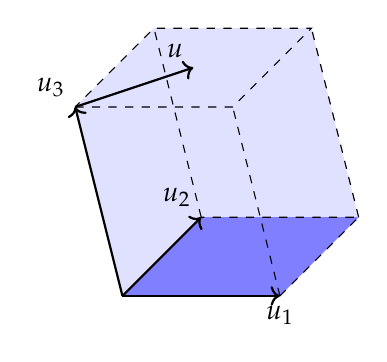
\begin{tikzpicture}[scale=2]
				\coordinate (O) at (0,0);
				\coordinate (u1) at (1,0);
				\coordinate (u2) at (0.5,0.5);
				\coordinate (u3) at (-0.3,1.2);
				\coordinate (u4) at  ($(u3) + (0.75,0.25)$);
				\coordinate (u12) at  ($(u1) + (u2)$);
				
				\fill[fill=blue, opacity=0.5]
				(O) -- (u1) -- (u12) -- (u2) -- cycle;
				
				\fill[fill=blue!40!white, opacity=0.3]
				(u2) -- (O) -- (u3) -- ($(u2)+(u3)$) -- cycle
				($(u2)+(u3)$) -- ($(u12)+(u3)$) -- (u12) -- (u2)-- cycle;
				
				\draw[thick,->] (O)-- (u1) node[below]{\( u_1 \)};
				\draw[thick,->] (O) -- (u2) node[above left]{\( u_2 \)};
				\draw[thick,->] (O) -- (u3) node[above left]{\( u_3 \)};
				\draw[thick,->] (u3) -- (u4) node[above left]{\( u \)};
				
				
				\foreach \x in {u3}{
					\draw[dashed] (\x) -- ($(\x) + (u1)$) -- ($(\x) + (u1)+ (u2)$) -- ($(\x) + (u2)$) -- cycle;}
				
				\draw[dashed] (u1) -- ($(u1) + (u2)$) -- (u2);
				
				\foreach \x in {u1,u2,u12}{
					\draw[dashed] (\x) -- ($(\x) + (u3)$);}
			\end{tikzpicture}
		\end{minipage}
		\begin{minipage}{0.3\linewidth}
			\centering
			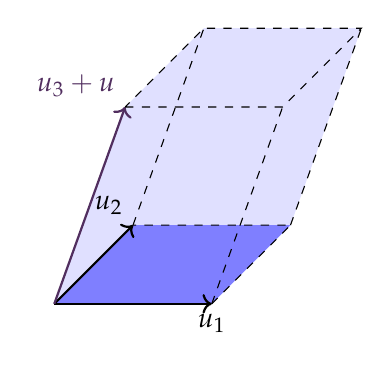
\begin{tikzpicture}[scale=2]
				\coordinate (O) at (0,0);
				\coordinate (u1) at (1,0);
				\coordinate (u2) at (0.5,0.5);
				\coordinate (u3) at (-0.3,1);
				\coordinate (u4) at  ($(u3) + (0.75,0.25)$);
				\coordinate (u12) at  ($(u1) + (u2)$);
				
				\fill[fill=blue, opacity=0.5]
				(O) -- (u1) -- (u12) -- (u2) -- cycle;
				
				\fill[fill=blue!40!white, opacity=0.3]
				(u2) -- (O) -- (u4) -- ($(u2)+(u4)$) -- cycle
				($(u2)+(u4)$) -- ($(u12)+(u4)$) -- (u12) -- (u2) -- cycle;
				
				\draw[thick,->] (O)-- (u1) node[below]{\( u_1 \)};
				\draw[thick,->] (O) -- (u2) node[above left]{\( u_2 \)};
				\draw[thick,purple,->] (O) -- (u4) node[above left]{\( u_3+u \)};
				
				\foreach \x in {u4}{
					\draw[dashed] (\x) -- ($(\x) + (u1)$) -- ($(\x) + (u1)+ (u2)$) -- ($(\x) + (u2)$) -- cycle;}
				
				\draw[dashed] (u1) -- ($(u1) + (u2)$) -- (u2);
				
				\foreach \x in {u1,u2,u12}{
					\draw[dashed] (\x) -- ($(\x) +  (u4)$);}
			\end{tikzpicture}
		\end{minipage}
		\begin{minipage}{0.3\linewidth}
			\centering
			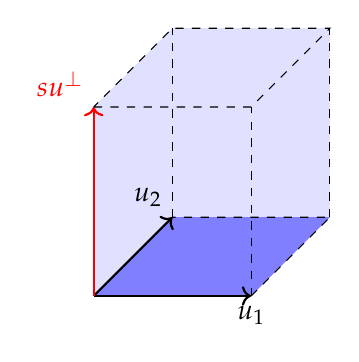
\begin{tikzpicture}[scale=2]
				\coordinate (O) at (0,0);
				\coordinate (u1) at (1,0);
				\coordinate (u2) at (0.5,0.5);
				\coordinate (u12) at ($(u1) + (u2)$);
				\coordinate (n1) at  (0,1.2);
				
				\fill[fill=blue, opacity=0.5]
				(O) -- (u1) -- (u12) -- (u2) -- cycle;
				
				\fill[fill=blue!40!white, opacity=0.3]
				(u2) -- (O) -- (n1) -- ($(u2)+(n1)$) -- cycle
				($(u2)+(n1)$) -- ($(u12)+(n1)$) -- (u12) -- (u2) -- cycle;
				
				\draw[thick,->] (O)-- (u1) node[below]{\( u_1 \)};
				\draw[thick,->] (O) -- (u2) node[above left]{\( u_2 \)};
				\draw[thick,red,->] (O) -- (n1) node[above left]{\( su^{\perp} \)};
				
				\foreach \x in {n1}{
					\draw[dashed] (\x) -- ($(\x) + (u1)$) -- ($(\x) + (u1)+ (u2)$) -- ($(\x) + (u2)$) -- cycle;}
				
				\draw[dashed] (u1) -- ($(u1) + (u2)$) -- (u2);
				
				\foreach \x in {u1,u2,u12}{
					\draw[dashed] (\x) -- ($(\x) + (n1)$);}
			\end{tikzpicture}
		\end{minipage}
		\caption{加法等式的示例 I}
		\label{cap2}
	\end{figure}
	
    补充说明一点,在一般的 \( \R^n \) 中,这样的 “垂直” 于给定 \( n-1 \) 个线性无关向量 \( u_1,\cdots,u_{n-1} \) 张成的 “平面” 的向量 \( u^{\perp} \) 也是存在的. 在欧氏空间一章我们会介绍 Gram-Schmidt 正交化方法来从已知的基出发构造之,现在只需要承认这一点. 那么这时候一定有 \( u_1,\cdots,u_{n-1},u^{\perp} \) 可以拼成 \( \F^n \) 的一组基. 因为 “垂直” 本身实际上比线性无关更强. 从一个简单的情形入手,取 \( u_1,u_2 \in \R^2, \; u_1 \perp u_2 \),考察 \( c_1u_1+c_2u_2=\bm{0} \). 那么
    
    \[ c_1u_1\T u_1+c_2 u_1\T u_2= c_1 |u_1|^2= 0 \leadsto c_1=0. \]
    
    这里 \( \alpha\T \beta \) 就是通常意义下的平面向量数量积. 另一方面,如果我们左乘 \( u_2\T \),那就能得到 \( c_2=0 \). 
	
	\vspace{2ex}
	
	\begin{figure}[htbp!] 
		\begin{minipage}{0.3\linewidth}
			\centering    
			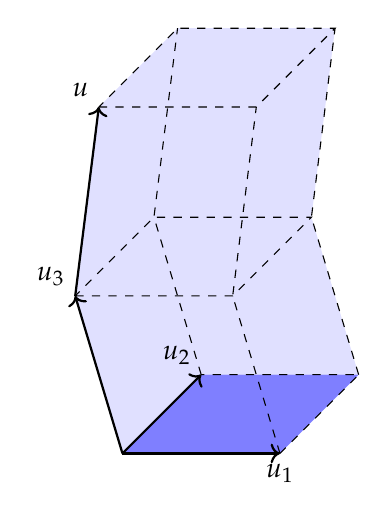
\begin{tikzpicture}[scale=2]
				\coordinate (O) at (0,0);
				\coordinate (u1) at (1,0);
				\coordinate (u2) at (0.5,0.5);
				\coordinate (u3) at (-0.3,1);
				\coordinate (u4) at  ($(u3) + (0.15,1.2)$);
				\coordinate (u12) at  ($(u1) + (u2)$);
				
				\fill[fill=blue, opacity=0.5]
				(O) -- (u1) -- (u12) -- (u2) -- cycle;
				
				\fill[fill=blue!40!white, opacity=0.3]
				(u2) -- (O) -- (u3) -- ($(u2)+(u3)$) -- cycle
				($(u2)+(u3)$) -- (u3) -- (u4) -- ($(u2)+(u4)$)-- cycle
				($(u2)+(u4)$) -- ($(u12)+(u4)$) -- ($(u12)+(u3)$) -- ($(u2)+(u3)$)-- cycle
				($(u2)+(u3)$) -- (u2) -- (u12) -- ($(u12)+(u3)$)-- cycle;
				
				\draw[thick,->] (O)-- (u1) node[below]{\( u_1 \)};
				\draw[thick,->] (O) -- (u2) node[above left]{\( u_2 \)};
				\draw[thick,->] (O) -- (u3) node[above left]{\( u_3 \)};
				\draw[thick,->] (u3) -- (u4) node[above left]{\( u \)};
				
				
				
				\foreach \x in {u3,u4}{
					\draw[dashed] (\x) -- ($(\x) + (u1)$) -- ($(\x) + (u1)+ (u2)$) -- ($(\x) + (u2)$) -- cycle;}
				
				\draw[dashed] (u1) -- ($(u1) + (u2)$) -- (u2);
				
				\foreach \x in {u1,u2,u12}{
					\draw[dashed] (\x) -- ($(\x) + (u3)$) -- ($(\x) +  (u4)$);}
			\end{tikzpicture}
		\end{minipage}
		\begin{minipage}{0.3\linewidth}
			\centering
			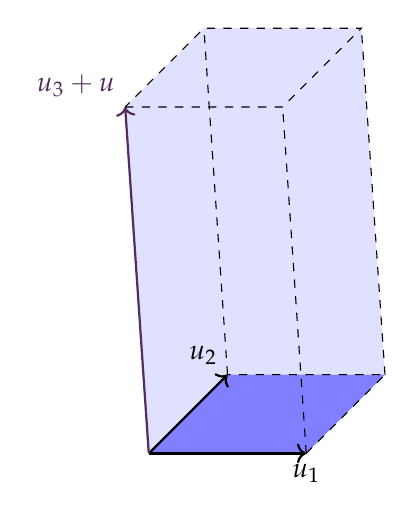
\begin{tikzpicture}[scale=2]
				\coordinate (O) at (0,0);
				\coordinate (u1) at (1,0);
				\coordinate (u2) at (0.5,0.5);
				\coordinate (u3) at (-0.3,1);
				\coordinate (u4) at  ($(u3) + (0.15,1.2)$);
				\coordinate (u12) at  ($(u1) + (u2)$);
				
				\fill[fill=blue, opacity=0.5]
				(O) -- (u1) -- (u12) -- (u2) -- cycle;
				
				\fill[fill=blue!40!white, opacity=0.3]
				(u2) -- (O) -- (u4) -- ($(u2)+(u4)$) -- cycle
				($(u2)+(u4)$) -- ($(u12)+(u4)$) -- (u12) -- (u2) -- cycle;
				
				\draw[thick,->] (O)-- (u1) node[below]{\( u_1 \)};
				\draw[thick,->] (O) -- (u2) node[above left]{\( u_2 \)};
				\draw[thick,purple,->] (O) -- (u4) node[above left]{\( u_3+u \)};
				
				\foreach \x in {u4}{
					\draw[dashed] (\x) -- ($(\x) + (u1)$) -- ($(\x) + (u1)+ (u2)$) -- ($(\x) + (u2)$) -- cycle;}
				
				\draw[dashed] (u1) -- ($(u1) + (u2)$) -- (u2);
				
				\foreach \x in {u1,u2,u12}{
					\draw[dashed] (\x) -- ($(\x) +  (u4)$);}
			\end{tikzpicture}
		\end{minipage}
		\begin{minipage}{0.3\linewidth}
			\centering
			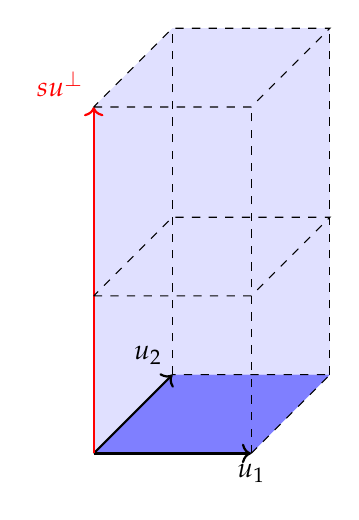
\begin{tikzpicture}[scale=2]
				\coordinate (O) at (0,0);
				\coordinate (u1) at (1,0);
				\coordinate (u2) at (0.5,0.5);
				\coordinate (u12) at ($(u1) + (u2)$);
				\coordinate (n1) at  (0,1);
				\coordinate (n2) at  (0,2.2);
				
				\fill[fill=blue, opacity=0.5]
				(O) -- (u1) -- (u12) -- (u2) -- cycle;
				
				\fill[fill=blue!40!white, opacity=0.3]
				(u2) -- (O) -- (n2) -- ($(u2)+(n2)$) -- cycle
				($(u2)+(n2)$) -- ($(u12)+(n2)$) -- (u12) -- (u2) -- cycle;
				
				\draw[thick,->] (O)-- (u1) node[below]{\( u_1 \)};
				\draw[thick,->] (O) -- (u2) node[above left]{\( u_2 \)};
				\draw[thick,red,->] (O) -- (n2) node[above left]{\( su^{\perp} \)};
				
				
				\foreach \x in {n1,n2}{
					\draw[dashed] (\x) -- ($(\x) + (u1)$) -- ($(\x) + (u1)+ (u2)$) -- ($(\x) + (u2)$) -- cycle;}
				
				\draw[dashed] (u1) -- ($(u1) + (u2)$) -- (u2);
				
				\foreach \x in {u1,u2,u12}{
					\draw[dashed] (\x) -- ($(\x) + (n1)$) -- ($(\x) +  (n2)$);}
			\end{tikzpicture}
		\end{minipage}
		\caption{加法等式的示例 II}
		\label{cap3}
	\end{figure}
	
	\vspace{2ex}
	
	(\textbf{Case II}) \ 若 \( u \) 也不能被 \( \{u_j\}_{j \neq i} \) 线性表出,给出一个分解
	\[ u_3=\lambda u^{\perp}+ \sum_{j \neq i}^{} c_ju_j, \; u=\mu u^{\perp}+ \sum_{j \neq i}^{} c_ju_j. \]
	
	一种比较幸运的情况,\( \lambda \) 和 \( \mu \) 是同号的,此时 \( u_3+u \) 在 \( u^{\perp} \) 方向的分量为 \( (\lambda+\mu) u^{\perp}=:su^{\perp} \). 那么 \( \{ u_1,u_2,u_3+tu\} \) 对 \( t \in [0,1] \) 仍为基,根据微扰不变前提,基的定向不变. 对体积而言,明显图 \ref{cap3} 的第一幅图沿着 \( u_1 \) 和 \( u_2 \) 所在平面 “平推” 就可以得到图 \ref{cap3} 的第三幅图,这个过程不改变高,也就不改变体积. 而图 \ref{cap3} 的二三幅图明显体积相同. 也就有
	
	\[ D(u_1,u_2,u_3+u)=D(u_1,u_2,u_3)+D(u_1,u_2,u). \]

	
    (\textbf{Case III}) \ 若 \( \lambda \) 和 \( \mu \) 不同号,如图 \ref{cap4} 所示. 不妨设 \( \lambda>0>\mu \) 且 \( |\lambda|>|\mu| \),那么 \( \{ u_1,u_2,u_3+tu\} \) 对 \( t \in [0,1] \) 仍为基,基的定向没有改变. 但 
    \[ D(u_1,u_2,u_3)+D(u_1,u_2,u)=V_{\lozenge(u_1,u_2,u_3)}-V_{\lozenge(u_1,u_2,u)}=V_{\lozenge(u_1,u_2,u_3+u)}=D(u_1,u_2,u_3+u), \]
    
    故结论还是成立的,若 \( \lambda+\mu=0 \),那么 \( D(u_1,u_2,u_3+u) =0 \),剩下两个有向体积刚好抵消.
	
	\vspace{2ex}
	
	\begin{figure}[htbp!]
		\begin{minipage}{0.35\linewidth}
			\centering    
			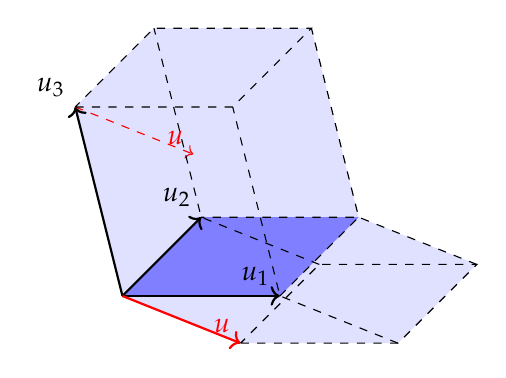
\begin{tikzpicture}[scale=2]
				\coordinate (O) at (0,0);
				\coordinate (u1) at (1,0);
				\coordinate (u2) at (0.5,0.5);
				\coordinate (u3) at (-0.3,1.2);
				\coordinate (u) at  (0.75,-0.3);
				\coordinate (u4) at  ($(u3) + (u)$);
				\coordinate (u12) at  ($(u1) + (u2)$);
				
				
				\fill[fill=blue, opacity=0.5]
				(O) -- (u1) -- (u12) -- (u2) -- cycle;
				
				\fill[fill=blue!40!white, opacity=0.3]
				(O) -- (u3) -- ($(u2)+(u3)$) -- (u2) -- cycle
				(u2)-- ($(u2)+(u3)$) -- ($(u12)+(u3)$) -- (u12) --  cycle
				(u12) -- ($(u12)+(u)$) -- ($(u1)+(u)$) -- (u1) -- cycle
				(u1) -- (O) -- (u) -- ($(u1)+(u)$) -- cycle;
				
								
				\draw[thick,->] (O)-- (u1) node[above left]{\( u_1 \)};
				\draw[thick,->] (O) -- (u2) node[above left]{\( u_2 \)};
				\draw[thick,->] (O) -- (u3) node[above left]{\( u_3 \)};
				\draw[dashed,red,->] (u3) -- (u4) node[above left]{\( u \)};
				\draw[thick,red,->] (O) -- (0.75,-0.3) node[above left]{\( u \)};
				
				
				\foreach \x in {u3,u}{
					\draw[dashed] (\x) -- ($(\x) + (u1)$) -- ($(\x) + (u1)+ (u2)$) -- ($(\x) + (u2)$) -- cycle;}
				
				\draw[dashed] (u1) -- ($(u1) + (u2)$) -- (u2);
				
				\foreach \x in {u1,u2,u12}{
					\draw[dashed] ($(\x) +  (u)$) -- (\x) -- ($(\x) + (u3)$);}
			\end{tikzpicture}
		\end{minipage}
		\begin{minipage}{0.25\linewidth}
			\centering
			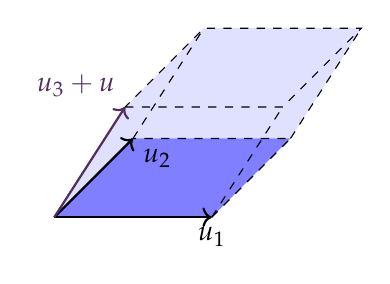
\begin{tikzpicture}[scale=2]
				\coordinate (O) at (0,0);
				\coordinate (u1) at (1,0);
				\coordinate (u2) at (0.5,0.5);
				\coordinate (u3) at (-0.3,1);
				\coordinate (u4) at  ($(u3) + (0.75,-0.3)$);
				\coordinate (u12) at  ($(u1) + (u2)$);
				
				\fill[fill=blue, opacity=0.5]
				(O) -- (u1) -- (u12) -- (u2) -- cycle;
				
				\fill[fill=blue!40!white, opacity=0.3]
				(u2) -- (O) -- (u4) -- ($(u2)+(u4)$) -- cycle
				($(u2)+(u4)$) -- ($(u12)+(u4)$) -- (u12) -- (u2) -- cycle;
				
				\draw[thick,->] (O)-- (u1) node[below]{\( u_1 \)};
				\draw[thick,->] (O) -- (u2) node[below right]{\( u_2 \)};
				\draw[thick,purple,->] (O) -- (u4) node[above left]{\( u_3+u \)};
				
				\foreach \x in {u4}{
					\draw[dashed] (\x) -- ($(\x) + (u1)$) -- ($(\x) + (u1)+ (u2)$) -- ($(\x) + (u2)$) -- cycle;}
				
				\draw[dashed] (u1) -- ($(u1) + (u2)$) -- (u2);
				
				\foreach \x in {u1,u2,u12}{
					\draw[dashed] (\x) -- ($(\x) +  (u4)$);}
			\end{tikzpicture}
		\end{minipage}
		\begin{minipage}{0.25\linewidth}
			\centering
			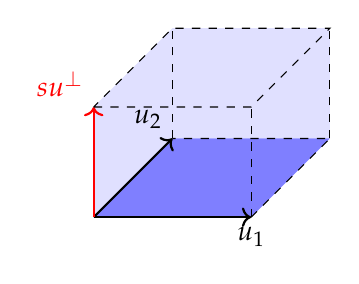
\begin{tikzpicture}[scale=2]
				\coordinate (O) at (0,0);
				\coordinate (u1) at (1,0);
				\coordinate (u2) at (0.5,0.5);
				\coordinate (u12) at ($(u1) + (u2)$);
				\coordinate (n1) at  (0,0.7);
				
				\fill[fill=blue, opacity=0.5]
				(O) -- (u1) -- (u12) -- (u2) -- cycle;
				
				\fill[fill=blue!40!white, opacity=0.3]
				(u2) -- (O) -- (n1) -- ($(u2)+(n1)$) -- cycle
				($(u2)+(n1)$) -- ($(u12)+(n1)$) -- (u12) -- (u2) -- cycle;
				
				\draw[thick,->] (O)-- (u1) node[below]{\( u_1 \)};
				\draw[thick,->] (O) -- (u2) node[above left]{\( u_2 \)};
				\draw[thick,red,->] (O) -- (n1) node[above left]{\( su^{\perp} \)};
				
				\foreach \x in {n1}{
					\draw[dashed] (\x) -- ($(\x) + (u1)$) -- ($(\x) + (u1)+ (u2)$) -- ($(\x) + (u2)$) -- cycle;}
				
				\draw[dashed] (u1) -- ($(u1) + (u2)$) -- (u2);
				
				\foreach \x in {u1,u2,u12}{
					\draw[dashed] (\x) -- ($(\x) + (n1)$);}
			\end{tikzpicture}
		\end{minipage}
		
		\caption{加法等式的示例 III}
		\label{cap4}
	\end{figure}
	
	\vspace{2ex}
	
	虽然最后一个结论的几何诠释分类显得有些复杂,本质上没有什么内容. 读者如果愿意用行列式来理解可以跳过. 总之,我们从 \( \R^3 \) 中得到了上述原材料,看似不劳而获. 我们马上会发现,这三条性质几乎完全刻画了 \( D \),最多差一个比例常数.
	
\end{enumerate}

上面的三条性质,尽管从源头上来说需要一些度量的刻画,但性质描述本身没有对域 \( \F \) 有多少限制,于是我们自然想推广到一般的域 \( \F \) 上. 称满足上述三条性质的函数为 \( \F^n \) 上的交错形式.
 
\begin{definition}[交错形式] \label{2.3.23}
	设 \( n \in \mathbb{Z}_{\geq 1}\),给出 \( D: \F^n \to \F \) 满足
	\begin{enumerate}[(i)]
		\item \textbf{线性} \ 设 \( 1 \leq i \leq n \),以及 \( u_i,u \in \F^n \) 和 \( c \in \F \),有
		\[ D(u_1,\cdots,u_i+u,\cdots,u_n)=D(u_1,\cdots,u_i,\cdots,u_n)+D(u_1,\cdots,u,\cdots,u_n). \]
		\[ D(u_1,\cdots,cu_i,\cdots,u_n)=cD(u_1,\cdots,u_i,\cdots,u_n). \]
		
		\item 若存在 \( 1 \leq i<j \leq n \) 使得 \( u_i=u_j \),有
		\[ D(u_1,\cdots,u_i,\cdots,u_j,\cdots,u_n)=0. \]
	\end{enumerate}
	
    那么称 \( D \) 为 \( \F \) 上的一个 \( n \) 元交错形式,并记所有这样的映射构成集合 \( \mathcal{D}_{\F^n} \). 特别规定 \( \mathcal{D}_{\F^0}=\F \). 上述 (ii) 的规定对 \( n=1 \) 是多余的.
\end{definition}

\begin{remark} \label{2.3.24}
	有的教材上对于第二点规定的是 \textbf{交错性}: 交换变元 \(u_i \) 和 \( u_j \) 的顺序导致变号. 即
	\[  D(u_1,\cdots,u_i,\cdots,u_j,\cdots,u_n)=- D(u_1,\cdots,u_j,\cdots,u_i,\cdots,u_n). \]
	
	但在一般 \( \tz F=2 \) 的域中,未必有 \( 2x=0 \Rightarrow x=0 \). 而定义 \ref{2.3.23} (2) 其实蕴含了上述交错性. \textbf{提示: }考虑
	\[ D(u_1,\cdots,u_i+u_j,\cdots,u_i+u_j,\cdots,u_n)=0, \]
	
	然后用定义 \ref{2.3.23} (1) 依次对第 \( i \) 和第 \( j \) 个变元线性展开.
\end{remark}

那么 \( \R^3 \) 上的行列式,或者说有向体积,就是一种 \( 3 \) 元交错形式. 为了从定义 \ref{2.3.23} 中得到更多性质,我们引入逆序数的概念.

\begin{definition}[逆序数] \label{2.3.25}
	设正整数 \( i_1,\cdots,i_m \) 两两不同,考察集合
	\[ \text{Inv}(i_1,\cdots,i_m):=\{(p,q) \in \mathbb{Z}^2 \mid 1 \leq p<q \leq m, i_p>i_q \}. \]
	
	称 \( \text{Inv}(i_1,\cdots,i_m) \) 中的元素个数 \( |\text{Inv}(i_1,\cdots,i_m)|:= \sigma(i_1,\cdots,i_m) \) 为这个排列的逆序数. 若 \( \sigma(i_1,\cdots,i_m) \) 为奇数,那么称排列 \( (i_1,\cdots,i_m) \) 为奇排列,否则为偶排列.
\end{definition}

\begin{example} \label{2.3.26}
	给定正整数 \( (i_1,\cdots,i_n) \) 为 \( (1,\cdots,n) \) 的一个排列,那么 
	\[ \sigma(i_1,\cdots,i_n)=(n-i_n)+\sigma(i_1,\cdots,i_{n-1}). \]
\end{example}

\begin{proof}
	只需要注意到,从 \( \text{Inv}(i_1,\cdots,i_n) \) 到 \( \text{Inv}(i_1,\cdots,i_{n-1}) \),集合中只减少了类似 \( (p,n) \ (1 \leq p \leq n-1) \) 这样的元素. 下面统计这种类型的元素个数. 由于 \( \{ i_1,\cdots,i_{n-1} \}= \{1,2,\cdots,n\} \textbackslash \{i_n\} \). 也就是 \( i_1,\cdots,i_{n-1} \) 中比 \( i_n \) 大的数只有 \( i_n+1,\cdots,n \) 共 \( n-i_n \) 个,用定义 \ref{2.3.25} 得到欲证等式.
\end{proof}

\begin{proposition} \label{2.3.27}
	给定正整数 \( (i_1,\cdots,i_n) \) 为 \( (1,\cdots,n) \) 的一个排列,且 \( \sigma(i_1,\cdots,i_n)=k \),那么对排列 \( (i_1,\cdots,i_n) \) 可以经过 \( k \) 次元素之间的对换使得其变为 \( (1,\cdots,n) \). 
\end{proposition}

\begin{proof}
	若 \( k=0 \),那么命题已经成立. 否则,必定存在 \( 1 \leq p \leq n-1 \) 使得 \( i_{p+1}<i_{p} \). 这时对调 \( i_p \) 和 \( i_{p+1} \),也就是
	
	\[ (\cdots,i_p,i_{p+1},\cdots) \ (\text{I}) \leadsto (\cdots,i_{p+1},i_{p},\cdots) \ (\text{II}). \]
	
	\( i_p \) 和 \( i_{p+1} \) 不参与构成的数对,在 (I) 中和在 (II) 中是否逆序是一样的; \( i_p \) 或 \( i_{p+1} \) 和其他数构成的数对,在 (I) 中和在 (II) 中是否逆序也是一样的. 只有 \( i_p \) 和 \( i_{p+1} \) 之间,它在 (I) 中是逆序,在 (II) 中就是顺序. 也就是对调后排列的逆序数变为 \( k-1 \). 若 \( k-1 \geq 1 \),可以继续找到相邻两数逆序,仿照上述操作继续进行. 当逆序数为 0 时,排列必定形如  \( (1,\cdots,n) \).
\end{proof}
 
\begin{proposition} \label{2.3.28}
	给定正整数 \( (i_1,\cdots,i_n) \) 为 \( (1,\cdots,n) \) 的一个排列,记其逆序数为 \( \sigma_1 \). 现将其中的两个元素 \( i_p \) 和 \( i_q \ (1 \leq p<q \leq n) \) 对换,所得新排列 \( (i_1,\cdots,i_{p-1},i_q,i_{p+1},\cdots,i_{q-1},i_p,i_{q+1},\cdots,i_n) \) 的逆序数记为 \( \sigma_2 \). 那么 \( \sigma_1 \) 和 \( \sigma_2 \) 的奇偶性不同,换言之,
	\[ (-1)^{\sigma_1}+(-1)^{\sigma_2}=1. \]
\end{proposition}

\begin{proof}
	先考虑相邻两个数 \( i_p \) 和 \( i_{p+1} \) 对换的情形. 
	\[ (\cdots,i_p,i_{p+1},\cdots) \ (\text{I}) \leadsto (\cdots,i_{p+1},i_{p},\cdots) \ (\text{II}). \]
	
	 \( i_p \) 和 \( i_{p+1} \) 不参与构成的数对,在 (I) 中和在 (II) 中是否逆序是一样的; \( i_p \) 或 \( i_{p+1} \) 和其他数构成的数对,在 (I) 中和在 (II) 中是否逆序是一样的,只有 \( i_p \) 和 \( i_{p+1} \) 之间,它在 (I) 中是顺序,那么它在 (II) 中就是逆序,反之,在 (I) 中是逆序,在 (II) 中就是顺序. 也就是相邻两个数对调后,逆序数必定加一或者减一. 进而,奇偶性改变. 
	 
	 现在考虑任意两个数 \( i_p \) 和 \( i_q \) 对换,这一点可以通过 \( i_p \) 先依次和 \( i_{p+1}, i_{p+2},\cdots,i_{q-1}, i_q \) 互换,然后 \( i_q \) 再和 \( i_{p+1}, i_{p+2},\cdots,i_{q-1} \) 互换,累计 \( 2(q-p)-1 \) 次相邻两个数的互换实现,这是奇数次改变排列奇偶性的互换,必然使得逆序数奇偶性改变.
\end{proof}

\begin{practice}
	给定正整数 \( (i_1,\cdots,i_n) \) 为 \( (1,\cdots,n) \) 的一个排列,记其逆序数为 \( \sigma_1 \). 设 \( (i_1,\cdots,i_n) \) 经过 \( s \) 次元素对换变回 \( (1,2,\cdots,n) \). 证明: \( s \equiv \sigma_1 \pmod 2 \).
\end{practice}

\begin{proof}
	用命题 \ref{2.3.28} 考察排列的奇偶性.
\end{proof}

\begin{lemma} \label{2.3.29}
	给定正整数 \( (i_1,\cdots,i_n) \) 为 \( (1,\cdots,n) \) 的一个排列,且 \( D \in \mathcal{D}_{\F^n} \),那么
	\[ D(u_{i_1},\cdots,u_{i_n})=(-1)^{\sigma(i_1,\cdots,i_n)} D(u_1,\cdots,u_n). \]
\end{lemma}

\begin{proof}
	利用注 \ref{2.3.24},交错形式具有交错性,也就是每次两个向量之间的对换都会改变符号,再利用命题 \ref{2.3.27},存在一个 \( \sigma(i_1,\cdots,i_n) \) 次两个元素对换组成的操作,使得 \( u_{i_1},\cdots,u_{i_n} \) 变为 \( u_1,\cdots,u_n \). 即证.
\end{proof}

\begin{theorem} \label{2.3.30}
	取定 \( \F^n \) 的一组有序基 \( (\bme_1,\cdots,\bme_n) \),任取向量 \( u_1,\cdots,u_n \in \F^n \),那么由定义 \ref{2.3.14},存在唯一 \( A=(a_{ij}) \in \F\n \) 使得 \( (u_1,\cdots,u_n)=(\bme_1,\cdots,\bme_n)A \). 那么对任意 \( D \in \mathcal{D}_{\F^n} \) 都必须有
	\begin{equation}
		 D(u_1,\cdots,u_n)= \sum_{(i_1,\cdots,i_n)}^{} (-1)^{\sigma(i_1,\cdots,i_n)} \ a_{i_1,1}a_{i_2,2}\cdots a_{i_n,n} \ D(\bme_1,\cdots,\bme_n),
		 \label{equ2.3.1}
	\end{equation}
	
	这表示对 \( (1,2,\cdots,n) \) 的所有排列求和. 换言之,这说明为了确定 \( D \) 的映射效果,只需要观察 \( D \) 在选定的一组基 \( \bme_1,\cdots,\bme_n \) 上的取值即可.
\end{theorem}

\begin{proof}
	由于
	\[ u_j=\sum_{i=1}^{n} a_{ij}\bme_i, \; 1 \leq j \leq n. \]
	
	利用定义 \ref{2.3.23} (1) 有
	\begin{align*}
		D(u_1,\cdots,u_n) &= \sum_{i_1=1}^{n} a_{i_1,1} \ D(\bme_{i_1},u_2,\cdots,u_n), \\
		&= \sum_{i_1=1}^{n} \sum_{i_2=1}^{n}\cdots \sum_{i_n=1}^{n} a_{i_1,1}a_{i_2,2}\cdots a_{i_n,n} \ D(\bme_{i_1},\bme_{i_2},\cdots,\bme_{i_n}).
	\end{align*}
	
	上述求和除去存在 \( \bme_{i_p}=\bme_{i_q} \) 交错形式取值为 0 的项,一共有 \( n! \) 项,且刚好遍历 \( (1,2,\cdots,n) \) 的所有排列. 另一方面,再利用引理 \ref{2.3.29},就有
	\[ D(u_1,\cdots,u_n)= \sum_{(i_1,\cdots,i_n)}^{} (-1)^{\sigma(i_1,\cdots,i_n)} \ a_{i_1,1}a_{i_2,2}\cdots a_{i_n,n} \ D(\bme_1,\cdots,\bme_n). \]
\end{proof}

\begin{proposition} \label{2.3.31}
	在定理 \ref{2.3.30} 的条件下,式 (\ref{equ2.3.1}) 等价于
	\[ D(u_1,\cdots,u_n)= \sum_{(j_1,\cdots,j_n)}^{} (-1)^{\sigma(j_1,\cdots,j_n)} \ a_{1,j_1}a_{2,j_2}\cdots a_{n,j_n} \ D(\bme_1,\cdots,\bme_n). \]
\end{proposition}

\begin{proof}
	我们不妨考虑一个一般的情形,设 \( a_{i_1,1}a_{i_2,2}\cdots a_{i_n,n} \) 经过 \( s \) 次元素的对换变成 \( a_{k_1,j_1}a_{k_2,j_2}\cdots a_{k_n,j_n} \). 这就蕴含了 \( (i_1,\cdots,i_n) \) 经过 \( s \) 次对换变成 \( (k_1,\cdots,k_n) \) 以及 \( (1,\cdots,n) \) 经过 \( s \) 次对换变成 \( (j_1,\cdots,j_n) \). 那么由命题 \ref{2.3.28} 有
	\[ (-1)^{\sigma(k_1,\cdots,k_n)}=(-1)^{s+\sigma(i_1,\cdots,i_n)}, \; (-1)^{\sigma(j_1,\cdots,j_n)}=(-1)^s.\] 
	
	也就是
	\[ (-1)^{2s+\sigma(i_1,\cdots,i_n)}=(-1)^{\sigma(i_1,\cdots,i_n)}=(-1)^{\sigma(k_1,\cdots,k_n)+\sigma(j_1,\cdots,j_n)}. \]
	
	再用命题 \ref{2.3.27},知道 \( (i_1,\cdots,i_n) \) 可以通过若干次对换变回 \( (1,\cdots,n) \). 那么取 \( (k_1,\cdots,k_n)=(1,\cdots,n) \). 这时,式 (\ref{equ2.3.1}) 中的每一项就可以写为
	\[ (-1)^{\sigma(i_1,\cdots,i_n)} \ a_{i_1,1}a_{i_2,2}\cdots a_{i_n,n} =(-1)^{\sigma(j_1,\cdots,j_n)+0} \ a_{1,j_1}a_{2,j_2}\cdots a_{n,j_n}. \]
	
	这时候注意到,原先求和的时候 \( (i_1,\cdots,i_n) \) 是遍历全排列的,也就是 \( a_{i_1,1}a_{i_2,2}\cdots a_{i_n,n} \) 是互不相同的项,那么经过若干次对调后,对元素本身不变,也就是还是互不相同的项,一共 \( n! \) 项. 那么 \( (j_1,\cdots,j_n) \) 也应当遍历 \( (1,2,\cdots,n) \) 的全排列,于是求和可以改写为
	\[ D(u_1,\cdots,u_n)= \sum_{(j_1,\cdots,j_n)}^{} (-1)^{\sigma(j_1,\cdots,j_n)} \ a_{1,j_1}a_{2,j_2}\cdots a_{n,j_n} \ D(\bme_1,\cdots,\bme_n). \]
	
	上述过程明显可逆,也就是上述两式等价.
\end{proof}

定理 \ref{2.3.30} 给出了 \( n \) 元交错形式的一种刻画,如果 \( D \) 存在,那么必定要满足定理 \ref{2.3.30} 或者命题 \ref{2.3.31} 给出的等式,相当于一种必要条件. 但这时候 \( D \) 是否存在还未可知,下面的定理 \ref{2.3.32} 刻画了 \( n \) 元交错形式的存在性.

\begin{theorem} \label{2.3.32}
	取定 \( \F^n \) 的一组有序基 \( (\bme_1,\cdots,\bme_n) \),那么存在唯一 \( D_{\bm{e}} \in \mathcal{D}_{\F^n} \) 使得 \( D(\bme_1,\cdots,\bme_n)=1 \).
\end{theorem}

\begin{proof}
	任取向量 \( u_1,\cdots,u_n \in \F^n \),那么由定义 \ref{2.3.14},存在唯一 \( A=(a_{ij}) \in \F\n \) 使得 \( (u_1,\cdots,u_n)=(\bme_1,\cdots,\bme_n)A \). 这时候取
	\[ D_{\bm{e}}(u_1,\cdots,u_n):=\sum_{(i_1,\cdots,i_n)}^{} (-1)^{\sigma(i_1,\cdots,i_n)} \ a_{i_1,1}a_{i_2,2}\cdots a_{i_n,n}. \]
	
	接下来自然问这么定义会满足我们对 \( n \) 元交错形式,也就是定义 \ref{2.3.23} 的要求吗? (i) 线性是很容易的,无非就是其中有一项要拆成两项,或者是其中一项发生了数量乘法,当然可以提出求和号外. 具体细节留给读者. 我们只验证 (ii). 这时候要求 \( n \geq 2 \). 若 \( u_p=u_q \),那么 \( a_{i,p}=a_{i,q} \) 对任意 \( 1 \leq i \leq n \) 都成立. 接下来,我们用 \( S_{n-2} \) 表示 \( i_1,\cdots,i_{p-1},i_{p+1},\cdots,i_{q-1},i_{q+1},\cdots,i_n \) 这 \( n-2 \) 个元素取值在 \( \{1,2,\cdots,n\} \) 的所有排列,共 \( A_{n}^{n-2}=n!/2 \) 个. 留意
	\[ a_{i_1,1}\cdots {\color{red}a_{i_p,p}} \cdots {\color{green!40!black} a_{i_q,q}} \cdots a_{i_n,n}= a_{i_1,1}\cdots {\color{green!40!black}a_{i_q,p}} \cdots { \color{red} a_{i_p,q}} \cdots a_{i_n,n}. \]
	
	用命题 \ref{2.3.28} 就有
	\begin{align*}
		\sum_{(i_1,\cdots,i_n)}^{} (-1)^{\sigma(i_1,\cdots,i_n)} \ a_{i_1,1}a_{i_2,2}\cdots a_{i_n,n} &=\sum_{S_{n-2}}^{} [(-1)^{\sigma(i_1,\cdots,i_q,\cdots,i_p,\cdots,i_n)}+ (-1)^{\sigma(i_1,\cdots,i_p,\cdots,i_q,\cdots,i_n)}] a_{i_1,1}a_{i_2,2}\cdots a_{i_n,n}, \\
		&=\sum_{S_{n-2}}^{} 0 \cdot a_{i_1,1}a_{i_2,2}\cdots a_{i_n,n}=0. 
	\end{align*}
	
	至此,我们确定了 \(D_{\bm{e}} \in \mathcal{D}_{\F^n} \). 另一方面, \( D_{\bm{e}}(\bme_1,\cdots,\bme_n) \) 的展开式中 \( a_{i_1,1} \) 非零当且仅当 \( i_1=1 \),且此时 \( a_{1,1}=1 \),后续同理,那么非零项只有
	\[ D_{\bm{e}}(\bme_1,\cdots,\bme_n)=(-1)^{\sigma(1,2,\cdots,n)} a_{11}\cdots a_{nn}=1. \]
	
	至于唯一性,利用命题 \ref{2.3.31},一个交错形式完全由其在 \( \bme_1,\cdots,\bme_n \) 上的取值唯一确定.
\end{proof}

一个很自然的疑问? 我们在定理 \ref{2.3.32} 中给出的构造 \( D_{\bm{e}} \) 和先前谈论的有向体积有什么联系呢? 在 \( n \) 维情况定义的交错形式和行列式存在什么关系呢? 下面的定理告诉我们,在相差一个 \( \F \) 中常数的情况下,有向体积就等同于我们定义的 \( D_{\bm{e}} \). 而行列式的观察留待后面小节讨论.

\begin{theorem} \label{2.3.33}
	设 \( D \in \mathcal{D}_{\F^n} \),那么存在唯一 \( c \in \F \),使得 \( D=cD_{\bme} \),其中 \( D_{\bme} \) 如同定理 \ref{2.3.32} 所构造. 换言之,其实有 \( \dim \mathcal{D}_{\F^n}=1 \).
\end{theorem}

\begin{proof}
	利用命题 \ref{2.3.31},一个交错形式完全由其在 \( \bme_1,\cdots,\bme_n \) 上的取值唯一确定,而 \( D_{\bm{e}}(\bme_1,\cdots,\bme_n)=1 \),那么取 \( c=D(\bme_1,\cdots,\bme_n) \),就有 \( D=cD_{\bm{e}} \). 换言之,就是 \( \mathcal{D}_{\F^n} \) 中的元素全部线性相关,且 \( D_{\bm{e}} \) 可以充当一个基. 
	
	当然了,我们还没有定义 \( \mathcal{D}_{\F^n} \) 上的线性结构,这是很容易定义的. 对 \( D_1,D_2 \in \mathcal{D}_{\F^n} \) 以及 \( c \in \F \),定义
	\[ (D_1+cD_2)(u_1,\cdots,u_n)=D_1(u_1,\cdots,u_n)+c \cdot [D_2(u_1,\cdots,u_n)]. \]
\end{proof}

\subsubsection{行列式的映射定义与组合展开式}

下面我们给出行列式的第二种定义,请读者先默认我们还未定义过行列式,下面是你第一次见到这个名词. 我们马上就会证明两种定义的等价性.

\begin{definition}[行列式的映射定义] \label{2.3.34}
	设 \( A \in \F\n \ (n \in \mathbb{Z}_{\geq 1}) \),线性变换 \( \varphi_{A}: \F^n \to \F^n, \; X \mapsto AX \) 诱导出 \( \varphi^*_{A}: \mathcal{D}_{\F^n} \to \mathcal{D}_{\F^n}, \; D \mapsto D^* \). 这里 \( D^* \) 的定义为
	\[ D^*(v_1,\cdots,v_n)=D(Av_1,\cdots,Av_n), \; \forall \; D \in \mathcal{D}_{\F^n}, \; v_1,\cdots,v_n \in \F^n. \]
	
	容易验证这时候 \( D^* \in \mathcal{D}_{\F^n} \). 由定理 \ref{2.3.33},那么存在唯一常数 \( c \in F \),使得 \( D^*=cD \). 定义 \( c=\det A \),表示矩阵 \( A \) 的行列式. 对 \( n=0 \),我们定义 \( \det A=1 \).
\end{definition}

如果将 \( D \) 和 \( D^* \) 想象为有向体积,那么行列式无非就是 \( \varphi_{A} \) 带来的体积伸缩量,从 \( D(v_1,\cdots,v_n) \) 到 \( D(Av_1,\cdots,Av_n) \). 这一点将在多元重积分的换元公式中自然而然的出现,因为对满足逆映射定理的可微向量值函数,局部存在可逆线性映射 \( Jf: X \mapsto JX \),其中 \( J \) 为 \( f \) 的 Jacobi 矩阵. 那么局部体积的改变量的绝对值就是 \( |\det J| \),作为一个比例系数存在.

当 \( A \) 可逆时,由于 \( AX=O \) 仅有零解,那么 \( c_1Av_1+\cdots+c_nAv_n= \bm{0}= A(c_1v_1+\cdots+c_nv_n) \Rightarrow c_1v_1+\cdots+c_nv_n=\bm{0} \). 那么 \( \varphi_{A} \) 保持线性关系. 如果取 \( v_1,\cdots,v_n \) 为一组基,那么体积必定不为零,且 \( Av_1,\cdots,Av_n \) 也为一组基,体积也不为零,体积伸缩量 \( \det A \) 当然也不为零,符合我们在命题 \ref{2.2.13} 中的刻画. 


另一方面,若 \( A \) 不可逆,那么 \( AX=O \) 存在非零解,不妨记为 \( X=\beta \neq \bm{0} \),如果 \( v_1,\cdots,v_n \) 为一组基,那么存在唯一的 \( c_1,\cdots,c_n \in \F \) 使得 \( \beta=c_1v_1+\cdots+c_nv_n \),且由于 \( \beta \neq \bm{0} \),故 \( c_1,\cdots,c_n \) 当然不会全为零,此时用 \( A \) 左乘,就有
\[ c_1(Av_1)+\cdots+c_n(Av_n)=A\beta=\bm{0}. \]

也就说明 \( Av_1,\cdots,Av_n \) 线性相关,那么有向体积自然为零. 说明 \( \varphi_{A} \) 带来的伸缩量就是直接打到零了,即 \( \det A=0 \),完美符合命题 \ref{2.2.14}. 这只是一种初步验证,我们接下来给出定义 \ref{2.3.34} 的具体表达式.

\begin{definition}[行列式的组合展开式定义] \label{2.3.35}
	在定义 \ref{2.3.34} 的基础上,设 \( A=(a_{ij}) \),那么
	\[ \det A= \sum_{(i_1,\cdots,i_n)}^{} (-1)^{\sigma(i_1,\cdots,i_n)} \ a_{i_1,1}a_{i_2,2}\cdots a_{i_n,n}. \]
	
	用命题 \ref{2.3.31},那么还可以写为
	\[ \det A= \sum_{(j_1,\cdots,j_n)}^{} (-1)^{\sigma(j_1,\cdots,j_n)} \ a_{1,j_1}a_{2,j_2}\cdots a_{n,j_n}. \]
	
	这其实说明了 \( \det A=\det A\T \). 符合性质 \ref{2.2.2}. 
\end{definition}

\begin{proof}
	取定 \( \F^n \) 的一组基 \( e_1,\cdots,e_n \). 接下来注意到 \( (A\bme_1,\cdots,A\bme_n)=(\bme_1,\cdots,\bme_n)A \) 即可. 那么由定理 \ref{2.3.30},
	\[ D^*(\bme_1,\cdots,\bme_n)=\sum_{(i_1,\cdots,i_n)}^{} (-1)^{\sigma(i_1,\cdots,i_n)} \ a_{i_1,1}a_{i_2,2}\cdots a_{i_n,n} \ D(\bme_1,\cdots,\bme_n)=(\det A) D(\bme_1,\cdots,\bme_n). \]
	
	对 \( D = \mathcal{O} \) 上式永远成立,只考虑 \( D \neq \mathcal{O} \),那么 \( D(\bme_1,\cdots,\bme_n) \neq 0 \),因为基下的取值唯一决定了 \( D \). 两边消去 \( D(\bme_1,\cdots,\bme_n) \) 即可. 另一方面,如果给出定义 \ref{2.3.35},将上述证明倒着写回去,又能得到 \( D^*=(\det A) D \),回到定义 \ref{2.3.34}. 也就是这两个定义本身是等价的.
\end{proof}

\subsubsection{定义的等价性}

我们只需要验证定义 \ref{2.2.1} 和定义 \ref{2.3.35} 等价,因为定义 \ref{2.3.35} 和定义 \ref{2.3.34} 已经等价.

\begin{theorem}
	定义 \ref{2.2.1} \( \Leftrightarrow \) 定义 \ref{2.3.35}.
\end{theorem}

\begin{proof}
	首先定义 \ref{2.2.1} 等价于行列式可按第 \( n \) 行展开. 前者蕴含后者是推论 \ref{2.2.5} 的结果,而如果想从行列式可按第 \( n \) 行展开推出行列式可以按第一列展开,你可以类似性质 \ref{2.2.2} 的证明思路,先证明交换行列式的两行行列式改变符号,然后验证行列式可以按任意行展开,最后证明转置不改变行列式的值. 在此不多赘述.
	
	若行列式可以按第 \( n \) 行展开,下面用归纳法证明定义 \ref{2.3.35}. 当 \( n=1 \) 时显然成立,假设命题对 \( n-1 \) 阶行列式成立,研究 \( n \) 阶行列式,那么
	\[ \det A= \sum_{j=1}^{n} (-1)^{n+j} a_{nj} M_{nj}= \sum_{j=1}^{n} (-1)^{2j} (-1)^{n-j} a_{nj} M_{nj}= \sum_{j=1}^{n}  (-1)^{n-j} a_{nj} M_{nj}. \]
	
	其中 
	\[ a_{nj}M_{nj}= \sum_{(k_1,\cdots,k_{n-1}) }^{} (-1)^{\sigma(k_1,\cdots,k_{n-1})} a_{1,k_1}\cdots a_{n-1,k_{n-1}} a_{nj}. \]
	
	其中 \( k_1,\cdots,k_{n-1} \) 为 \( \{1,2,\cdots,n\}-\{j\} \) 的一个全排列. 那么由例 \ref{2.3.26} 知道
	\begin{align*}
		\det A &= \sum_{j=1}^{n} \sum_{(k_1,\cdots,k_{n-1}) }^{}  (-1)^{(n-j)+\sigma(k_1,\cdots,k_{n-1})} a_{1,k_1}\cdots a_{n-1,k_{n-1}} a_{nj}, \\
		&= \sum_{j=1}^{n} \sum_{(k_1,\cdots,k_{n-1}) }^{}  (-1)^{\sigma(k_1,\cdots,k_{n-1},j)} a_{1,k_1}\cdots a_{n-1,k_{n-1}}a_{nj}, \\
		&= \sum_{(k_1,\cdots,k_{n-1},k_n) }^{}  (-1)^{\sigma(k_1,\cdots,k_{n-1},k_n)} a_{1,k_1}\cdots a_{n-1,k_{n-1}}a_{n,k_n}.
	\end{align*}
    
    这恰好是 \( n! \) 个不同乘积的求和,那么必定遍及全排列,即证. 将上述过程反之,就证明了等价性.
    
\end{proof}

\begin{practice}
	设 \( S_n \) 为 \( (1,2,\cdots,n) \) 所有全排列构成的集合,证明其中奇偶排列各半.
\end{practice}

\begin{proof}
	一种方法是用定义 \ref{2.3.35},考虑元素全为 1 的行列式. 还可以考虑,记 \( A_n \subseteq S_n \) 为所有偶排列构成的集合,\( B_n \subseteq S_n \) 为所有奇排列构成的集合. 令 \( f:A_n \to B_n, (i_1,\cdots,i_n) \mapsto (1,2)(i_1,\cdots,i_n) \). 其中 \( (1,2) \) 表示对调排列中的 1 和 2. 那么 \( f^2=\mathrm{id} \). 容易验证 \( f \) 为单射. 再任取 \( (j_1,\cdots,j_n) \) 为奇排列,有 \( f[f(j_1,\cdots,j_n)]=(j_1,\cdots,j_n) \). 说明 \( f \) 为满射. 故 \( |A_n|=|B_n| \).
\end{proof}


\subsubsection{一些计算实例 II}

定义 \ref{2.3.35} 一般不用来计算具体行列式,因为一共需要处理 \( n! \) 项,计算比较繁琐,如果我们使用初等变换打洞,量级只有 \( n^3 \). 它在某些定性判断上很有优势. 例如,如果我们要处理一个整数矩阵,希望判断它是否可逆. 取 \( \varphi: \mathbb{Z} \to \mathbb{Z}_n, \; k \mapsto [k] \),其中 \( n \) 为某个整数. 容易验证这是一个环同态,即保持数的加法和乘法,
\[ [k_1]+[k_2]=[k_1+k_2], \; [k_1][k_2]=[k_1k_2], \]

这一点在 \S 1 已经验证过. 那么 
\[ \varphi(\det A)= \det [A], \; A=([a_{ij}]). \]

这纯粹是因为定义 \ref{2.3.35} 中只涉及到数的加法和乘法,那么 \( \varphi \) 完全保持运算. 如果说 \( \det [A] \neq 0 \),那么 \( \det A \notin n\mathbb{Z}:=\{nk \mid k \in \mathbb{Z} \} \),也就更不可能为零了,反之如果 \( \det A \neq 0 \),却未必有 \( \det [A] \neq 0 \). 我们有时候验证 \( \det [A] \neq 0 \) 这一更强的条件,就可以简化问题的讨论.


\begin{example} \label{2.3.37}
	证明: \[
	\begin{vmatrix}
		1 & 2 & \cdots & 2^{2020} & 2^{2021} \\
		2 & 1 & \cdots & 2^{2019} & 2^{2020} \\
		\vdots & \vdots & \ddots & \vdots & \vdots \\
		2^{2020} & 2^{2019} & \cdots & 1 & 2 \\
		2^{2021} & 2^{2020} & \cdots & 2 & 1
	\end{vmatrix} \neq 0.
	\]
\end{example}

\begin{solution}
	将所有元素 \( \text{mod} \ 2 \),也就是构造环同态 \( \varphi: \mathbb{Z} \to \mathbb{Z}_2, \; k \mapsto [k] \),得到
	\[ \det [A]=\begin{vmatrix}
		1 & 0 & \cdots & 0 & 0 \\
		0 & 1 & \cdots & 0 & 0 \\
		\vdots & \vdots & \ddots & \vdots & \vdots \\
		0 & 0 & \cdots & 1 & 0 \\
		0 & 0 & \cdots & 0 & 1
	\end{vmatrix}=1.  \]
	
	那么 \( \det A \neq 0 \).
\end{solution}

\begin{example}
	设 \( A  \) 是 \( 2024 \) 阶方阵,主对角线上全是偶数,其余的都是奇数. 证明该矩阵可逆.
\end{example}

\begin{solution}
	和例 \ref{2.3.37} 完全相同.
\end{solution}

\begin{example}
	证明: 当 \( n \) 为奇数时有 \[
	\begin{vmatrix}
		1 & 2 & 3 & \cdots & n-1 & n \\
		2^2 & 3^2 & 4^2 & \cdots & n^2 & (n+1)^2 \\
		3^3 & 4^3 & 5^3 & \cdots & (n+1)^3 & (n+1)^3 \\
		\vdots & \vdots & \vdots & \ddots & \vdots & \vdots \\
		n^n & (n+1)^n & (n+1)^n & \cdots & (n+1)^n & (n+1)^n
	\end{vmatrix} \neq 0.
	\]
\end{example}

\begin{solution}
	将所有元素 \( \text{mod} \ 2 \),也就是构造环同态 \( \varphi: \mathbb{Z} \to \mathbb{Z}_2, \; k \mapsto [k] \),得到
	\[ \det [A]=\begin{vmatrix}
		* & * & \cdots & * & 1 \\
		* & * & \cdots & 1 & 0 \\
		\vdots & \vdots & \ddots & \vdots & \vdots \\
		* & 1 & \cdots & 0 & 0 \\
		1 & 0 & \cdots & 0 & 0
	\end{vmatrix}.  \]
	
	那么 \( \det [A] \) 的展开式中非零项只有斜对角线下来的乘积,即
	\[ \det [A]= (-1)^{\sigma(n,n-1,\cdots,1)} a_{1n}a_{2,n-1}\cdots a_{n,1}=(-1)^{\sigma(n,n-1,\cdots,1)}=1^{\sigma(n,n-1,\cdots,1)}=1 \neq 0. \]
	
	这里只需要注意到 \( -1=1 \) 在 \( \mathbb{Z}_2 \) 中.
\end{solution}

\begin{example}
	设 \( A = (a_{ij}) \in \mathbb{R}^{2025 \times 2025} \),满足
	\[
	a_{ii} = i^3 + 3i^2 + 2i, \quad
	a_{ij} = \left\{ \begin{array}{lr}
	3(i - j) + 1, & i < j, \\
	3(i + j) + 2, & i > j,
	\end{array}\right.
	\]
	
	证明: \( 3 \mid \det A \).
\end{example}

\begin{solution}
	将所有元素 \( \text{mod} \ 3 \),也就是构造环同态 \( \varphi: \mathbb{Z} \to \mathbb{Z}_3, \; k \mapsto [k] \),得到
	\[ \det [A]=\begin{vmatrix}
		* & 1 & \cdots & 1 & 1 \\
		-1 & * & \cdots & 1 & 1 \\
		\vdots & \vdots & \ddots & \vdots & \vdots \\
		-1 & -1 & \cdots & * & 1 \\
		-1 & -1 & \cdots & -1 & *
	\end{vmatrix}.  \]
	
	这是一个奇数阶反对称行列式,那么 \( \det [A]=\det (-[A]\T)= -\det [A]\T= -\det [A] \). 在 \( \mathbb{Z}_3 \) 中 \( 2\det [A]=0 \) 蕴含 \( \det [A]=0 \). 回到 \( \mathbb{Z} \) 中就是 \( 3 \mid \det A \).
\end{solution}



\subsection{间奏: 行列式的其他性质}

到这里为止,我们本节的所有任务几乎都已经完成了,得到了可逆矩阵的判定定理,\( A \) 为方阵时 \( AX=\beta \) 的公式解,解释了行列式这一工具的几何意义和有向体积的关联. 为了知识的完整性,下面再介绍两个有关行列式计算的定理,它们偶尔会使用到. 证明只是擘画大概思路,不拘泥于具体的细节.

\subsubsection{Laplace 展开定理}

Laplace 展开定理指的是按多行或者多列展开行列式,计算量上相比按一行或一列展开几乎不变,偶尔遇到含零比较多的行列式用这点或许更快. 理论上的意义肯定是大于实际操作的意义的.

有了 Laplace 展开定理后,计算引理 \ref{2.2.8} 和命题 \ref{2.2.25} 对应的分块矩阵行列式就有了全新的方法,具体可以参考课本上的证明,没有很大难度. 下面先介绍子式,主子式和顺序主子式的概念,这三者在后续会偶尔碰到,不妨现在一并全部认识一下,Laplace 展开定义只用到子式的概念. 

\begin{definition}[\( k \) 阶子式,余子式,代数余子式]
	取定 \( n \) 阶行列式 \( \det A \) 中第 \( i_1 \) 行, 第 \( i_2 \) 行,\( \cdots \), 第 \( i_k \) 行以及第 \( j_1 \) 列, 第 \( j_2 \) 列,\( \cdots \), 第 \( j_k \) 列交点上的元素,其中
	\[
	1 \leq i_1 < i_2 < \cdots < i_k \leq n, \quad 1 \leq j_1 < j_2 < \cdots < j_k \leq n,
	\]
	按原来在 \( A \) 中的位置构成一个 \( k \) 阶行列式,称为 \( A \) 的一个 \( k \) 阶子式,记为
	\begin{equation}
		A\begin{bmatrix}
			i_1 & i_2 & \cdots & i_k \\
			j_1 & j_2 & \cdots & j_k
		\end{bmatrix}
		= \begin{vmatrix}
			a_{i_1 j_1} & a_{i_1 j_2} & \cdots & a_{i_1 j_k} \\
			a_{i_2 j_1} & a_{i_2 j_2} & \cdots & a_{i_2 j_k} \\
			\vdots & \vdots & \ddots & \vdots \\
			a_{i_k j_1} & a_{i_k j_2} & \cdots & a_{i_k j_k}
		\end{vmatrix}. 
		\label{equ2.4.1}
	\end{equation}

	在 \( \det A \) 中去掉第 \( i_1 \), \( i_2 \),\( \cdots \),\( i_k \) 行以及第 \( j_1 \), \( j_2 \),\( \cdots \),\( j_k \) 列后的元素,按原来相对位置构成一个 \( (n-k) \) 阶行列式,称为式 (\ref{equ2.4.1}) 的余子式,记为
	\[
	M\begin{bmatrix}
		i_1 & i_2 & \cdots & i_k \\
		j_1 & j_2 & \cdots & j_k
	\end{bmatrix}
	\]
	
	令
	\[
	p = i_1 + i_2 + \cdots + i_k, \quad
	q = j_1 + j_2 + \cdots + j_k,
	\]
	
	记
	\[
	\hat{A}\begin{bmatrix}
		i_1 & i_2 & \cdots & i_k \\
		j_1 & j_2 & \cdots & j_k
	\end{bmatrix}
	= (-1)^{p + q} M\begin{bmatrix}
		i_1 & i_2 & \cdots & i_k \\
		j_1 & j_2 & \cdots & j_k
	\end{bmatrix}
	\]
	称为式 (\ref{equ2.4.1}) 的代数余子式.
	
\end{definition}


\begin{definition}[主子式和顺序主子式]
	设 \( A \) 是 \( n \) 阶方阵,\( A \) 的 \( k \) 阶子式
	\[
	A\begin{bmatrix}
		i_1 & i_2 & \cdots & i_k \\
		i_1 & i_2 & \cdots & i_k
	\end{bmatrix}
	= \begin{vmatrix}
		a_{i_1 i_1} & a_{i_1 i_2} & \cdots & a_{i_1 i_k} \\
		a_{i_2 i_1} & a_{i_2 i_2} & \cdots & a_{i_2 i_k} \\
		\vdots & \vdots & \ddots & \vdots \\
		a_{i_k i_1} & a_{i_k i_2} & \cdots & a_{i_k i_k}
	\end{vmatrix}
	\]
	称为 \( A \) 的一个 \( k \) 阶主子式. 特别取 \( (i_1,\cdots,i_k)=(1,\cdots,k) \),称为 \( A \) 的 \( k \) 阶顺序主子式.
\end{definition}

\begin{theorem}[Laplace 展开定理] \label{2.4.3}
	设 \( A \) 是 \( n \) 阶方阵,在 \( A \) 中任取 \( k \) 行或列,那么选自这 \( k \) 行或列的全部 \( k \) 阶子式与它们对应的代数余子式的乘积之和等于 \( \det A \). 即若取定
	\[
	1 \leq i_1 < i_2 < \cdots < i_k \leq n,
	\]
	
	则
	\begin{equation}
		\det A = \sum_{1 \leq j_1 < j_2 < \cdots < j_k \leq n}
		A\begin{bmatrix}
			i_1 & i_2 & \cdots & i_k \\
			j_1 & j_2 & \cdots & j_k
		\end{bmatrix}
		\hat{A}\begin{bmatrix}
			i_1 & i_2 & \cdots & i_k \\
			j_1 & j_2 & \cdots & j_k
		\end{bmatrix}.
		\label{equ2.4.2}
	\end{equation}

	同样,若取定 \( k \) 列 \( 1 \leq j_1 < j_2 < \cdots < j_k \leq n \),则
	\begin{equation}
		\det A = \sum_{1 \leq i_1 < i_2 < \cdots < i_k \leq n}
		A\begin{bmatrix}
			i_1 & i_2 & \cdots & i_k \\
			j_1 & j_2 & \cdots & j_k
		\end{bmatrix}
		\hat{A}\begin{bmatrix}
			i_1 & i_2 & \cdots & i_k \\
			j_1 & j_2 & \cdots & j_k
		\end{bmatrix}.
		\label{equ2.4.3}
	\end{equation}
\end{theorem}

\begin{proof}
	我们只证明式 (\ref{equ2.4.2}),式 (\ref{equ2.4.3}) 可以由 \( \det A\T= \det A \) 得到. 注意到式 (\ref{equ2.4.2}) 右端的展开式中有 \( C_n^k k! (n-k)!=n! \) 项,且都互不相同. 只需要证明这 \( n! \) 项都是 \( \det A \) 展开式 (定义 \ref{2.3.35}) 中的项且符号一致即可.
	
	为了简化讨论,我们先把第 \( i_1,\cdots,i_k \) 行经过对换调整到第 \( 1 \sim k \) 行,而剩余的行调整到 \( (k+1) \sim n \) 行后仍维持原先顺序. 计算这样需要对换的次数. 首先让 \( i_1 \) 对换到第 \( 1 \) 行,且不改变后续行的顺序,需要让第 \( i_1 \) 行先后和 \( i_1-1,\cdots,2,1 \) 行对换,需要 \( i_1-1 \) 次. 类似地,第 \( i_2 \) 行需要对调到第 \( 2 \) 行,且不改变后续行的顺序,\( \cdots \). 行的对调需要 \( (i_1-1)+\cdots+(i_k-k)=p-k(k+1)/2 \) 次. 列的对调就需要 \( q-k(k+1)/2 \) 次. 得到一共需要对调的次数就是 \( (p+q)-k(k+1) \) 次,这与 \( p+q \) 同奇偶.
	
	经过上述操作后得到的矩阵记为 \( \hat{A}=(\hat{a}_{ij}) \),那么 \( \det A= (-1)^{p+q} \det \hat{A} \). 且原先矩阵中每一个子式对应的子矩阵 \( A_1 \) 和余子式对应的子矩阵 \( A_2 \) 都跑到了下面分块矩阵的 \( B \) 和 \( C \) 位置,
	\[ \bordermatrix{
		& k & n-k \cr
		k & B & * \cr
		n-k & * & C
	} \]
	
	且 \( \det B=\det A_1, \; \det C=\det A_2 \). 又因为 \( \det B \) 在 \( \det \hat{A} \) 中的代数余子式为 \( \det C \). 那么 \( \det B \det C \) 中的每一项都形如
	\[ (-1)^{\sigma(i_1,\cdots,i_k)}\hat{a}_{1,i_1}\cdots \hat{a}_{1,i_k} \cdot (-1)^{\sigma(i_{k+1},\cdots,i_n)} \hat{a}_{k+1,i_{k+1}}\cdots \hat{a}_{n,i_n},  \]
	
	其中 \( (i_1,\cdots,i_k) \) 为 \( (1,\cdots,k) \) 的全排列,而 \( (i_{k+1},\cdots,i_n) \) 为 \( (k+1,\cdots,n) \) 的全排列,那么 \( \sigma(i_1,\cdots,i_n)=\sigma(i_1,\cdots,i_k)+\sigma(i_{k+1},\cdots,i_n) \). 也就说明 \( \det B \det C  \) 中的每一项都是 \( \det \hat{A} \) 的项,且符号相同. 那么
	\[ (-1)^{p+q}\det B \det C=\det A_1 [(-1)^{p+q} \det A_2] \] 
	中的每一项都是 \( \det A \) 的项,且符号相同. 而这正是 \( \det A \) 的一个 \( k \) 阶子式和其代数余子式的乘积.
\end{proof}

\begin{example}
	计算下列 \( 2n \) 阶行列式:
	\[
	D_n=\begin{vmatrix}
		a &        &        &        &  & b \\
		& \ddots &        &  & \iddots &   \\
		&        & a      & b   &     &   \\
		&  & b      & a   &     &   \\
		& \iddots&      &   & \ddots     &   \\
		b &        &        &       & & a
	\end{vmatrix}_{(2n \times 2n)}
	\]
\end{example}

\begin{solution}
	用定理 \ref{2.4.3},即 Laplace 展开,按第 \( 1, 2n \) 行展开,那么只有
	\[ A\begin{bmatrix}
		1 & 2n \\
		1 & 2n
	\end{bmatrix} \]
	
	这一二阶主子式非零,那么 \( D_n=(-1)^{2(2n+1)}(a^2-b^2)D_{n-1}=(a^2-b^2)D_{n-1}=(a^2-b^2)^n \).
\end{solution}

\subsubsection{Cauchy\(-\)Binet 公式}

Cauchy\(-\)Binet 公式是对命题 \ref{2.2.9} 在非方阵情形的推广.

\begin{theorem}[Cauchy\(-\)Binet] \label{2.4.5}
	设 \( A \) 是 \( m \times n \) 矩阵,\( B \) 是 \( n \times m \) 矩阵,则
	\[
	\det(AB) =
	\left\{
	\begin{array}{lr}
		0, & n < m, \\
		\det A \cdot \det B, & n = m, \\
		\displaystyle
		\sum_{1 \leq i_1 < i_2 < \cdots < i_m \leq n}
		\det\left(
		A\begin{bmatrix}
			1 & 2 & \cdots & m \\
			i_1 & i_2 & \cdots & i_m
		\end{bmatrix}
		\right)
		\cdot
		\det\left(
		B\begin{bmatrix}
			i_1 & i_2 & \cdots & i_m \\
			1 & 2 & \cdots & m
		\end{bmatrix}
		\right), & n > m.
	\end{array}
	\right.
	\]
\end{theorem}

\begin{proof}
	回忆我们在命题 \ref{2.2.9} 所操作的,无非就是如下的分块初等变换
	\[ \begin{bmatrix}
		E_n & O \\
		-A & E_m
	\end{bmatrix} \Omega:=\begin{bmatrix}
	E_n & O \\
	-A & E_m
	\end{bmatrix}\begin{bmatrix}
		E_n & B \\
		A & O
	\end{bmatrix}=\begin{bmatrix}
	E_n & B \\
	O & -AB 
	\end{bmatrix}.
	\]
	
	用命题 \ref{2.2.25} 和引理 \ref{2.2.8},两边同时取行列式得到 \( \det(AB)=(-1)^m \det \Omega \). 当 \( n<m \) 时,对 \( \Omega \) 按第 \( (n+1) \sim (n+m) \) 行展开,那么不可能存在非零子式,也就是 \( \det \Omega=0 \). \( n=m \) 就是命题 \ref{2.2.9}. 对 \( n>m \) 的情形,对 \( \det \Omega \) 还是按第 \( (n+1) \sim (n+m) \) 行展开,记
	\[ \hat{A}\begin{bmatrix}
		1 & 2 & \cdots & m \\
		i_1 & i_2 & \cdots & i_m
	\end{bmatrix}=:(-1)^{nm+(1+\cdots+m)+(i_1+\cdots+i_m)} \det C. \]
	
	为
	\[ A\begin{bmatrix}
		1 & 2 & \cdots & m \\
		i_1 & i_2 & \cdots & i_m
	\end{bmatrix} \]
	
	在 \( \det \Omega \) 中的代数余子式. 其中 \( 1 \leq i_1 < i_2 < \cdots < i_m \leq n \). 设 \( \{j_1,\cdots,j_{n-m} \}=\{1,\cdots,n\}-\{i_1,\cdots,i_m\} \),且 \( j_1<\cdots<j_{n-m} \). 那么
	\[ \det C= \det (\varepsilon_{j_1},\cdots,\varepsilon_{j_{n-m}},B). \]
	
	对其再按第 \( 1 \sim (n-m) \) 列展开,只有子式 
	\[ C\begin{bmatrix}
		j_1 & j_2 & \cdots & j_{n-m} \\
		1 & 2 & \cdots & {n-m}
	\end{bmatrix} \]
	
	非零,且其在 \( \det C \) 中的代数余子式为
	\[ (-1)^{(j_1+\cdots+j_{n-m})+(1+\cdots+n-m)}B\begin{bmatrix}
		i_1 & i_2 & \cdots & i_m \\
		1 & 2 & \cdots & m
	\end{bmatrix}. \]
	
	下面验算 \( (-1) \) 的总幂次,即
	\begin{align*}
		&\quad nm+(1+\cdots+m)+(i_1+\cdots+i_m)+(j_1+\cdots+j_{n-m})+(1+\cdots+n-m) \\
		&=nm+\frac{n(n+1)+m(m+1)+(n-m)(n-m+1)}{2} \\
		&=n(n+1)+m^2.
	\end{align*}
    
    那么
    \[ \det \Omega= (-1)^{m^2} \sum_{1 \leq i_1 < i_2 < \cdots < i_m \leq n}
    \det\left(
    A\begin{bmatrix}
    	1 & 2 & \cdots & m \\
    	i_1 & i_2 & \cdots & i_m
    \end{bmatrix}
    \right)
    \cdot
    \det\left(
    B\begin{bmatrix}
    	i_1 & i_2 & \cdots & i_m \\
    	1 & 2 & \cdots & m
    \end{bmatrix}
    \right). \]
    
    回到 \( \det (AB)=(-1)^m \det \Omega \) 代入即证.
\end{proof}

\begin{corollary} \label{2.4.6}
   设 \( A \) 是 \( m \times n \) 矩阵,\( B \) 是 \( n \times s \) 矩阵,令 \( C = AB \),则 \( C \) 的任一 \( r \; (\leq \min\{m,s\})\) 阶子式为
	\[
	C\begin{bmatrix}
		i_1 & i_2 & \cdots & i_r \\
		j_1 & j_2 & \cdots & j_r
	\end{bmatrix}
	=
	\left\{
	\begin{array}{lr}
		0, & n < r, \\
		\displaystyle \sum_{1 \le l_1 < \cdots < l_r \le n}
		A\begin{bmatrix}
			i_1 & i_2 & \cdots & i_r \\
			l_1 & l_2 & \cdots & l_r
		\end{bmatrix}
		B\begin{bmatrix}
			l_1 & l_2 & \cdots & l_r \\
			j_1 & j_2 & \cdots & j_r
		\end{bmatrix}, & n \ge r.
	\end{array}
	\right.
	\]
\end{corollary}

\begin{proof}
	只需要注意到
	\[ C\begin{bmatrix}
		i_1 & i_2 & \cdots & i_r \\
		j_1 & j_2 & \cdots & j_r
	\end{bmatrix}=\det \left( \begin{bmatrix}
	a_{i_1 1} & a_{i_1 2} & \cdots & a_{i_1 n} \\
	a_{i_2 1} & a_{i_2 2} & \cdots & a_{i_2 n} \\
	\vdots    & \vdots    &        & \vdots    \\
	a_{i_r 1} & a_{i_r 2} & \cdots & a_{i_r n}
	\end{bmatrix} \begin{bmatrix}
	b_{1 j_1} & b_{1 j_2} & \cdots & b_{1 j_r} \\
	b_{2 j_1} & b_{2 j_2} & \cdots & b_{2 j_r} \\
	\vdots    & \vdots    &        & \vdots    \\
	b_{n j_1} & b_{n j_2} & \cdots & b_{n j_r}
	\end{bmatrix} \right). \]
	
	然后用定理 \ref{2.4.5} 即可.
\end{proof}

\begin{remark}
	定理 \ref{2.4.5} 中 \( n<m \) 以及推论 \ref{2.4.6} 中 \( n<r \) 的部分可以利用 \textit{\S 5 向量组的线性关系和极大线性无关组} 该节的一个秩不等式 \( r(AB) \leq \min\{ r(A),r(B) \} \leq n \) 配合秩的子式定义来说明.
\end{remark}

\begin{proposition}
	设 \( A \in \R\mn \),证明 \( AA\T \) 的任意主子式非负.
\end{proposition}

\begin{proof}
	用推论 \ref{2.4.6},当 \( r \leq n \) 时
	\[ AA\T
	\begin{bmatrix}
		i_1 & i_2 & \cdots & i_r \\
		i_1 & i_2 & \cdots & i_r
	\end{bmatrix}
	=
	\sum_{1 \leq j_1 < j_2 < \cdots < j_r \leq n}
	\left( A
	\begin{bmatrix}
		i_1 & i_2 & \cdots & i_r \\
		j_1 & j_2 & \cdots & j_r
	\end{bmatrix}
	\right)^2
	\geq 0. \]
	
	当 \(  r>n \) 时,主子式的值为零,也是非负的.
\end{proof}

\subsection{尾声: 再谈可逆矩阵}

在本节的最后,我们回到可逆矩阵,探究与之相关的一些问题,并且给出一种适合用于计算的求逆方法. 在先前的讨论中,我们得到的 \( A^{-1}= 1/(\det A) A^* \) 用来求解逆矩阵的方法,计算量实在太大了,是 \( n^2 \cdot (n-1)!=n \cdot n! \) 量级. 这对高阶矩阵几乎无法计算.

\subsubsection{初等变换求逆}

在前面我们已经知道 Guass-Jordan 消元法可以将一个可逆矩阵仅通过初等行变换变为它的简化行阶梯形矩阵 \( E_n \),也就是对给定 \( A \in \gf \),存在 \(  P \in \gf \),使得 \( PA=E_n \leadsto A^{-1}=P \). 考虑如下的初等行变换
\[ (A,E_n) \leadsto P(A,E_n)=(E_n,P)=(E_n,A^{-1}). \]

让问题又回到了先前关于  Guass-Jordan 消元法这一算法的讨论. 这个算法的操作复杂度仅有 \( n^3 \),效率大大提升. 命题 \ref{2.2.13} 同时还说明了一个可逆矩阵也可以仅通过初等列变换变为它的简化行阶梯形矩阵 \( E_n \). 存在 \( Q \in \gf \),使得 \( AQ=E_n \leadsto A^{-1}=Q \). 下面的初等列变换也是可行的,
\[ \begin{pmatrix}
	A \\ E_n
\end{pmatrix} \leadsto \begin{pmatrix}
A \\ E_n
\end{pmatrix}Q=\begin{pmatrix}
E_n \\ Q
\end{pmatrix}=\begin{pmatrix}
E_n \\ A^{-1}
\end{pmatrix}. \]

这种方法还可以推广到解线性方程组和矩阵方程上. 设 \( A \in \gf, \; B \in \F\nm \),那么矩阵方程 \( AX=B \) 有唯一解 \( X=A^{-1}B \). 对应到如下的初等行变换
\[ (A,B) \leadsto P(A,B)=(E_n,PB)=(E_n,A^{-1}B). \]

特别取 \( m=1 \),那么矩阵方程就变成我们在定理 \ref{2.2.15} 所讨论的线性方程组,显然这种方法比起 Cramer 法则更有实用性. 如果矩阵方程的形式变为 \( XA=B \leadsto X=BA^{-1} \),就对应初等列变换 
\[ \begin{pmatrix}
	A \\ B
\end{pmatrix} \leadsto \begin{pmatrix}
A \\ B
\end{pmatrix}Q=\begin{pmatrix}
	E_n \\ BQ
\end{pmatrix}=\begin{pmatrix}
	E_n \\ BA^{-1}
\end{pmatrix}. \]

结合上述两种方法,就可以求解方程 \( AXB=C, \; A,B \in \gf \). 下面看一个复杂一些的例子.

\begin{example}
	求循环矩阵 \( A \) 的逆矩阵 \( A^{-1} \):
	\[
	A = 
	\begin{pmatrix}
		1 & 2 & 3 & \cdots & n-1 & n \\
		n & 1 & 2 & \cdots & n-2 & n-1 \\
		n-1 & n & 1 & \cdots & n-3 & n-2 \\
		\vdots & \vdots & \vdots & \ddots & \vdots & \vdots \\
		2 & 3 & 4 & \cdots & n & 1
	\end{pmatrix}.
	\]
		
\end{example}

\begin{solution}
	对 \( (A,E_n) \) 实行初等变换
	\setcounter{MaxMatrixCols}{12}
	\[ 	\begin{pNiceMatrix}
		1 & 2 & 3 & \cdots & n-1 & n & \Vdots[line-style=standard]  & 1 & 0 & 0 & \cdots & 0 \\
		n & 1 & 2 & \cdots & n-2 & n-1 & & 0 & 1 & 0 & \cdots & 0 \\
		n-1 & n & 1 & \cdots & n-3 & n-2 & & 0 & 0 & 1 & \cdots & 0 \\
		\vdots & \vdots & \vdots & \ddots & \vdots & \vdots & & \vdots & \vdots & \vdots & \ddots & \vdots  \\
		2 & 3 & 4 & \cdots & n & 1 & \Vdots[line-style={dashed}] & 0 & 0 & 0 & \cdots & 1
	\end{pNiceMatrix} \]
	
	\vspace{2ex}
	
	先将第 \( 2 \sim n \) 行都加到第一行,并同时除以 \( s:=n(n+1)/2 \),得到
	\[ 	\begin{pNiceMatrix}
		1 & 1 & 1 & \cdots & 1 & 1 & \Vdots[line-style=standard]  & 1/s & 1/s & 1/s & \cdots & 1/s \\
		n & 1 & 2 & \cdots & n-2 & n-1 & & 0 & 1 & 0 & \cdots & 0 \\
		n-1 & n & 1 & \cdots & n-3 & n-2 & & 0 & 0 & 1 & \cdots & 0 \\
		\vdots & \vdots & \vdots & \ddots & \vdots & \vdots & & \vdots & \vdots & \vdots & \ddots & \vdots  \\
		2 & 3 & 4 & \cdots & n & 1 & \Vdots[line-style={dashed}] & 0 & 0 & 0 & \cdots & 1
	\end{pNiceMatrix} \]
	
	\vspace{2ex}
	
	从第 \( 2 \) 行起,每一行减去其下一行得到
	
	\[ 	\begin{pNiceMatrix}
		1 & 1 & 1 & \cdots & 1 & 1 & \Vdots[line-style=standard]  & 1/s & 1/s & 1/s & \cdots & 1/s \\
		1 & 1-n & 1 & \cdots & 1 & 1 & & 0 & 1 & -1 & \cdots & 0 \\
		1 & 1 & 1-n & \cdots & 1 & 1 & & 0 & 0 & 1 & \cdots & 0 \\
		\vdots & \vdots & \vdots & \ddots & \vdots & \vdots & & \vdots & \vdots & \vdots & \ddots & \vdots  \\
		2 & 3 & 4 & \cdots & n & 1 & \Vdots[line-style={dashed}] & 0 & 0 & 0 & \cdots & 1
	\end{pNiceMatrix} \]
	
	\vspace{2ex}
	
	消去第一列除第一行外的所有元素
	
	\[ 	\begin{pNiceMatrix}
		1 & 1 & 1 & \cdots & 1 & 1 & \Vdots[line-style=standard]  & 1/s & 1/s & 1/s & \cdots & 1/s \\
		0 & -n & 0 & \cdots & 0 & 0 & & -1/s & 1-1/s & -1-1/s & \cdots & -1/s \\
		0 & 0 & -n & \cdots & 0 & 0& & -1/s & -1/s & 1-1/s & \cdots & -1/s \\
		\vdots& \vdots & \vdots & \ddots & \vdots & \vdots & & \vdots & \vdots & \vdots & \ddots & \vdots  \\
		0 & 1 & 2 & \cdots & n-2 & -1 & \Vdots[line-style={dashed}] & -2/s & -2/s & -2/s & \cdots & 1-2/s
	\end{pNiceMatrix} \]
	
	\vspace{2ex}
	
	先将右端矩阵提取一个 \( 1/s \) 
	
	\[ 	\begin{pNiceMatrix}
		1 & 1 & 1 & \cdots & 1 & 1 & \Vdots[line-style=standard]  & 1 & 1 & 1 & \cdots & 1 \\
		0 & -n & 0 & \cdots & 0 & 0 & & -1 & s-1 & -s-1 & \cdots & -1 \\
		0 & 0 & -n & \cdots & 0 & 0& & -1 & -1 & s-1 & \cdots & -1 \\
		\vdots& \vdots & \vdots & \ddots & \vdots & \vdots & & \vdots & \vdots & \vdots & \ddots & \vdots  \\
		0 & 1 & 2 & \cdots & n-2 & -1 & \Vdots[line-style={dashed}] & -2 & -2 & -2 & \cdots & s-2
	\end{pNiceMatrix} \]
	
	\vspace{2ex}
	
	第 \( 2 \sim (n-1) \) 行同时除以 \( -1/n \)
	
	\[ 	\begin{pNiceMatrix}
		1 & 1 & 1 & \cdots & 1 & 1 & \Vdots[line-style=standard]  & 1 & 1 & 1 & \cdots & 1 \\
		0 & 1 & 0 & \cdots & 0 & 0 & & 1/n & (1-s)/n & (s+1)/n & \cdots & 1/n \\
		0 & 0 & 1 & \cdots & 0 & 0& & 1/n & 1/n & (1-s)/n & \cdots & 1/n \\
		\vdots& \vdots & \vdots & \ddots & \vdots & \vdots & & \vdots & \vdots & \vdots & \ddots & \vdots  \\
		0 & 1 & 2 & \cdots & n-2 & -1 & \Vdots[line-style={dashed}] & -2 & -2 & -2 & \cdots & s-2
	\end{pNiceMatrix} \]
	
	\vspace{2ex}
	
	第 \( 1 \) 行减去第 \( 2 \sim (n-1) \) 行
	
	\[ 	\begin{pNiceMatrix}
		1 & 0 & 0 & \cdots & 0 & 1 & \Vdots[line-style=standard]  & 2/n & (2+s)/n & 2/n & \cdots & (2-s)/n \\
		0 & 1 & 0 & \cdots & 0 & 0 & & 1/n & (1-s)/n & (s+1)/n & \cdots & 1/n \\
		0 & 0 & 1 & \cdots & 0 & 0& & 1/n & 1/n & (1-s)/n & \cdots & 1/n \\
		\vdots& \vdots & \vdots & \ddots & \vdots & \vdots & & \vdots & \vdots & \vdots & \ddots & \vdots  \\
		0 & 1 & 2 & \cdots & n-2 & -1 & \Vdots[line-style={dashed}] & -2 & -2 & -2 & \cdots & s-2
	\end{pNiceMatrix} \]
	
	\vspace{2ex}
	
	用第 \( 2 \sim (n-1) \) 行将第 \( n \) 行除最后一列外全打为零,这需要一点计算,对右侧矩阵的 \( (n,1) \) 元,实际上变为
	\[ -2-\sum_{i=1}^{n-2} \frac{i}{n}= -\frac{2n+(n-1)(n-2)/2}{n}=-\frac{n^2+n+2}{2n}=-\frac{s+1}{n}. \]
	
	再计算右侧矩阵的 \( (n,2) \) 元
	\[ -2-\sum_{i=1}^{n-2} \frac{i}{n}+2\frac{s}{n}=-\frac{s+1}{n}+\frac{s}{n}=-\frac{1}{n}. \]
	
	
	\( (n,j) \ (3 \leq j \leq n-1) \) 元
	\[ -2-\sum_{i=1}^{n-2} \frac{i}{n}-(j-1)\frac{s}{n}+j\frac{s}{n}=-\frac{s+1}{n}+\frac{s}{n}=-\frac{1}{n}. \]
	
	以及 \( (n,n) \) 元
	\[ s-2-\sum_{i=1}^{n-2} \frac{i}{n}-\frac{(n-2)s}{n}=s-\frac{s+1}{n}-\frac{(n-2)s}{n}=\frac{s-1}{n}. \]
	
	\[ 	\begin{pNiceMatrix}
		1 & 0 & 0 & \cdots & 0 & 1 & \Vdots[line-style=standard]  & 2/n & (2+s)/n & 2/n & \cdots & (2-s)/n \\
		0 & 1 & 0 & \cdots & 0 & 0 & & 1/n & (1-s)/n & (s+1)/n & \cdots & 1/n \\
		0 & 0 & 1 & \cdots & 0 & 0& & 1/n & 1/n & (1-s)/n & \cdots & 1/n \\
		\vdots& \vdots & \vdots & \ddots & \vdots & \vdots & & \vdots & \vdots & \vdots & \ddots & \vdots  \\
		0 & 0 & 0 & \cdots & 0 & -1 & \Vdots[line-style={dashed}] & -(s+1)/n & -1/n & -1/n & \cdots & (s-1)/n
	\end{pNiceMatrix} \]
	
	\vspace{2ex}
	
	最后一行加到第一行
	
	\[ 	\begin{pNiceMatrix}
		1 & 0 & 0 & \cdots & 0 & 0 & \Vdots[line-style=standard]  & (1-s)/n & (1+s)/n & 1/n & \cdots & 1/n \\
		0 & 1 & 0 & \cdots & 0 & 0 & & 1/n & (1-s)/n & (s+1)/n & \cdots & 1/n \\
		0 & 0 & 1 & \cdots & 0 & 0& & 1/n & 1/n & (1-s)/n & \cdots & 1/n \\
		\vdots& \vdots & \vdots & \ddots & \vdots & \vdots & & \vdots & \vdots & \vdots & \ddots & \vdots  \\
		0 & 0 & 0 & \cdots & 0 & -1 & \Vdots[line-style={dashed}] & -(s+1)/n & -1/n & -1/n & \cdots & (s-1)/n
	\end{pNiceMatrix} \]
	
	\vspace{2ex}
	
	最后将最后一行乘以 \( (-1) \),并把先前提取的 \( 1/s \) 乘回去,得到所求逆矩阵
	\[ A^{-1}= \frac{1}{ns} \begin{pmatrix}
		1-s & 1+s & 1 & \cdots & 1 \\
		1 & 1-s & 1+s & \cdots & 1 \\
		1 & 1 & 1-s & \cdots & 1 \\
		\vdots& \vdots & \vdots & \ddots & \vdots \\
		1+s & 1 & 1 & \cdots & 1-s 
	\end{pmatrix}. \]
\end{solution}

\subsubsection{抽象型求逆问题}

一类在这个部分常碰到的判断逆矩阵的问题,往往是给出一个多项式 \( f(\lambda) \in \F[\lambda]\) 零化矩阵 \( A \),即 \( f(A)=O \). 再要求证明 \( g(A) \) 可逆,其中 \( g(\lambda) \in \F[\lambda] \). 一种比较通用的方法是 \( g(A) \) 可逆当且仅当 \( (f(\lambda),g(\lambda))=1 \). 但是我们还没学习过互素,于是我们常常需要找到 \( u(\lambda), v(\lambda) \in \F[\lambda] \) 使得等式 \( u(\lambda)f(\lambda)+v(\lambda)g(\lambda)=1 \) 成立,进而
\[ u(A)f(A)+v(A)g(A)=v(A)g(A)=E. \]

由命题 \ref{2.2.13} (3) 立即得到 \( g(A) \) 是可逆的. 问题在于,这个 \( u(\lambda), v(\lambda) \) 如何找? 目前我们可以选择待定系数的方法,或者观察,或者根据系数简单配凑一下. 

\begin{example} \label{2.5.2}
	设 \(  A \in \F\n \) 满足 \( A^2-A-2E=O \),则 \( A-3E \) 可逆并求其逆.
\end{example}

\begin{solution}
	(\textbf{法一})\ 令 \( f(\lambda)=\lambda^2-\lambda-2, \; g(\lambda)=\lambda-3 \). 明显先给 \( g(\lambda) \) 乘一个 \( \lambda+c \),其中 \( c \in \F \) 待定,这样两者都是二次的,作差可以出来常数. 那么
	\[ (\lambda^2-\lambda-2)-(\lambda+c)(\lambda-3)=(\lambda^2-\lambda-2)-[\lambda^2+(c-3)\lambda-3c]=(2-c)\lambda+3c-2. \]
	
	取 \( c=2 \),那么
	\[ (\lambda^2-\lambda-2)-(\lambda+2)(\lambda-3)=4. \leadsto (A^2-A-2E)-(A+2E)(A-3E)=-(A+2E)(A-3E)=4E. \]
	
	于是 \( A-3E \) 可逆,且 \( (A-3E)^{-1}=(-1/4)(A+2E) \).
	
	\vspace{1ex}
	
	(\textbf{法二})\ 考虑直接在零化多项式中强行引入 \( A-3E \),那么 \( A^2 \) 需要配一个 \( -3A \),剩下的 \( +3A-A=2A \) 需要配一个 \( -6E \),最后剩下 \( 6E-2E=4E \). 也就是
	\[ A^2-A-2E=(A^2-3A)+(2A-6E)+4E=(A-3E)(A+2E)+4E=O. \]
	
	后续同法一.
	\vspace{1ex}
	
	(\textbf{法三})\ 令 \( t=\lambda-3 \),那么 \( f(\lambda)=h(t)=(t+3)^2-(t+3)-2=t^2+5t+4 \). 也就是 \( B=A-3E \) 适合 \( B^2+5B+4E=O \). 注意到这个零化多项式的常数项非零,那么
	\[ B(B+5E)=-4E \leadsto B^{-1}=-\frac{1}{4}(B+5E)=-\frac{1}{4}(A+2E). \] 
\end{solution}

\begin{corollary}
	设 \(  A \in \F\n \) 满足 \( a_nA^n+\cdots+a_1A+a_0E_n=O \) 且 \( a_i \in \F, \; a_n,a_0 \neq 0 \),那么 \( A \) 可逆.
\end{corollary}

\begin{proof}
	由例 \ref{2.5.2} 的法三即得.
\end{proof}

\begin{example}
	设 \(  A \in \F\n \) 满足 \( A^3=2E \),则 \( B:=A^2-A+E \) 可逆并求其逆.
\end{example}

\begin{solution}
     给 \( A^3 \) 配一个 \( -A^2+A \),余下的二次项 \( A^2 \) 配一个 \( -A+E \),没有余下一次项,因为 \( A-A=O \). 那么
     \[ A^3-2E=A(A^2-A+E)+(A^2-A+E)-3E=O. \]
     
     那么 \( B^{-1}=(1/3) (A+E) \).
	
\end{solution}

\begin{example}
	设 \(  A \in \F\n \) 满足 \( A^k=O \ (k \geq 2) \),则 \( B:=A^{k-1}+A^{k-2}+\cdots+A+E \) 可逆并求其逆.
\end{example}

\begin{solution}
	考虑 \( A^k-E=(A-E)B=-E \) 即可.
\end{solution}


对于多个矩阵的问题,观察就变得很重要了.

\begin{example}
	设 \( A,B, A+B \in \gf \),求证 \( A^{-1}+B^{-1} \) 也可逆,并求 \( (A^{-1}+B^{-1})^{-1} \).
\end{example}

\begin{corollary}
	设 \( A,B, A^{-1}+B \in \gf \),求证 \( A+B^{-1} \) 也可逆,且 \( (A+B^{-1})^{-1}= \).
\end{corollary}

\begin{example}
	设 \( A,B,C \in \F\n \) 且 \( B=E+AB, \; C=A+CA \),求证: \( B-C=E \).
\end{example}

\begin{example}
	设 \( A,B \in \F\n \) 且 \( AB=A+B \),求证: \( A-E \) 可逆且 \( AB=BA \).
\end{example}

\subsubsection{摄动法和伴随矩阵的性质}


\end{document}
